%
% uaThesis example (for a thesis written in Portuguese)
%
% the complete list of options and commands can be found in uaThesis.sty
%

\documentclass[11pt,twoside,a4paper]{report}
%\documentclass[11pt,twoside,a4paper,openright]{report}    % Estilo relatório
% openright: página inicial de cada capítulo sempre ímpar
\usepackage[Mec,newLogo]{uaThesis}

\def\ThesisYear{2018}

% optional packages
\usepackage[portuguese]{babel}
\usepackage{hyperref}
\usepackage{amsmath}
\usepackage{amssymb}
\usepackage{xspace}% used by \sigla

\graphicspath{ {Pictures/} }
    % Símbolos da American Mathematical Society
    \usepackage{mathtools}
    %\usepackage{amsmath}
    %\usepackage[citebordercolor={1 1 1},linkbordercolor={1 1 1}]{hyperref}
    \usepackage{graphicx} % Required for the inclusion of images
    \usepackage{subcaption}   
    \usepackage{float}
    \usepackage{listings}
    \usepackage{courier}
    %\renewcommand{\ttdefault}{pcr}
    \lstset{basicstyle=\ttfamily}
    
    
    \usepackage{enumitem}
    \usepackage{makecell}
    \usepackage{pdflscape}
    
    
%    \usepackage[url = false, backend=biber, style = numeric, sorting=none]{biblatex}
%    \addbibresource{bib/own/molde.bib}

%encoding
%--------------------------------------
\usepackage[utf8]{inputenc}
\usepackage[T1]{fontenc}
%--------------------------------------


\setlength{\parskip}{0em}
% optional (comment to use default)s
%   depth of the table of contents
%     1 ... chapther and sections
%     2 ... chapters, sections, and subsections
%     3 ... chapters, sections, subsections, and subsubsections
\setcounter{tocdepth}{3}

% optional (comment to used default)
%   horizontal line to separate floats (figures and tables) from text
\def\topfigrule{\kern 7.8pt \hrule width\textwidth\kern -8.2pt\relax}
\def\dblfigrule{\kern 7.8pt \hrule width\textwidth\kern -8.2pt\relax}
\def\botfigrule{\kern -7.8pt \hrule width\textwidth\kern 8.2pt\relax}

% custom macros (could also be defined using \newcommand)
\def\I{\mathtt{i}}         % one possible way to represent $\sqrt{-1}$
\def\Exp#1{e^{2\pi\I #1}}  % argument inside braces, i.e., "{}"
\def\EXP#1.{e^{2\pi\I #1}} % argument finishes when a full stop is encountered, i.e., "."
\def\sigla{\LaTeX\xspace}  % use as "blabla \sigla blabla (no need to do "blabla \sigla\ blabla"

\def\AddVMargin#1{\setbox0=\hbox{#1}%
                  \dimen0=\ht0\advance\dimen0 by 2pt\ht0=\dimen0%
                  \dimen0=\dp0\advance\dimen0 by 2pt\dp0=\dimen0%
                  \box0}   % add extra vertical space above and below the argument (#1)
\def\Header#1#2{\setbox1=\hbox{#1}\setbox2=\hbox{#2}%
           \ifdim\wd1>\wd2\dimen0=\wd1\else\dimen0=\wd2\fi%
           \AddVMargin{\parbox{\dimen0}{\centering #1\\#2}}} % put #1 on top #2


\begin{document}

%
% Cover page (use only one of the first two \TitlePage)
%

% First alternative, with a figure
\TitlePage
  %\GRID  % for debugging ONLY
  \HEADER{\BAR\FIG{
\includegraphics[height=60mm]{uaLogoOld}}} % the \FIG{} is optional
         {\ThesisYear}
  \TITLE{Bruno Manuel \newline de Moura Ramos}
        {Sistema de Recolha e Armazenamento Remoto de Informação Sensorial de um Processo Industrial usando Bases de Dados Múltiplas}
\EndTitlePage
\titlepage\ \endtitlepage % empty page


\TitlePage
  \vspace*{55mm}
  \TEXT{\textbf{o juri/the jury\newline}}
       {}
  \TEXT{presidente/president}
       {\textbf{ABC}\newline {\small
        Professor Catedratico da Universidade de Aveiro (por delegacao da Reitora da
        Universidade de Aveiro)}}
  \vspace*{5mm}
  \TEXT{vogais/examiners committee}
       {\textbf{DEF}\newline {\small
        Professor Catedratico da Universidade de Aveiro (orientador)}}
  \vspace*{5mm}
  \TEXT{}
       {\textbf{GHI}\newline {\small
        Professor associado da Universidade J (co-orientador)}}
  \vspace*{5mm}
  \TEXT{}
       {\textbf{KLM}\newline {\small
        Professor Catedratico da Universidade N}}
\EndTitlePage
\titlepage\ \endtitlepage % empty page

\TitlePage
  \vspace*{55mm}
  \TEXT{\textbf{agradecimentos~/\newline acknowledgements}}
       {Um obrigado aos que me ajudaram. (Adicionar agradecimentos)}
  \TEXT{}
       {}
\EndTitlePage
\titlepage\ \endtitlepage % empty page

\TitlePage
  \vspace*{55mm}
  \TEXT{\textbf{Palavras-chave}}
       {Base de dados relacional; rede de bases de dados; múltiplas bases de dados; monitorização remota.}
  \TEXT{Resumo}
       {Os moldes de injeção são uma ferramenta essencial no mundo industrial. A fim de melhorar a qualidade do produto final e reduzir falhas surgiu a necessidade de instrumentar e monitorizar moldes remotamente, este projeto foca-se na parte da monitorização remota. Desenvolveu-se uma rede com múltiplas bases de dados relacionais e uma aplicação em ambiente \textit{Web}. A primeira garante uma transferência remota de valores segura e permanente de forma a criar um histórico de registos, juntamente com um sistema de criação de \textit{backups} para gerir e proteger estes históricos. A segunda permite ao utilizador interagir com as bases de dados desenvolvidas podendo edita-las e consulta-las de forma a gerar relatórios.\\
       No desenvolvimento deste projeto utilizou-se \textit{MySQL} e \textit{C} para criar e definir a rede de bases de dados resultando numa solução simples e funcional a baixo nível. Utilizou-se \textit{Apache}, \textit{PHP}, e \textit{HTML} para desenvolver e implementar a aplicação de forma a que esta seja multiplataforma e garanta um acesso remoto ao utilizador.\\
       A solução proposta cumpre todos os objetivos definidos podendo ser já utilizada numa fase experimental. Existe ainda margem para desenvolvimentos futuros como melhoramentos de desempenho e novas aplicações que podem complementar a solução proposta.}
\EndTitlePage
\titlepage\ \endtitlepage % empty page

\TitlePage
  \vspace*{55mm}
  \TEXT{\textbf{Abstract}}
       {Nowadays, it is usual to evaluate a work \ldots}
\EndTitlePage
\titlepage\ \endtitlepage % empty page


%
% Tables of contents, of figures, ...
%

\pagenumbering{roman}
\tableofcontents

\cleardoublepage
\listoffigures

\cleardoublepage
\listoftables


% The chapters (usually written using the isolatin font encoding ...)

\cleardoublepage
\pagenumbering{arabic}
\chapter{Introdução}
\label{chap:intro}
Para satisfazer as necessidades de uma população cada vez maior, surge a necessidade de produzir artigos em grande escala. Uma das tecnologias que se salientou neste campo, especialmente na produção com plástico, foi a moldagem por injeção.\par
Os fabricantes de moldes de injeção procuram formas de melhorar as suas ferramentas, como a qualidade do processo de fabrico e a qualidade dos materiais usados na sua construção. No entanto, dada a complexidade do processo e a quantidade de variáveis envolvidas surge a necessidade de instrumentar e monitorizar o molde de forma a garantir um controlo de qualidade. Num esforço conjunto com outros projetos e dissertações
% do Departamento de Engenharia Mecânica da Universidade de Aveiro 
procura-se dar mais um passo na monitorização dos moldes de injeção.\par
O comportamento destas ferramentas pode não se alterar de forma imediata mas alterar-se lentamente ao longo do seu tempo de vida. Para analisar esta alteração do comportamento procura-se uma forma de garantir a criação de um histórico da resposta térmica e integridade estrutural em pontos críticos de um molde de injeção. Dado que os moldes são produzidos para vários clientes pode tornar-se difícil coordenar os históricos desenvolvidos. Este projeto descreve uma solução capaz de coordenar e armazenar tais históricos mantendo a informação organizada e disponível a qualquer momento.\par 
Propõe-se armazenar a informação gerada localmente nos clientes num sistema central situado na empresa que fabrica os moldes. Esta ligação entre os sistemas locais e central, representada na \autoref{fig:intro1}, visa ser segura, atempada e sem interferência nos processos produtivos. Quanto ao método de armazenamento, propõem-se usar bases de dados relacionais que satisfação os requisitos propostos no projeto.
\begin{figure}
	\begin{center}
		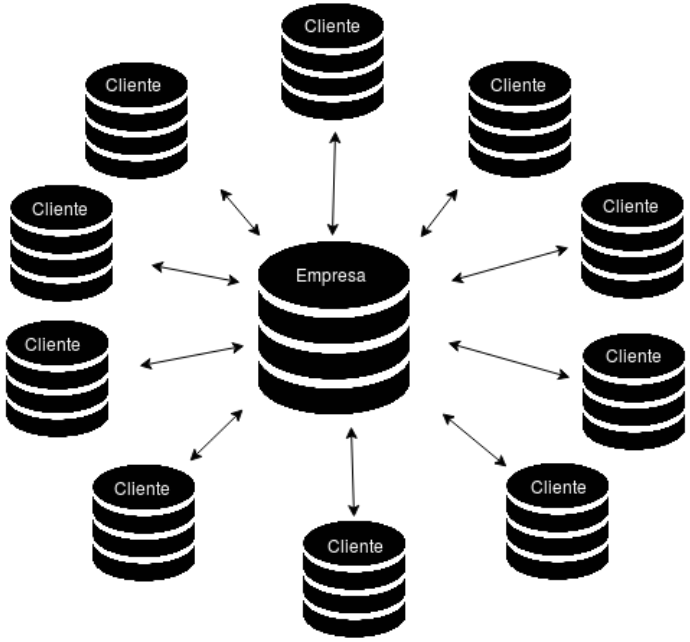
\includegraphics[width=0.6\textwidth]{Esquema_Rede} % Include the image placeholder.png
		\caption[Esquema de rede]{Esquema da rede criada com o sistema central na empresa promotora e os sistemas locais nos clientes}
		\label{fig:intro1}
	\end{center}
\end{figure}
Para consultar a informação nas bases de dados propõem-se uma aplicação em ambiente \textit{Web}, disponível em qualquer momento e dispositivo. A aplicação deve permitir que utilizadores sem conhecimentos sobre bases de dados comuniquem com estas de forma a consultar a informação desejada. Assim sendo enumeram-se os objetivos principais do projeto:
\begin{enumerate}
	\item Criar uma infraestrutura de bases de dados
	\item Criar uma aplicação \textit{Web} para consultar os históricos
\end{enumerate}
Como requerimento definiu-se que deve ser dada prioridade à utilização de \textit{software} gratuito. Além disto, dada a quantidade de opções disponíveis no mercado, definiu-se também que a solução desenvolvida deve ser simples de forma a promover a sua portabilidade para outras plataformas e linguagens.
\newpage
Este relatório está divido em capítulos, divididos da seguinte maneira:
\begin{itemize}
	\item \autoref{chap:intro} descreveu-se os objetivos do projeto e apresentou-se a solução proposta
	\item \autoref{chap:conceitos} consiste numa explicação de alguns conceitos necessários importantes para a criação de bases de dados relacionais e nas ferramentas utilizadas para desenvolver este projeto
	\item \autoref{chap:solucao} explica a infraestrutura de bases de dados proposta, desenvolvida para uma utilização a baixo nível
	\item \autoref{chap:aplicacao} descreve algumas adições à infraestrutura proposta e as funcionalidades da aplicação de gestão do sistema
	\item \autoref{chap:usabilidade} apresenta resultados de testes realizados com utilizadores à aplicação de gestão do sistema
	\item \autoref{chap:conclusoes} contém comentários sobre a solução desenvolvida e ideias para trabalhos futuros que a possam complementar
\end{itemize}

\cleardoublepage
\chapter{Conceitos e Ferramentas de Desenvolvimento}
\label{chap:conceitos}
\section{Moldes de injeção}
\begin{figure}[H]
	\begin{center}
		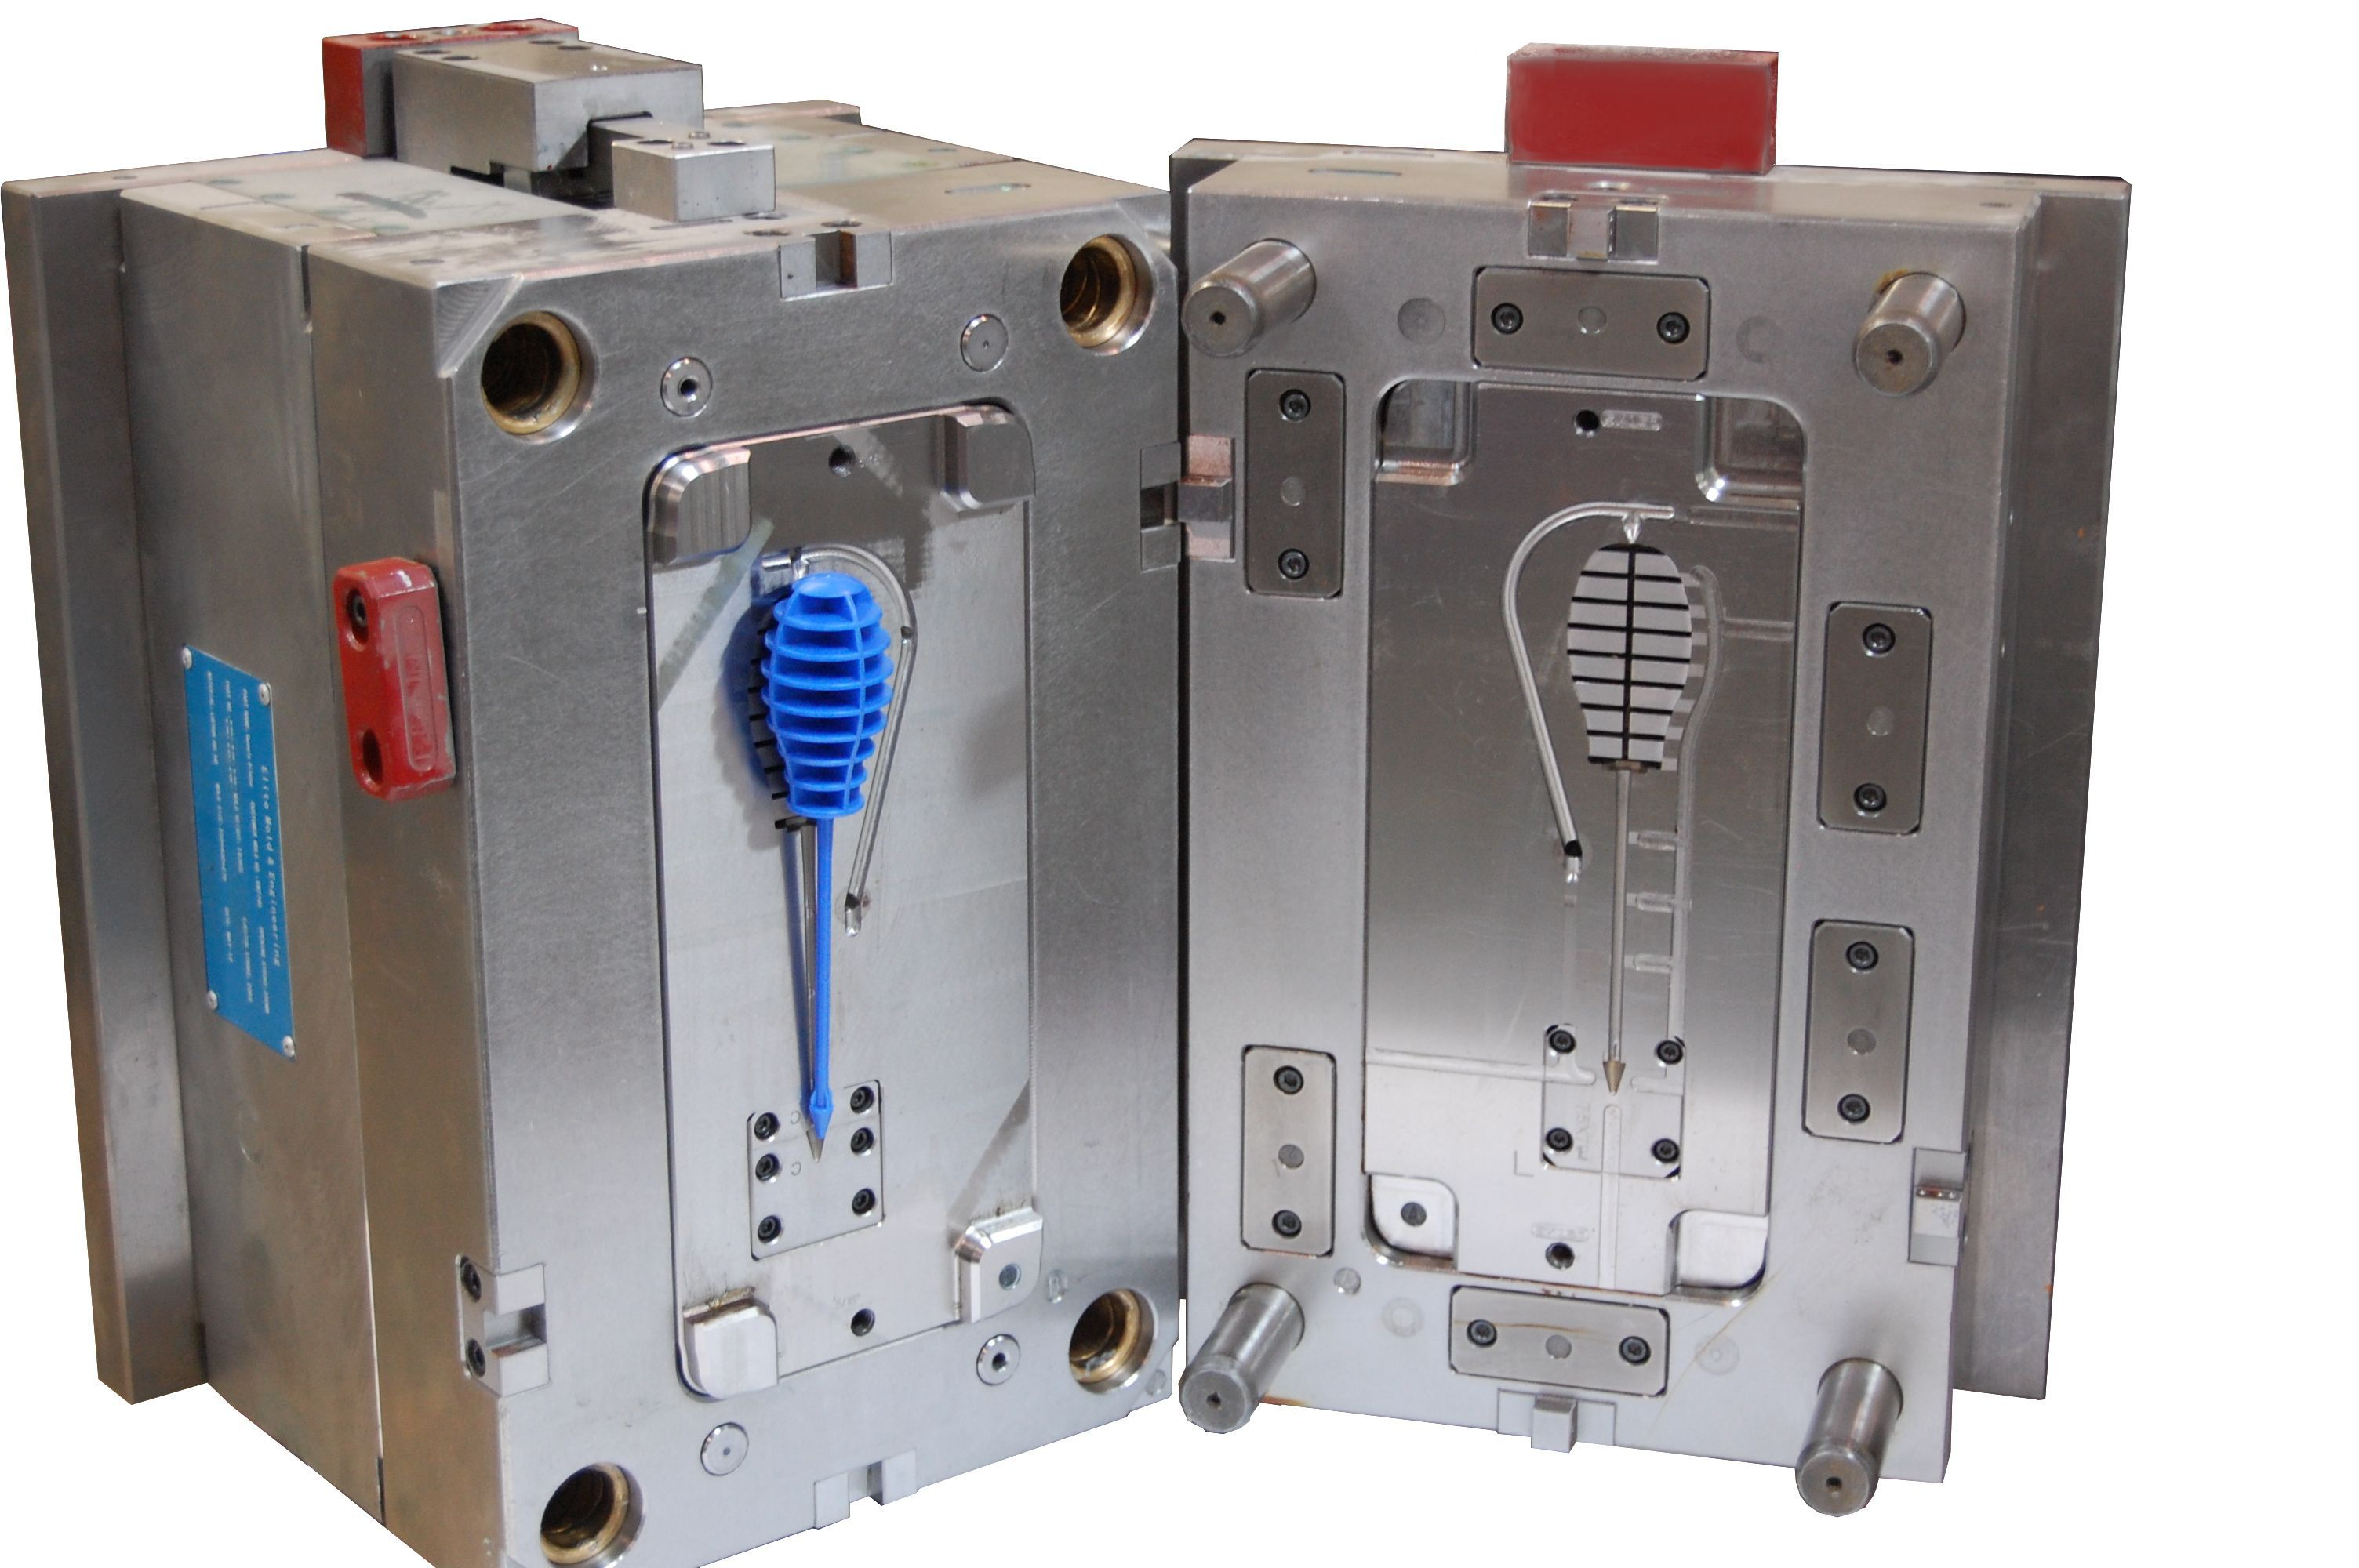
\includegraphics[width=0.75\textwidth]{molde} % Include the image placeholder.png
		\caption[Molde de injeção]{Molde de injeção aberto com a peça realizada \cite{molde_imagem}}
		\label{fig:molde}
	\end{center}
\end{figure}
Moldagem é o processo mecânico de dar forma a um material no estado líquido usando um molde \cite{definicao_moldagem,definicao_moldar}. Um molde é uma ferramenta sólida oca desenvolvida para efeitos de fundição \cite{definicao_molde}. Esta é enchida com um material em estado liquido ou em pó como plástico, metal, cerâmica ou vidro \cite{Williams1975,Trovant1998,JanneyMarkA.Knoxville1991,Yan2009}.\par
A moldagem por injeção é particularmente útil na produção em massa de peças de plástico com elevada complexidade geométrica \cite{Shen,Shelesh}. Estas podem ser encontradas em todas as áreas da industria como por exemplo empacotamento, aviação, construção e eletrónica \cite{Ozcelik}. Neste processo, plástico quente é forçado para dentro de um molde frio com a forma desejada. O material cobre todas as feições do molde e vai endurecendo sobre o efeito de altas pressões. O processo de injeção pode ser divido em fases distintas \cite{Shen}:
\begin{itemize}[noitemsep]
	\item Fecho do molde
	\item Enchimento
	\item Compactação
	\item Abertura do molde
	\item Extração
\end{itemize}
Em 1868, John Wesley Hyatt inventou uma maneira de fazer bolas de bilhar injetando celuloide para dentro de um molde \cite{historia,patente1868}.\par
Em 1872 Jonh e o seu irmão Isaiah patentearam a primeira máquina de moldes de injeção. Esta era relativamente simples comparada às que são usadas hoje em dia na indústria. Consistia de um pequeno embolo para injetar plástico num molde através de um cilindro quente \cite{historia,patente1872}.\par
A indústria cresceu lentamente produzindo artigos de plástico como botões e pentes. Nos anos 40 a utilização de moldes de injeção cresceu por causa da Segunda Guerra Mundial que tinha uma grande procura de produtos baratos e produzidos em massa \cite{historia}.\par
Em 1946, James Hendry construiu a primeira máquina de moldes de injeção com um sem fim, revolucionando a indústria dos plásticos com um design para substituir o embolo de Hyatt. Este sem fim é colocado dentro do cilindro e mistura o material a ser moldado antes de ser injetado no molde. Isto permitiu que cor ou plástico reciclado fossem adicionados à mistura \cite{historia,patente1946}.\par
A qualidade de fabrico dos moldes e das peças produzidas evoluiu com o passar do tempo. A industria investiu em técnicas sofisticadas no desenvolvimento de moldes, para que estes não contenham falhas, e no uso de materiais com qualidade elevada para evitar o desgaste da ferramenta. No entanto, dificilmente se atinge peças com a qualidade desejada unicamente através das ferramentas desenvolvidas. É necessário implementar também técnicas de monitorização de qualidade \cite{Woll}.


\section{Base de dados relacional}
Bases de dados e sistemas de gestão de bases de dados são uma componente essencial na vida da sociedade moderna: muitos de nós realizamos ações todos os dias que envolvem interações com bases de dados. Por exemplo, o ato de depositar e levantar dinheiro num banco, reservar estadias e voos ou comprar alguma coisa online podem envolver alguém ou um algum programa informático que acede a uma base de dados \cite{Elmasri:2010:FDS:1855347}.\par
Esta tecnologia tem um impacto cada vez maior no uso dos computadores. É seguro afirmar que as bases de dados desempenham um papel crítico em quase todas as áreas onde são usados computadores \cite{Elmasri:2010:FDS:1855347}.\par
Uma base de dados é uma coleção organizada de dados que estão relacionados e que podem ser partilhados por múltiplas aplicações \cite{definicao_base_dados}. São considerados dados factos reais que podem ser registados e têm um significado implícito, como por exemplo, nomes, moradas e números de telefone. Uma base de dados tem uma fonte de onde os dados são provenientes, algum grau de interação com eventos do mundo real e uma audiência que está ativamente interessada no seu conteúdo \cite{Elmasri:2010:FDS:1855347}.\par
A implementação destas é garantida por parte de um sistema de gestão de base de dados. Este é um \textit{software} de que facilita os processos de definir, construir, manipular e partilhar bases de dados entre vários utilizadores e aplicações. Definir uma base de dados envolve especificar o tipo de dados, estruturas e restrições dos dados a serem armazenados. Construir é o processo de guardar dados e armazena-los num local definido pelo sistema de gestão de bases de dados. Manipular inclui funções como realizar \textit{queries} à base de dados e receber informação específica, altera-la de acordo com mudanças nas variáveis e gerar relatórios a partir dos dados presentes. Partilhar permite que múltiplos utilizadores e programas acedam à base de dados simultaneamente \cite{Elmasri:2010:FDS:1855347}.\par
Outras funções importantes fornecidas pelos sistemas de gestão de bases de dados incluem proteger e manter a base de dados durante um longo período de tempo. Proteger inclui proteção contra falhas de \textit{hardware} e \textit{software} e segurança contra acessos maliciosos ou não autorizados. Tipicamente uma grande base de dados pode ter um tempo de vida de vários anos, então o sistema de gestão de bases de dados tem de fornecer ferramentas para manter a base de dados de forma a permitir que o sistema evolua com novos requerimentos que surjam ao longo do tempo \cite{Elmasri:2010:FDS:1855347}.
Para completar estas definições iniciais, chama-mos sistema de base de dados ao conjunto das bases de dados com o sistema de gestão de bases de dados como representado na \autoref{fig:relacional1}.
\begin{figure}[H]
	\begin{center}
		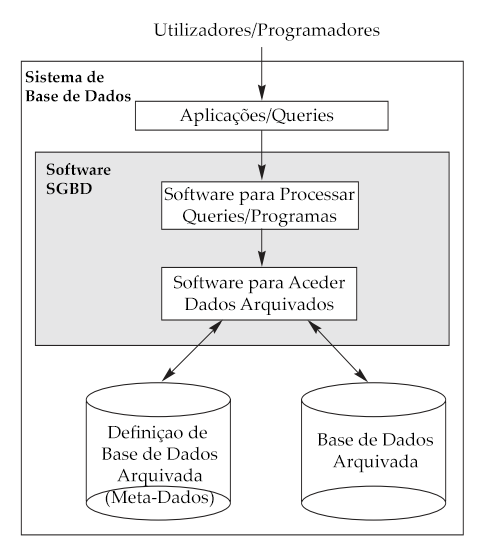
\includegraphics[width=0.7\textwidth]{SGBD} % Include the image placeholder.png
		\caption[Esquema de um sistema de bases de dados]{Esquema simplificado de um sistema de bases de dados \cite{Elmasri:2010:FDS:1855347}}
		\label{fig:relacional1}
	\end{center}
\end{figure}
O modelo relacional foi primeiramente introduzido por Ted Codd do \textit{IBM Research} em 1970 \cite{Elmasri:2010:FDS:1855347,Codd} e atraiu imediatamente atenção pela sua simplicidade e base matemática. O modelo utiliza o conceito matemático de $ " $relação$ " $ representado por tabelas e é baseado na teoria dos conjuntos \cite{Elmasri:2010:FDS:1855347}.\par
As primeiras implementações comerciais do modelo relacional ficaram disponíveis no inicio dos anos 80, como o \textit{SQL/DS} no sistema operativo \textit{MVS} do \textit{IBM} e o sistema de gestão de base de dados \textit{Oracle}. Desde aí, o modelo tem sido implementado num grande número de sistemas comerciais. Os sistemas de gestão de bases de dados relacionais populares atualmente incluem \textit{DB2} e \textit{Informix Dynamic Server} (do \textit{IBM}), \textit{Oracle} e \textit{Rdb} (da \textit{Oracle}), \textit{Sybase} (da \textit{Sybase}) e \textit{SQLServer} e \textit{Access} (da \textit{Microsoft}). Existem também vários sistemas grátis como \textit{MySQL} e \textit{PostgreSQL} \cite{Elmasri:2010:FDS:1855347}.\par
Modelos de dados que procederam o relacional incluem os modelos hierárquicos e de rede. Estes foram propostos nos anos 60 e foram implementados nos primeiros sistemas de gestão de bases de dados nos anos 60 e 70. Estes modelos tiveram bastante importância na história das bases de dados e são referidos atualmente como sistemas de bases de dados \textit{legacy} \cite{Elmasri:2010:FDS:1855347}.

\subsection{Domínios, Atributos, Tuplos e Relações}
Um domínio é um conjunto atómico de valores. Atómico significa que cada valor num dado domínio é único e indivisível. Um método comum de especificar um domínio é especificar o tipo de dados do mesmo. Além disto, também é útil dar nomes aos domínios. Por exemplo, a informação de números de telemóvel pode ser guardada num domínio onde o seu tipo de dados é um inteiro de nove dígitos \cite{Elmasri:2010:FDS:1855347}.\par
Um esquema de relação é constituído por um nome de uma relação e uma lista de atributos. Cada atributo é o nome do papel desempenhado por domínio no esquema da relação. É possível múltiplos atributos terem o mesmo domínio \cite{Elmasri:2010:FDS:1855347}.\par 
O esquema de relação é um grupo de múltiplos tuplos. Cada tuplo é um conjunto de valores ordenados que estão associados diretamente a um atributo \cite{Elmasri:2010:FDS:1855347}. A \autoref{fig:relacional2} representa um exemplo do que foi dito anteriormente.
\vspace{1cm}
\begin{figure}[H]
	\hspace{-2cm}
	
		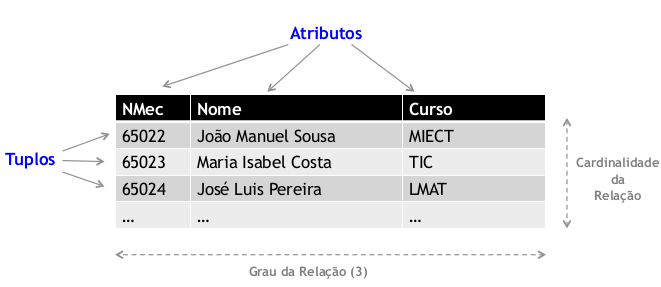
\includegraphics[width=0.9\textwidth]{exemplo_relacional} % Include the image placeholder.png
		\caption[Exemplo de atributos e tuplos]{Exemplo onde é possível observar a relação com os seus atributos e alguns tuplos}
		\label{fig:relacional2}
	
\end{figure}

\newpage
\subsection{Análise de requisitos}
A análise de requisitos é o primeiro passo necessário para definir uma base de dados. Este processo envolve uma comunicação com a entidade que deseja adquirir a base de dados e pode ser sumariza-do nos seguintes passos:
\begin{enumerate}
	\item Numa primeira fase realiza-se uma recolha detalhada de toda a informação referente ao problema do mundo real e retirar entidades, atributos, restrições, etc.
	\item Filtrar a informação de forma a remover redundâncias e informação pouco relevante
	\item Clarificar aspetos pouco claros
	\item Completar o problema com informação adicional necessária
	\item Distinguir dados de operações
\end{enumerate}
Este processo é transversal ao modelo de dados escolhido para realizar a base de dados. Para uma base de dados relacional é necessário identificar as chaves de uma relação:
\begin{itemize}
	\item Superchave - Conjunto de atributos que identificam de forma única dois tuplos distintos
	\item Chave candidata - são todas as superchaves que não podem ser mais simplificadas
	\item Chave primária - escolhida do conjunto de chaves candidatas e identifica de forma única o tuplo
	\item Chave única - restantes chaves candidatas que não foram escolhidas como chave primária
	\item Chave estrangeira - conjunto de atributos que é chave primária de outra relação
\end{itemize}
A escolha da chave primária pode ser feita de forma aleatória mas, priorizam-se chaves que identifiquem de forma natural um atributo. Por exemplo: uma pessoa pode ser identificada por um número de identificação, número de identificação fiscal ou pelo seu número de telefone dado que estes nunca se repetem. O número de identificação é mais natural para identificar uma pessoa do que o seu número de identificação fiscal e menos volátil do que o seu número de telefone, dado que este pode ser alterado.\par 
Para realizar um Diagrama Entidade Relação são necessárias informações sobre a relação entre as entidades, a cardinalidade e a obrigatoriedade de participação na relação. Estas são deduzidas durante a análise de requisitos mas serão explicadas na \autoref{subchap:DER}.

\subsection{Diagrama Entidade Relação}
\label{subchap:DER}
A representação lógica dos dados é uma componente importante na área das bases de dados. Existem vários modelos para esta representação antes da criação do modelo entidade-relação apresentado por P. P. Chen em 1976, sendo os mais conhecidos os modelos em rede, relacional e entidade. Estes modelos têm as suas vantagens e desvantagens. O modelo em rede permite uma vista mais natural dos dados dividindo-os em entidades e relações (até um determinado ponto), mas a sua capacidade de garantir independência dos dados foi superada. O modelo relacional consegue ter um grande grau de independência dos dados, mas pode perder alguma informação semântica importante sobre o mundo real. O modelo de entidade também consegue um grande grau de independência dos dados, mas a forma visualizar os dados não é tão fácil para algumas pessoas \cite{Chen}.\par
O modelo entidade-relação adota uma vista mais natural em que o mundo real consiste de entidades e relações, incorpora alguma informação semântica importante sobre o mundo real e consegue ter um grande grau de independência de dados. O modelo entidade-relação é baseado na teoria das relações e foi desenvolvido com o objetivo de servir de base para um sistema de visualização de dados unificado \cite{Chen}.\par
O diagrama entidade-relação é uma representação gráfica da análise de requisitos realizada anteriormente baseada no modelo entidade-relação. Este diagrama não é determinístico pois, para uma mesma análise, podem nascer diferentes diagramas que cumprem todos os requisitos.\par
Um diagrama é constituído elementos como entidades, atributos e relações. Uma entidade é algo que existe no mundo real como uma pessoa ou um carro. Um atributo é uma característica da entidade como uma pessoa tem um nome e um carro tem uma matricula. Uma relação é como uma ou mais entidades interagem entre si como uma pessoa tem um carro \cite{Chen}.\par 
Passando à notação, as entidades são representadas por caixas retangulares, os atributos por caixas ovais e as relações por caixas em forma de losango como mostra a \autoref{fig:der1}. Os atributos sublinhados representam a chave primária da entidade.
\begin{figure}[H]
	\begin{center}
		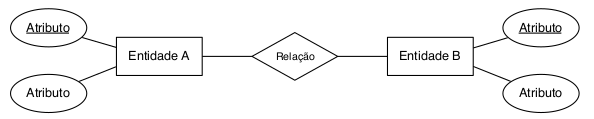
\includegraphics[width=0.8\textwidth]{notacao1} % Include the image placeholder.png
		\caption[Representação de entidades, relações e atributos]{Representação das entidades Pessoa e Carro, uma pessoa identificada pelo número de ID civil tem um carro identificado pela sua matrícula}
		\label{fig:der1}
	\end{center}
\end{figure}
As entidades podem ser fortes e fracas. Uma entidade forte não depende de outras entidades, enquanto uma entidade fraca necessita de ser identificada em conjunto com uma entidade forte. As relações de identificação definem a ou as entidades fortes que identificam uma entidade fraca entre as quais esta se relaciona. As entidades fracas são representadas por caixas retangulares com linha dupla e as relações de identificação são identificadas por um losango de linha dupla como representado na \autoref{fig:der2}.
\begin{figure}[H]
	\begin{center}
		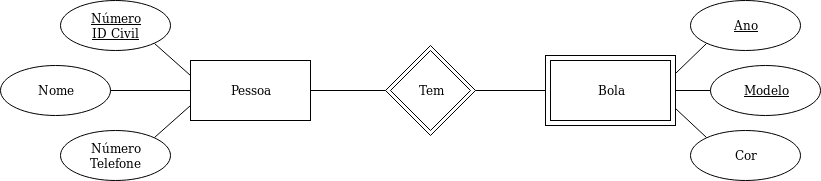
\includegraphics[width=0.8\textwidth]{notacao2} % Include the image placeholder.png
		\caption[Representação de entidades fortes e fracas e relação de identificação]{Representação das entidades Pessoa e Bola, uma pessoa identificada pelo número de ID civil tem uma bola de um determinado modelo e ano. A bola não tem um elemento caracterizador único pois podem existir bolas do mesmo modelo e ano, então identifica-se esta em conjunto com informação da pessoa que tem a bola}
		\label{fig:der2}
	\end{center}
\end{figure}
\newpage
Para completar a relação entre entidades é necessário identificar também o grau, cardinalidade e obrigatoriedade de participação de uma relação. Quanto ao grau, uma relação pode ser unária, binária ou ternária como representado na \autoref{fig:der3}. As relações ternárias podem ser decompostas em relações binárias, como mostra a \autoref{fig:der4}.
\vspace{2cm}
\begin{figure}[H]
	\centering
	\begin{minipage}{0.5\textwidth}
		\vspace{-1cm}
		\begin{center}
			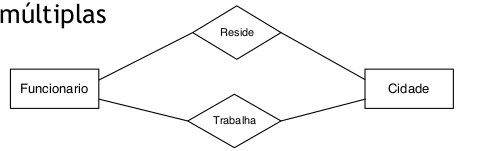
\includegraphics[width=.25\textwidth]{notacao3} % Include the image placeholder.png
			\subcaption{Exemplo de relação unária onde uma\\pessoa casa com outra pessoa}
			\label{fig:der31}
		\end{center}
	\end{minipage}%
	\begin{minipage}{0.5\textwidth}
		\begin{center}
			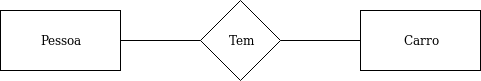
\includegraphics[width=0.9\textwidth]{notacao4} % Include the image placeholder.png
			\subcaption{Exemplo de relação binária onde uma pessoa tem um carro}
			\label{fig:der32}
		\end{center}
	\end{minipage}
	\begin{minipage}{0.5\textwidth}
		\vspace{1cm}
		\begin{center}
			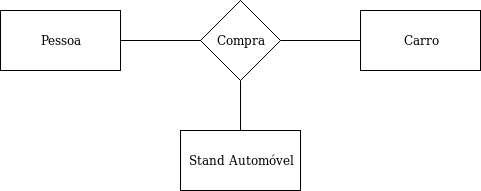
\includegraphics[width=0.9\textwidth]{notacao5} % Include the image placeholder.png
			\subcaption{Exemplo de relação ternária onde uma pessoa compra um carro a um stand automóvel}
			\label{fig:der33}
		\end{center}
	\end{minipage}
	\caption{Representação dos graus de relações}
	\label{fig:der3}
\end{figure}
\vspace{1cm}
\begin{figure}[H]
	\begin{center}
		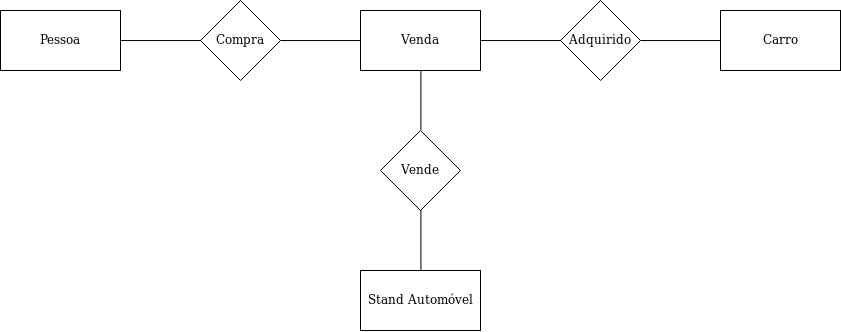
\includegraphics[width=.75\textwidth]{notacao6} % Include the image placeholder.png
		\caption[Exemplo de decomposição de uma relação ternária em relações binárias]{Exemplo de decomposição da relação ternária da \autoref{fig:der33} em relações binárias. A entidade venda relaciona de forma mais simples a pessoa, o carro e o stand automóvel envolvidos na compra}
		\label{fig:der4}
	\end{center}
\end{figure}

\newpage
As relações podem também ser múltiplas, ou seja, mais do que uma relação entre entidades como demonstrado na \autoref{fig:der8}.
\begin{figure}[H]
	\begin{center}
		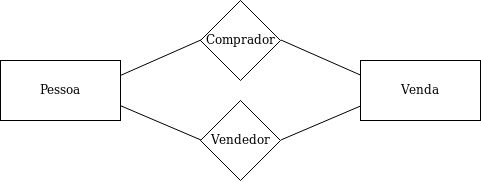
\includegraphics[width=0.5\textwidth]{notacao7} % Include the image placeholder.png
		\caption[Representação de múltiplas relações entre duas entidades]{Representação de múltiplas relações entre duas entidades, no ato de venda uma pessoa é o vendedor e outra é o comprador}
		\label{fig:der8}
	\end{center}
\end{figure}
Quanto à cardinalidade uma relação pode ser de três tipos:
\begin{itemize}[noitemsep]
	\item 1 para 1
	\item 1 para N ou N para 1
	\item N para M
\end{itemize}
A \autoref{fig:der5} apresenta uma representação visual destas cardinalidades e a \autopageref{fig:der6} apresenta a notação da cardinalidade definida por Chen.
\begin{figure}[H]
	\centering
	\begin{minipage}{0.3\textwidth}
		\vspace{-.5cm}
		\begin{center}
			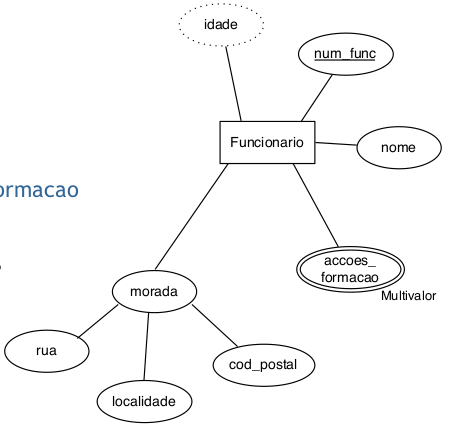
\includegraphics[width=0.4\textwidth]{notacao8} % Include the image placeholder.png
			\subcaption{Relação 1 para 1}
			\label{fig:der51}
		\end{center}
	\end{minipage}%
	\begin{minipage}{0.3\textwidth}
		\begin{center}
			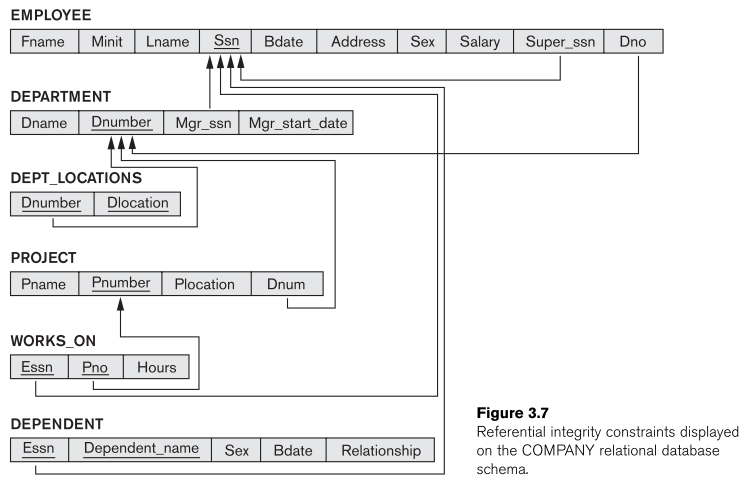
\includegraphics[width=0.4\textwidth]{notacao9} % Include the image placeholder.png
			\subcaption{Relação 1 para N\\ou N para 1}
			\label{fig:der52}
		\end{center}
	\end{minipage}%
	\begin{minipage}{0.3\textwidth}
		\begin{center}
			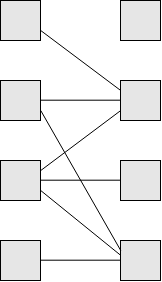
\includegraphics[width=0.4\textwidth]{notacao10} % Include the image placeholder.png
			\subcaption{Relação N para M\\ou muitos para muitos}
			\label{fig:der53}
		\end{center}
	\end{minipage}
	\caption{Representação dos tipos de cardinalidade}
	\label{fig:der5}
\end{figure}
\vspace{.5cm}
\begin{figure}[H]
	\centering
	\begin{minipage}{1\textwidth}
		\begin{center}
			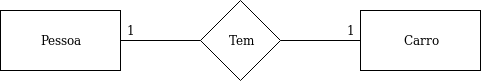
\includegraphics[width=.5\textwidth]{notacao11} % Include the image placeholder.png
			\subcaption{1 pessoa pode ter 1 carro}
			\label{fig:der61}
		\end{center}
	\end{minipage}
	\begin{minipage}{1\textwidth}
		\begin{center}
			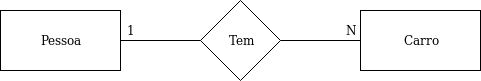
\includegraphics[width=0.5\textwidth]{notacao12} % Include the image placeholder.png
			\subcaption{1 pessoa pode ter N carros}
			\label{fig:der62}
		\end{center}
	\end{minipage}
	\caption{Notação da cardinalidade de Chen}
	\label{fig:der6}
\end{figure}
A obrigatoriedade de participação numa relação define se uma entidade tem de participar obrigatoriamente na relação. Esta é representada por uma linha dupla na ligação com a relação como representado na Figura \ref{fig:der9}. 
\begin{figure}[H]
	\begin{center}
		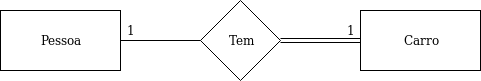
\includegraphics[width=0.5\textwidth]{notacao13} % Include the image placeholder.png
		\caption[Representação da obrigatoriedade de participação]{Representação da obrigatoriedade de participação. Neste caso uma pessoa pode ter ou não carro mas, um carro tem de pertencer sempre a uma pessoa}
		\label{fig:der9}
	\end{center}
\end{figure}
Os atributos também podem ser de tipos diferentes. Estes podem ser derivados, compostos ou multi-valor como mostra a \autoref{fig:der11}
\begin{figure}[H]
	\begin{center}
		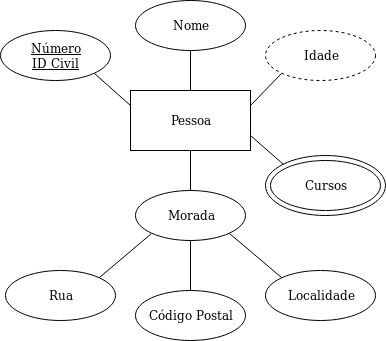
\includegraphics[width=0.5\textwidth]{notacao14} % Include the image placeholder.png
		\caption[Representação dos tipos de atributos]{Representação dos tipos de atributos. Os atributos derivados são representados a tracejado, os compostos têm sub-atributos associados a si e os multi-valor são representados com linha dupla. A idade varia com a data, uma pessoa pode ter um ou mais cursos e a morada pode ser dividida em rua, código postal e localidade}
		\label{fig:der11}
	\end{center}
\end{figure}

\subsection{Esquema Relacional}
O esquema relacional incluí todas as relações que concretizam uma base de dados. Cada relação é representada pelos seus atributos, tendo os atributos chave sublinhados. Quando atributos de relações diferentes representam o mesmo elemento do mundo real, estes são conectados. Quando um elemento aparece em relações diferentes significa que numa destas, o elemento, é atributo chave da relação e assim sendo, os restantes atributos são considerados chaves estrangeiras. São representados com a ligação ao atributo que serve de chave primária como demonstrado na \autoref{fig:er1} \cite{Chen}.
\begin{figure}
	\begin{center}
		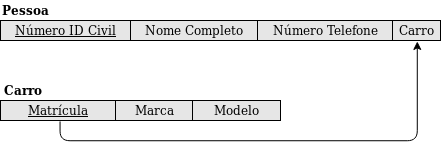
\includegraphics[width=0.7\textwidth]{notacao15} % Include the image placeholder.png
		\caption[Representação esquema relacional]{Representação do esquema relacional com as ligações das chaves estrangeiras deduzido do diagrama entidade relação da \autoref{fig:der61}}
		\label{fig:er1}
	\end{center}
\end{figure}
Este esquema pode ser deduzido a partir do diagrama entidade relação onde as entidades se traduzem em relações e as relações do diagrama representam as chaves estrangeiras no esquema relacional.

\section{\textit{Structured Query Language}}
A linguagem \textit{SQL} é considerada uma das maiores razões para o sucesso comercial das bases de dados relacionais. Porque se tornou normal a sua utilização em bases de dados relacionais, os utilizadores tiveram menos preocupações a transferir as suas aplicações de outros tipos de bases de dados - por exemplo, bases de dados hierárquicas e em rede - para uma base de dados relacional. Isto porque se um sistema de gestão de bases de dados não cumprisse os requisitos definidos, não era problemático transferir a solução para outro sistema de gestão de bases de dados dado que ambos utilizam a mesma linguagem. Na realidade existem várias sub-versões desta linguagem dependentes de cada sistema de gestão de bases de dados. No entanto, se o utilizador se limitar apenas às funções standard desta linguagem a mudança de sistema é bastante simplificada. Outra vantagem de ter uma linguagem normalizada é que uma aplicação pode utilizar informação de bases de dados em sistemas de gestão de bases de dados diferentes ao mesmo tempo \cite{Elmasri:2010:FDS:1855347}.\par 
O nome \textit{SQL} atualmente significa \textit{Structured Query Language}. Originalmente era chamado \textit{SQUEL} de \textit{Structured English QUEry Language}, foi desenhado e implementado no \textit{IBM Research} como uma interface experimental para o sistema de bases de dados relacionais \textit{SYSTEM R. SQL}. Um esforço conjunto entre o \textit{American National Standards Institute} (\textit{ANSI}) e a \textit{International Standards Organization} (\textit{ISO}) conduziu à normalização da versão do \textit{SQL} chamado SQL-86 ou SQL1. Surgiu depois uma versão expandida chamada SQL-92 ou SQL2. A seguinte versão reconhecida é o SQL:1999 ou SQL3. Dois \textit{updates} de depois resultaram nas versões SQL:2003 e SQL:2006  \cite{Elmasri:2010:FDS:1855347}. Sendo a atualização mais recente em 2016.\par 
O \textit{SQL} é uma linguagem básica para realizar \textit{queries} que permitem definir e construir uma base de dados, bem como interagir com os dados presentes nas bases de dados \cite{Elmasri:2010:FDS:1855347}.
%O \textit{SQL} é uma linguagem básica para realizar \textit{queries} dividida em dois campos principais, \textit{DDL} e \textit{DML}. \textit{DDL} ou \textit{Data Definition Language} são as \textit{queries} que permitem definir e construir uma base de dados. \textit{DML} ou \textit{Data Manipulation Language} são as \textit{queries} que permitem interagir com os dados\cite{Elmasri:2010:FDS:1855347}. Estas serão mais exploradas na \autoref{subchap:mysql}.

%\section{Tecnologias existentes}

\newpage
\section{\textit{Software} utilizado}
Para desenvolver as redes de bases de dados e aplicação escolheram-se os \textit{softwares} apresentados na \autoref{fig:softwares}. Como a solução será futuramente implementada em ambiente empresarial, definiu-se que não se deve usar \textit{softwares} que estejam em versão \textit{beta}. Além disto definiu-se que estes devem ser gratuitos.
\begin{figure}[H]
	\centering
	\begin{minipage}{0.33\textwidth}
		\vspace{0.88cm}
		\begin{center}
			
\includegraphics[width=0.3\textwidth]{ubuntu} % Include the image placeholder.png
			\subcaption{\textit{Ubuntu} \cite{ubuntu_logo}}
			\label{fig:linux}
		\end{center}
	\end{minipage}%
	\begin{minipage}{0.33\textwidth}
		\begin{center}
			
\includegraphics[width=0.4\textwidth]{gcc} % Include the image placeholder.png
			\subcaption{\textit{GNU} \cite{gcc_logo}}
			\label{fig:gcc}
		\end{center}
	\end{minipage}%
	\begin{minipage}{0.33\textwidth}
		\vspace{1.1cm}
		\begin{center}
			
\includegraphics[width=0.6\textwidth]{apache} % Include the image placeholder.png
			\subcaption{\textit{Apache} \cite{apache_logo}}
			\label{fig:apache}
		\end{center}
	\end{minipage}
	\begin{minipage}{1\textwidth}
		\vspace{0.5cm}
		\begin{center}
			
\includegraphics[width=0.25\textwidth]{mysql} % Include the image placeholder.png
			\subcaption{\textit{MySQL} \cite{mysql_logo}}
			\label{fig:mysql}
		\end{center}
	\end{minipage}
	\caption{Logótipos dos \textit{softwares} utilizados}
	\label{fig:softwares}
\end{figure}

\subsection{Ferramentas auxiliares}
Escolheu-se o \textit{Ubuntu} 16.04LTS como sistema operativo para os sistemas usados neste projeto, representado na \autoref{fig:linux}. Este é uma distribuição do \textit{Linux} baseado no \textit{Debian}. É um sistema operativo grátis e \textit{open source} desenvolvido pela \textit{Canonical}. A liberdade deste sistema operativo na área da programação criou uma comunidade de utilizadores que ajudam a pesquisar e desenvolver este sistema operativo \cite{ubuntu}.\par 
A \textit{Canonical} encarrega-se de garantir \textit{updates} de segurança e performance de forma regular. Apesar de não ser infalível o \textit{Linux} é um dos sistemas mais estáveis e menos provável de ser afetado por vírus, dado que a maior parte destes são desenhados para afetar sistemas operativos mais populares como o \textit{Windows} \cite{ubuntu}.\par
Escolheu-se utilizar \textit{C} no desenvolvimento deste projeto devido à afinidade com esta linguagem e com o facto do \textit{MySQL} disponibilizar protocolos oficiais e documentação de comunicação com esta linguagem \cite{mysql}.\par
O \textit{C} é uma linguagem para todos os tipos de problemas e importante no mundo da programação. Originalmente desenvolvido por Dennis Ritchie entre 1969 e 1973 no \textit{Bell Labs} e usado para re-implementar o sistema operativo \textit{Unix}. Desde então esta tornou-se uma das linguagens de programação mais popular de sempre com uma oferta de vários compiladores existentes no mercado. O \textit{C} foi então normalizado pelo \textit{ANSI} em 1989 e consequentemente pelo \textit{ISO}.\par 
No projeto usa-se o \textit{GNU Compiler Collection} (\textit{GCC}), representado na \autoref{fig:gcc}, como compilador dos programas em \textit{C}. Este foi desenvolvido primeiramente para o sistema operativo \textit{GNU} e focou-se em ser gratuito e garantir liberdade de programação ao utilizador. Conta com uma comunidade ativa que desenvolvem constantemente novas soluções e \textit{updates} regulares ao compilador de forma a que este não fique desatualizado \cite{gcc}.\par 
Escolheu-se utilizar \textit{Apache HTTP Server}, representado na \autoref{fig:apache} como servidor \textit{HTTP} para a aplicação \textit{Web}. Este foca-se em ser um servidor gratuito e garantir uma solução segura, eficiente e extensível \cite{apache}.\par
Lançado em 1995, tornou-se no \textit{software} mais utilizado pelas empresas para correr os seus \textit{sites}. Atualmente na versão 2.4, realizam \textit{updates} constantes ao programa para o manter estável e atualizado \cite{apache}.

\subsection{\textit{HTML}, \textit{JS} e \textit{PHP}}
\begin{figure}[H]
	\begin{center}
		
\includegraphics[trim={0 2.85cm 0 0},clip,width=0.4\textwidth]{web} % Include the image placeholder.png
		\caption[Representaçoã da ferramenta mais usada para desenvolver aplicações \textit{Web}]{Representação da ferramenta mais usada para desenvolver aplicações em ambiente \textit{Web} \cite{web_logo}}
		\label{fig:web}
	\end{center}
\end{figure}
Escolheu-se \textit{HTML}, \textit{JS} e \textit{PHP} para desenvolver a aplicação \textit{Web} deste projeto. Junto com \textit{SQL} e \textit{CSS} formam o conjunto de ferramentas mais usadas no desenvolvimento de aplicações \textit{Web} no mercado, representado na \autoref{fig:web}.\par 
\textit{HTML} ou \textit{Hyper Text Markup Language} descreve a estrutura da página \textit{Web} desenvolvida. Possuí elementos que funcionam como blocos para as páginas permitindo a criação de uma interface com um utilizador. \textit{CSS} ou \textit{Cascading Style Sheets} descreve como os elementos HTML devem ser dispostos na página, permitindo o desenvolvimento de uma interface mais apelativa. \textit{JS} ou \textit{JavaScript} permite interagir e alterar o código \textit{HTML} e \textit{CSS} criando uma interface mais interativa. Permite também desenvolver códigos e funções que são executadas no browser do cliente. \textit{PHP} ou \textit{PHP:Hypertext Preprocessor} permite desenvolver funções para aplicação que executam do lado do servidor. \textit{JS} e \textit{PHP} realizam ambos funções diferindo apenas no local onde são executadas \cite{web}. Sem contar com a interação com o \textit{HTML} e \textit{CSS}, o \textit{PHP} pode substituir o \textit{JS} como linguagem para criação de funções do sistema. No entanto, isto pode causar problemas de desempenho dado que o servidor terá de correr funções de todos os utilizadores. Assim sendo define-se que o uso do \textit{PHP} deve ser limitado a funções de sistema mais importantes, como conectar a uma base de dados em \textit{SQL}, e o \textit{JS} deve ser usado no desenvolvimento de funções de aplicação mais triviais.

\subsection{\textit{MySQL}}
\label{subchap:mysql}
Escolheu-se o \textit{MySQL}, representado na \autoref{fig:mysql}, como sistema de gestão de bases de dados relacionais para construir e utilizar as bases de dados usadas neste projeto, dada a sua simplicidade e velocidade de resposta. Existem outras ofertas gratuitas como o \textit{SQLite} e o \textit{PostgreSQL}. O \textit{SQLite} funciona apenas localmente e não permite uma conexão remota que se procura como solução para o problema. O \textit{PostgreSQL} é um sistema robusto que permite realizar tarefas que o \textit{MySQL} não consegue realizar. No entanto, dada a simplicidade da base de dados prevista na fase de projeto, não é necessário usar uma ferramenta tão completa e robusta \cite{mysqlvs}.\par 
O \textit{MySQL} é o mais popular e o sistema de gestão de bases de dados relacionais e o mais usado \cite{mysqlvs}. Garante um acesso múltiplo, rápido e robusto a uma base de dados no servidor. Foi desenvolvido para lidar com grandes quantidades de informação e \textit{softwares} com utilização massiva \cite{mysql}.\par 
O \textit{MySQL} oferece soluções gratuitas e pagas, \textit{Community} e \textit{Enterprise}, respetivamente. A primeira recebe menos \textit{updates} e correções que a solução paga. Tem também algumas funcionalidades bloqueadas e um limite na capacidade de sensivelmente 4Gb \cite{mysql}. Estas limitações não afetam o projeto e como tal opta-se pela solução gratuita deste \textit{software}.\par
Como referido anteriormente os vários sistemas de gestão de bases de dados possuem as suas próprias sub-versões da linguagem \textit{SQL} e, o \textit{MySQL}, não é exceção. Segue-se a lista com os comandos principais utilizados neste projeto \cite{mysql}:
\begin{itemize}
	\item \textbf{SHOW DATABASES/TABLES} - mostra todas as bases de dados ou tabelas da base de dados (\textit{MySQL})
	\item \textbf{CREATE DATABASE/TABLE} - criar bases de dados ou tabelas
	\item \textbf{DROP DATABASE/TABLE} - eliminar bases de dados ou tabelas
	\item \textbf{SELECT FROM} - visualizar tuplos de uma tabela
	\item \textbf{INSERT} - inserir tuplos numa tabela
	\begin{itemize}
		\item \textbf{INTO} - se forem inseridos múltiplos tuplos e um não respeitar as restrições de integridade definidas, nenhum tuplo é inserido
		\item \textbf{IGNORE} - se forem inseridos múltiplos tuplos e um não respeitar as restrições de integridade, esse é descartado e os restantes são inseridos na tabela (\textit{MySQL})
	\end{itemize}
	\item \textbf{DELETE} - elimina tuplos de uma tabela
	\item \textbf{UPDATE} - altera tuplos de uma tabela
	\item \textbf{GRANT} - dar privilégios a um utilizador
\end{itemize}
A \textit{querie} do tipo SELECT permite adicionar condições do tipo \cite{mysql}:
\begin{itemize}
	\item \textbf{WHERE} - definir parâmetros de busca de um atributo
	\item \textbf{GROUP BY} - permite agrupar informação permitindo operações matemáticas sobre valores, por exemplo: contagem, soma, média, etc.
	\item \textbf{ORDER BY} - escolher a ordem dos tuplos
\end{itemize}
As \textit{queries} do tipo DELETE e UPDATE  também permitem utilizar a condição WHERE.\par 
Na criação das tabelas atribuem-se o nome dos atributos e o seu respetivo domínio. O \textit{MySQL} oferece vários tipos de dados, dos quais foram usados \cite{mysql}:
\begin{itemize}
	\item \textbf{VARCHAR(n)} - \textit{string} com tamanho máximo n
	\item \textbf{INT} - inteiro entre -2147483648 e +2147483647
	\item \textbf{TINYINT} - inteiro entre -128 e +127
	\item \textbf{FLOAT} - numérico com casa decimais
	\item \textbf{DATETIME} - data e hora no formato AAAA-MM-DD HH:MM:SS
\end{itemize}
Define-se também as restrições de integridade \cite{mysql}:
\begin{itemize}
	\item \textbf{PRIMARY KEY} - define chave primária
	\item \textbf{UNIQUE} - define chave única
	\item \textbf{FOREIGN KEY REFERENCES} - define a chave estrangeira e o atributo de referência
\end{itemize}
Estas restrições ou \textbf{CONSTRAINTS} podem e devem ser atribuídas um nome de forma a identifica-las em mensagens de erro. Além disto é possível definir o comportamento de uma restrição de uma chave estrangeira quando o atributo de referencia é alterado (\textbf{ON UPDATE}) ou eliminado (\textbf{ON DELETE}) \cite{mysql}:
\begin{itemize}
	\item \textbf{NO ACTION} - não deixa realizar a ação
	\item \textbf{CASCADE} - todas as chaves estrangeiras dependentes do atributo de referencia são alteradas ou eliminadas de acordo com este
	\item \textbf{SET NULL} - altera o valor da chave estrangeira para NULL
	\item \textbf{SET DEFAULT} - altera o valor da chave estrangeira para um valor predefinido
\end{itemize}
O valor NULL representa um valor de um atributo que não existe ou é desconhecido, adiciona-se \textbf{NOT NULL} a um atributo quando este não pode assumir este valor \cite{mysql}.\par 
Estes são os comandos e conceitos principais que surgem ao longo deste documento. Como referido anteriormente e é possível observar aqui, o \textit{SQL} é uma linguagem simples e auto-explicativa.

\cleardoublepage
\chapter{Proposta de Solução}
\label{chap:solucao}
A infraestrutura de dados desenvolvida tem como objetivo ser simples, funcional a baixo nível e sem impor restrições na instrumentação dos moldes. Este capítulo descreve o processo de desenvolvimento das bases de dados, o método de transferência de medições, a gestão de \textit{backups}, as permissões dos utilizadores e um simples simulador de valores.

\section{Infraestrutura de Dados}
A instrumentação dos moldes geram valores localmente nos clientes e estes devem ser guardados numa base de dados central. A transferência é realizada usando protocolos TCP/IP. A fim de minimizar a perda de valores em caso de falha de conexão, coloca-se uma base de dados local em cada cliente, como representado na \autoref{fig:infra1}.
\begin{figure}[H]
	\begin{center}
		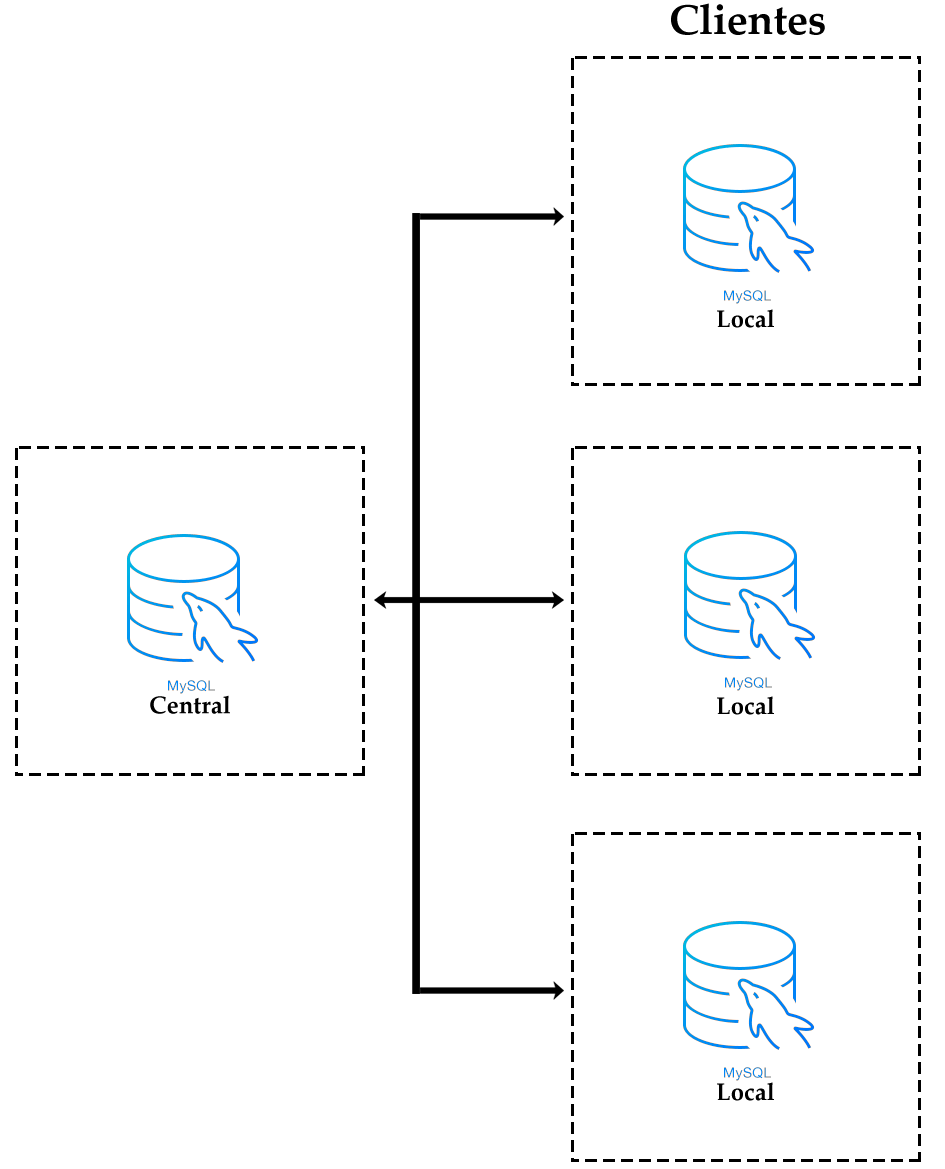
\includegraphics[width=0.44\textwidth]{Esquema_Projeto_4} % Include the image placeholder.png
		\caption[Diagrama das bases de dados]{Diagrama da infraestrutura com múltiplas bases de dados locais conectadas a uma base de dados central}
		\label{fig:infra1}
		\end{center}
\end{figure}
Para estabelecer o fluxo de informação desenvolveu-se um programa de transferência e um simulador, ambos desenvolvidos em \textit{C}. O programa de transferência envia \textit{queries} para as bases de dados locais e recebe respostas com valores que regista na base de dados central. O simulador gera valores para popular as bases de dados locais. Para simular múltiplos clientes usam-se simuladores independentes entre si, como representado na \autoref{fig:infra2}.
\begin{figure}[H]
	\begin{center}
		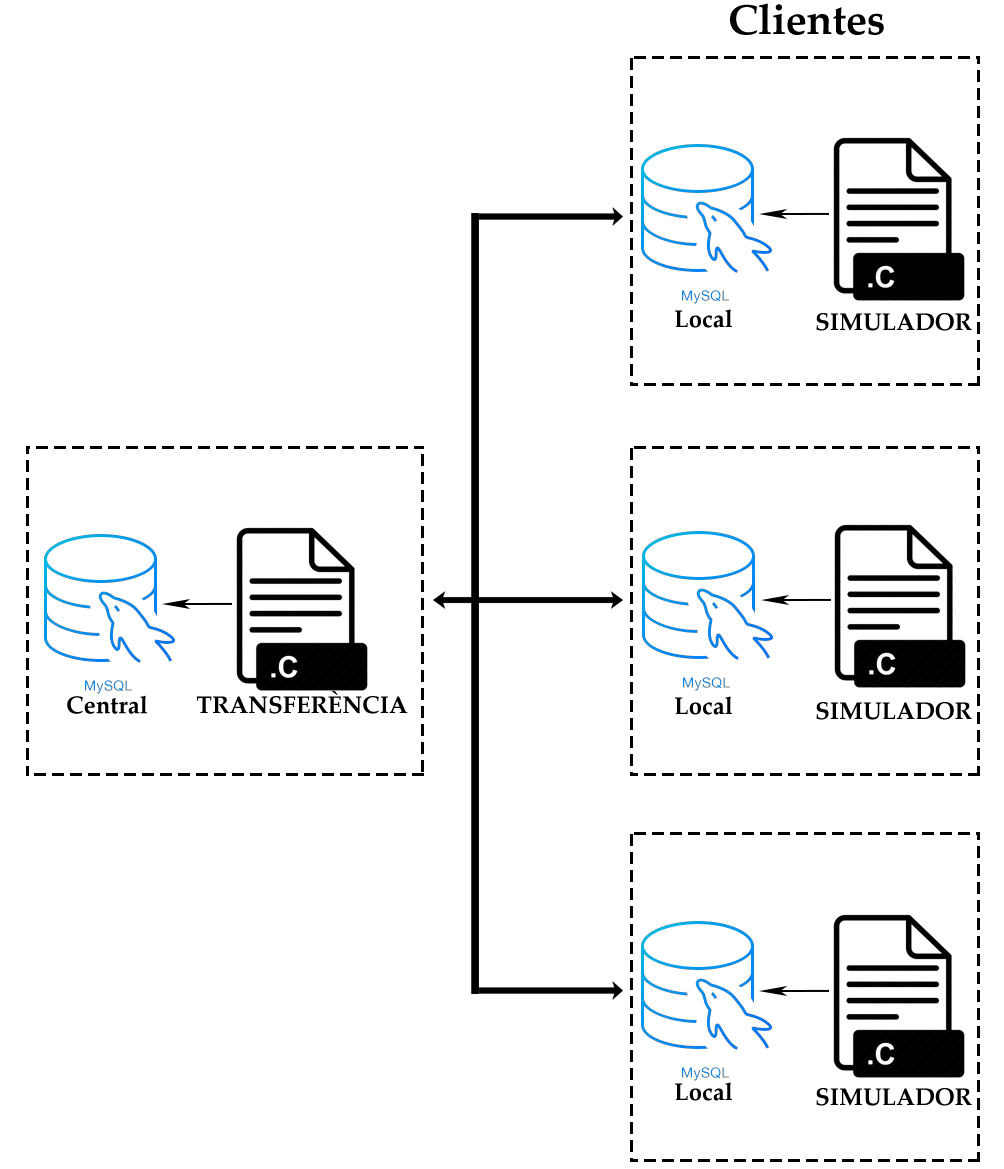
\includegraphics[width=0.55\textwidth]{Esquema_Projeto_5} % Include the image placeholder.png
		\caption[Diagrama do fluxo de informação]{Diagrama do fluxo de informação. Os simuladores substituem provisoriamente sistemas de aquisição de dados}
		\label{fig:infra2}
		\end{center}
\end{figure}
Para melhorar o desempenho da base de dados central e prevenir falhas críticas do sistema, desenvolveu-se um programa de gestão de \textit{backups}, também em \textit{C}. Este programa limpa e cria \textit{backups} da base de dados e guarda-os num repositório \textit{online}. De forma a não interferir diretamente com a informação da base de dados central criam-se duas bases de dados para a gestão dos \textit{backups}. Com esta adição, o esquema da infraestrutura final está representado na \autoref{fig:infra3}.\par 
\begin{figure}
	\begin{center}
		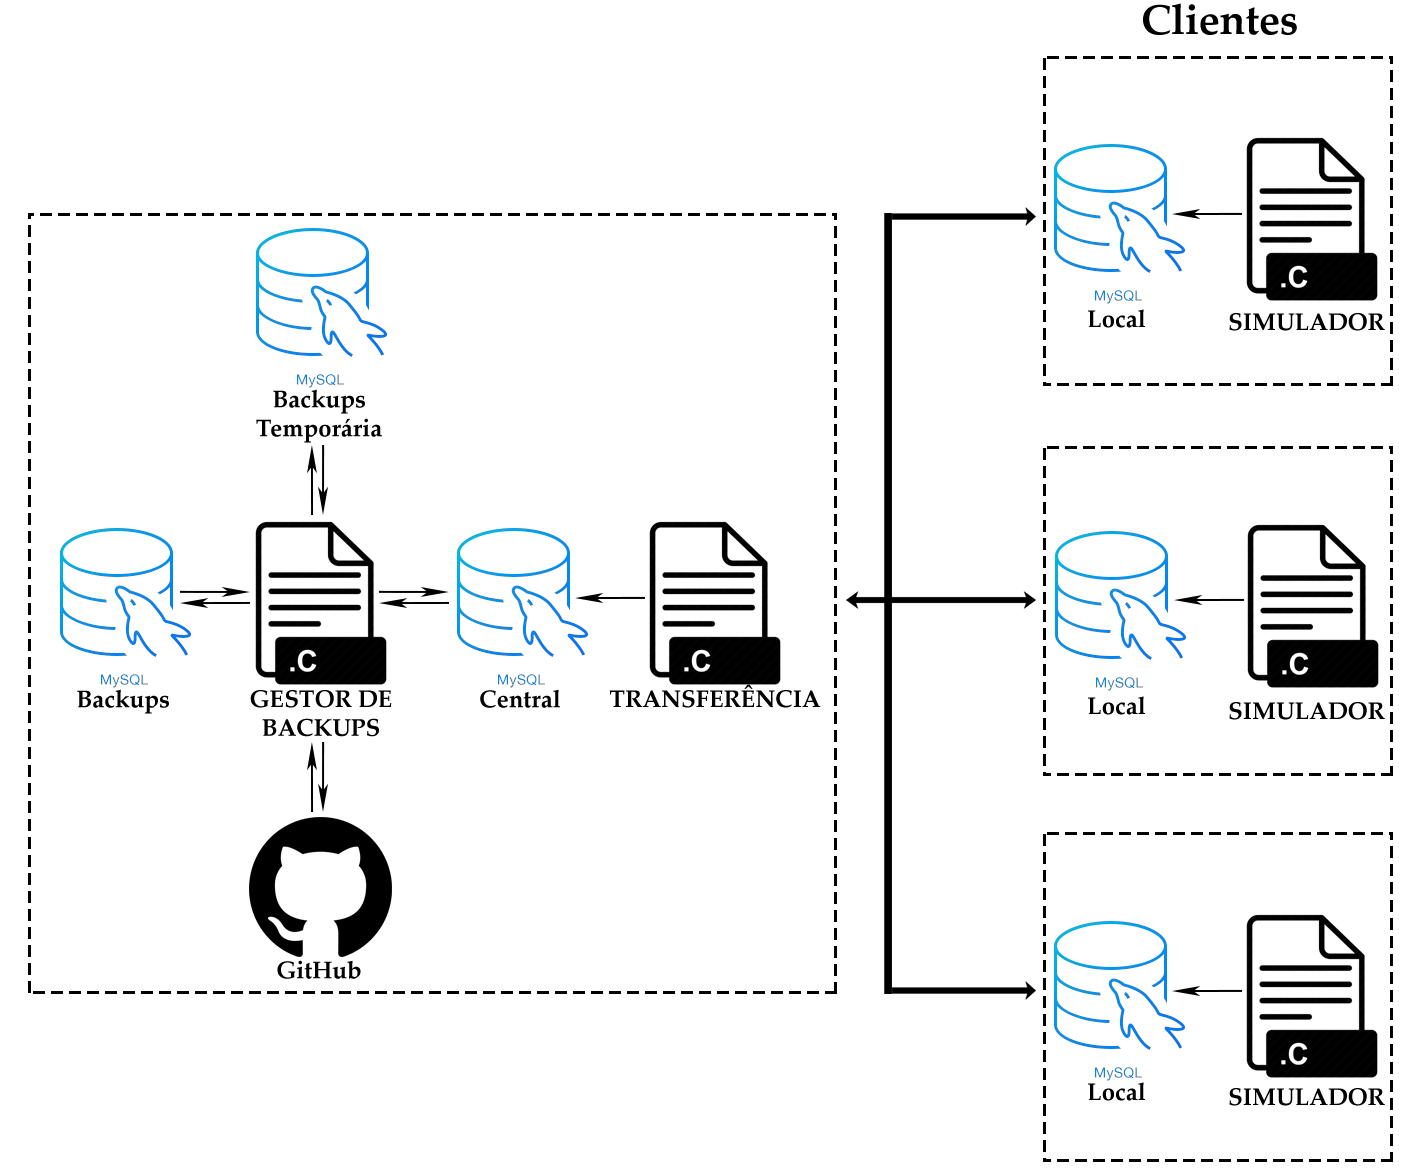
\includegraphics[width=1\textwidth]{Esquema_Projeto_6} % Include the image placeholder.png
		\caption[Diagrama final da infraestrutura]{Diagrama final da infraestrutura de dados. Os valores gerados nos simuladores são transferidos para a base de dados central. Estes valores são então processados pelo gestor de \textit{backups} que cria e guarda \textit{backups} provisoriamente num repositório online no \textit{GitHub}}
		\label{fig:infra3}
		\end{center}
\end{figure}

\section{Base de dados}
\subsection{Análise de requisitos}
Deseja-se, de uma forma geral, um sistema capaz de guardar remotamente medições realizadas em moldes instrumentados. Esta informação não é suficiente para se deduzir uma base de dados. Assim sendo, analisando e completando a informação inicial chega-se ao seguinte enunciado:\par 
%\vspace{2ex}
\textit{Um cliente, caracterizado por um ID, nome, morada, IP e port, tem moldes. Estes moldes são identificados por um ID, nome e descrição. Os moldes têm sensores com um número referente ao molde, tipo (termómetro, dinamómetro, extensómetro, etc.), nome e descrição. Estes sensores geram registos onde guardam a fase do processo (fecho do molde, enchimento, compactação, abertura e extração), data, hora, milissegundos e o valor num determinado momento.}\par 
\vspace{2ex}
Analisando este enunciado identificam-se as seguintes entidades com os seus respetivos atributos:
\begin{itemize}[noitemsep]
	\item Tipo
	\begin{itemize}[noitemsep]
		\item ID
		\item Nome
	\end{itemize}
	\item Fase
	\begin{itemize}[noitemsep]
		\item ID
		\item Nome
	\end{itemize}
	\item Clientes
	\begin{itemize}[noitemsep]
		\item ID de cliente único
		\item Nome
		\item Morada
		\item IP
		\item Port
	\end{itemize}
	\item Moldes
	\begin{itemize}[noitemsep]
		\item ID do cliente associado
		\item ID de molde único
		\item Nome
		\item Descrição
	\end{itemize}
	\item Sensores
	\begin{itemize}[noitemsep]
		\item ID do molde associado
		\item Número do sensor
		\item ID do tipo de sensor
		\item Nome
		\item Descrição
	\end{itemize}
	\item Registos
	\begin{itemize}[noitemsep]
		\item ID do molde associado
		\item Número do sensor associado
		\item ID da fase do processo
		\item Data
		\item Hora
		\item Milissegundos
		\item Valor
	\end{itemize}
\end{itemize}
\newpage
Analisando os atributos identificam-se as seguintes chaves primárias, únicas e estrangeiras:
\begin{itemize}[noitemsep]
	\item Tipo
	\begin{itemize}[noitemsep]
		\item Chave primária: ID
		\item Chaves únicas:
		\begin{enumerate}
			\item Nome
		\end{enumerate}
	\end{itemize}
	\item Fase
	\begin{itemize}[noitemsep]
		\item Chave primária: ID
		\item Chaves únicas:
		\begin{enumerate}
			\item Nome
		\end{enumerate}
	\end{itemize}
	\item Clientes
	\begin{itemize}[noitemsep]
		\item Chave primária: ID de cliente
	\end{itemize}
	\item Moldes
	\begin{itemize}[noitemsep]
		\item Chave primária: ID de molde
		\item Chaves estrangeiras:
		\begin{enumerate}
			\item ID do cliente associado
		\end{enumerate}
	\end{itemize}
	\item Sensores
	\begin{itemize}[noitemsep]
		\item Chave primária: ID do molde associado, Número do sensor
		\item Chaves estrangeiras:
		\begin{enumerate}
			\item ID do molde associado
			\item ID do tipo de sensor
		\end{enumerate}
	\end{itemize}
	\item Registos
	\begin{itemize}[noitemsep]
		\item Chave primária: ID do molde associado, Número do sensor associado, Data, Hora, Milissegundos
		\item Chaves estrangeiras:
		\begin{enumerate}
			\item ID do molde associado, Número do sensor associado
			\item ID da fase do processo
		\end{enumerate}
	\end{itemize}
\end{itemize}
O tipo de sensor e a fase do processo são dicionários ou seja, são entidades que contêm informação predefinida de forma a evitar a adição de dados incorretos nas entidades relacionadas. Os seus dados inicias são:
\begin{itemize}[noitemsep]
	\item Tipo
	\begin{itemize}[noitemsep]
		\item Termómetro
		\item Dinamómetro
		\item Extensómetro
		\item Vibrómetro
		\item Pressão
		\item Acelerómetro X
		\item Acelerómetro Y
		\item Acelerómetro Z
	\end{itemize}
	\newpage
	\item Fase
	\begin{itemize}[noitemsep]
		\item Fecho do molde
		\item Enchimento
		\item Compactação
		\item Abertura de molde
		\item Extração
	\end{itemize}
\end{itemize}
Ligando as várias entidades entre si identificam-se as seguintes relações com a respetiva cardinalidade:
\begin{itemize}[noitemsep]
	\item 1 cliente tem N moldes
	\item 1 molde tem N sensores
	\item 1 sensor tem N registos
	\item 1 tipo define N sensores
	\item 1 fase define N registos
\end{itemize}
Quanto à obrigatoriedade de participação das entidades nas relações anteriores afirma-se:
\begin{itemize}[noitemsep]
	\item Não pode existir moldes sem clientes
	\item Não pode existir sensores sem moldes
	\item Não pode existir registos sem sensores
	\item Não pode existir sensores sem tipo
	\item Não pode existir registos sem fase	
\end{itemize}

\begin{landscape}
	\begin{figure}
		\begin{center}
			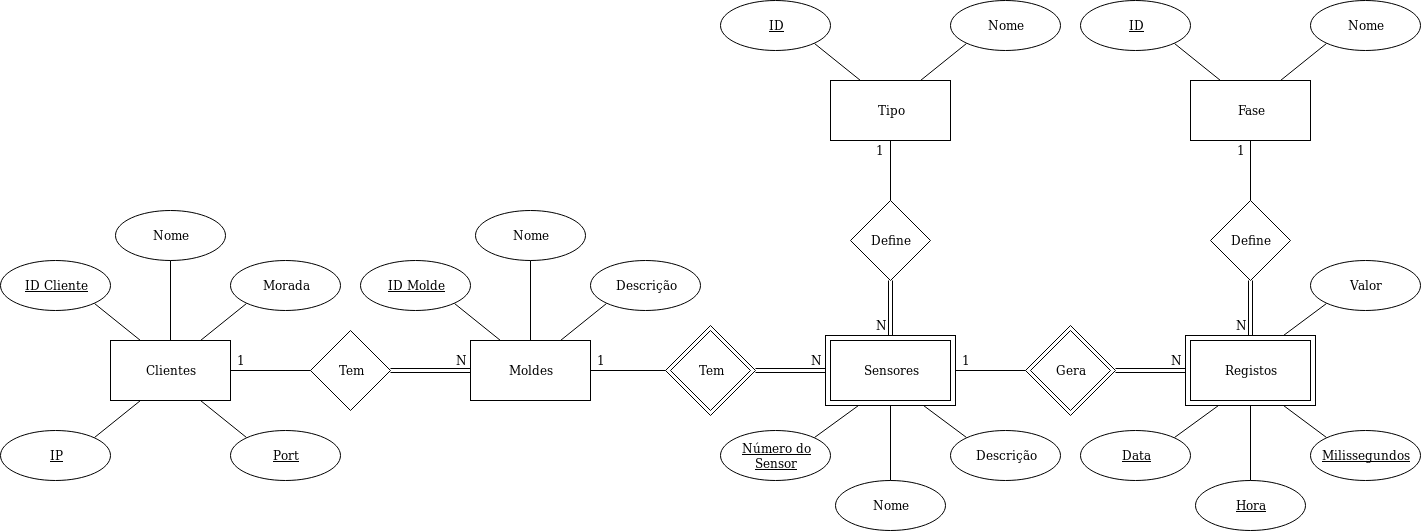
\includegraphics[width=1.4\textwidth]{diagrama_entidade_relacao} % Include the image placeholder.png
			\caption[Diagrama Entidade/Relação final do projeto]{Diagrama Entidade/Relação final do projeto realizado a partir da análise de requisitos}
			\label{fig:der}
		\end{center}
	\end{figure}
\end{landscape}
\subsection{Desenho conceptual e esquema lógico}
Concatenando a informação descrita na análise de requisitos, obtém-se o diagrama entidade/relação representado na \autoref{fig:der}.\par
Traduzindo as entidades do diagrama anterior para tabelas e as relações para chaves estrangeiras, obtém-se o esquema lógico da base de dados representado na \autoref{fig:er}.
\begin{figure}[H]
	\begin{center}
		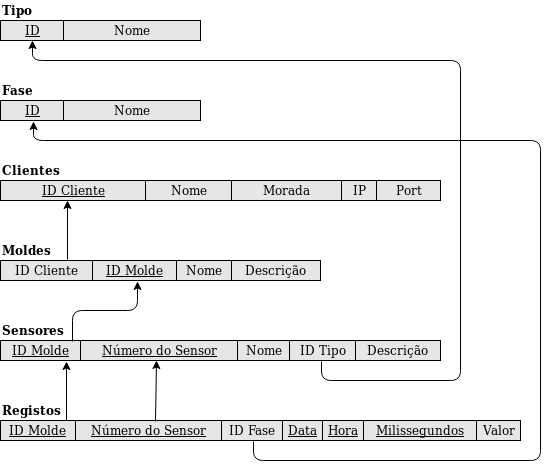
\includegraphics[width=1\textwidth]{esquema_relacional} % Include the image placeholder.png
		\caption[Esquema Lógico final do projeto]{Esquema Lógico final do projeto obtido através da análise do diagrama entidade/relação na \autoref{fig:der} onde as entidades e os seus atributos se traduzem em tabelas e as relações nas chaves estrangeiras destas}
		\label{fig:er}
	\end{center}
\end{figure}

\newpage
\subsection{Construção da base de dados}
Avançando para a criação das tabelas em \textit{MySQL}, a fim de evitar ambiguidades no nome dos atributos estes são alterados para campos semânticos específicos a cada entidade a que pertencem. Para cada atributo define-se o domínio e a obrigatoriedade como representado na \autoref{tab:dominio}.
\begin{table}[H]
	\centering
	\begin{tabular}{|l|l|l|l|l|l|}
		%\hline
		\multicolumn{6}{l}{\textbf{tipo}}\\ \cline{1-2}
		tipo\texttt{\char`_}ID & tipo\texttt{\char`_}nome & \multicolumn{4}{l}{}\\ \cline{1-2}
		int & varchar(50) & \multicolumn{4}{l}{}\\ \cline{1-2}
		not null & not null & \multicolumn{4}{l}{}\\ \cline{1-2}
		\multicolumn{6}{l}{\textbf{fase}}\\ \cline{1-2}
		fase\texttt{\char`_}ID & fase\texttt{\char`_}nome & \multicolumn{4}{l}{}\\ \cline{1-2}
		int & varchar(50) & \multicolumn{4}{l}{}\\ \cline{1-2}
		not null & not null & \multicolumn{4}{l}{}\\ \cline{1-2}
		\multicolumn{6}{l}{\textbf{clientes}}\\ \cline{1-5}
		cl\texttt{\char`_}ID & cl\texttt{\char`_}nome & cl\texttt{\char`_}morada & cl\texttt{\char`_}IP & cl\texttt{\char`_}port & \multicolumn{1}{l}{}\\ \cline{1-5}
		int & varchar(50) & varchar(100) & varchar(50) & int & \multicolumn{1}{l}{}\\ \cline{1-5}
		not null & not null & & not null & not null & \multicolumn{1}{l}{}\\ \cline{1-5}
		\multicolumn{6}{l}{\textbf{moldes}}\\ \cline{1-4}
		m\texttt{\char`_}IDCliente & m\texttt{\char`_}ID & 
		m\texttt{\char`_}nome & 
		m\texttt{\char`_}descricao & \multicolumn{2}{l}{}\\ \cline{1-4}
		int & int & varchar(30) & varchar(200) & \multicolumn{2}{l}{}\\ \cline{1-4}
		not null & not null & & &  \multicolumn{2}{l}{}\\ \cline{1-4}
		\multicolumn{6}{l}{\textbf{sensores}}\\ \cline{1-5}
		s\texttt{\char`_}IDMolde & s\texttt{\char`_}num & s\texttt{\char`_}tipo & s\texttt{\char`_}nome & s\texttt{\char`_}descricao & \multicolumn{1}{l}{}\\ \cline{1-5}
		int & int & int & varchar(30) & varchar(200) & \multicolumn{1}{l}{}\\ \cline{1-5}
		not null & not null & not null & & & \multicolumn{1}{l}{}\\ \cline{1-5}
		\multicolumn{6}{l}{\textbf{registos}}\\ \hline
		r\texttt{\char`_}IDMolde & r\texttt{\char`_}numSensor & r\texttt{\char`_}fase &  r\texttt{\char`_}data\texttt{\char`_}hora & r\texttt{\char`_}milissegundos & r\texttt{\char`_}valor\\ \hline
		int & int & int & datetime & tinyint & float\\ \hline
		not null & not null & not null & not null & not null & \\ \hline
	\end{tabular}
	\caption[Tabelas das bases de dados com os seus atributos e respetivos domínios e obrigatoriedades]{Tabelas das bases de dados com os seus atributos e respetivos domínios e obrigatoriedades. Os atributos data e hora da entidade registos são fundidos no atributo r\texttt{\char`_}data\texttt{\char`_}hora graças ao tipo de dados datetime}
	\label{tab:dominio}
\end{table}
Define-se então nomes para as restrições de integridade definidas pelas chaves das entidades:
\begin{itemize}[noitemsep]
	\item Tipo
	\begin{itemize}[noitemsep]
		\item Restrição chave primária: REPETIDO\texttt{\char`_}ID\texttt{\char`_}TIPO
		\item Restrição chaves únicas:
		\begin{enumerate}
			\item REPETIDO\texttt{\char`_}NOME\texttt{\char`_}TIPO
		\end{enumerate}
	\end{itemize}
	\item Fase
	\begin{itemize}[noitemsep]
		\item Restrição chave primária: REPETIDO\texttt{\char`_}ID\texttt{\char`_}FASE
		\item Restrição chaves únicas:
		\begin{enumerate}
			\item REPETIDO\texttt{\char`_}NOME\texttt{\char`_}FASE
		\end{enumerate}
	\end{itemize}
	\item Clientes
	\begin{itemize}[noitemsep]
		\item Restrição chave primária: REPETIDO\texttt{\char`_}ID\texttt{\char`_}CLIENTE
	\end{itemize}
	\item Moldes
	\begin{itemize}[noitemsep]
		\item Restrição chave primária: REPETIDO\texttt{\char`_}ID\texttt{\char`_}MOLDE
		\item Restrição chaves estrangeiras:
		\begin{enumerate}
			\item MOLDE\texttt{\char`_}MAU\texttt{\char`_}ID\texttt{\char`_}CLIENTE
		\end{enumerate}
	\end{itemize}
	\item Sensores
	\begin{itemize}[noitemsep]
		\item Restrição chave primária: REPETIDO\texttt{\char`_}NUM\texttt{\char`_}SENSOR
		\item Restrição chaves estrangeiras:
		\begin{enumerate}
			\item SENSOR\texttt{\char`_}MAU\texttt{\char`_}ID\texttt{\char`_}MOLDE
			\item SENSOR\texttt{\char`_}MAU\texttt{\char`_}ID\texttt{\char`_}TIPO
		\end{enumerate}
	\end{itemize}
	\item Registos
	\begin{itemize}[noitemsep]
		\item Restrição chave primária: REPETIDO\texttt{\char`_}REGISTO
		\item Restrição chaves estrangeiras:
		\begin{enumerate}
			\item REGISTOS\texttt{\char`_}MAU\texttt{\char`_}ID\texttt{\char`_}MOLDE\texttt{\char`_}SENSOR
			\item REGISTOS\texttt{\char`_}MAU\texttt{\char`_}ID\texttt{\char`_}FASE
		\end{enumerate}
	\end{itemize}
\end{itemize}
Em relação ao comportamento das restrições das chaves estrangeiras identificam-se as seguintes opções:
\begin{itemize}
	\item ON DELETE NO ACTION ON UPDATE NO ACTION
	\begin{itemize}
		\item MOLDE\texttt{\char`_}MAU\texttt{\char`_}ID\texttt{\char`_}CLIENTE
		\item SENSOR\texttt{\char`_}MAU\texttt{\char`_}ID\texttt{\char`_}TIPO
		\item REGISTOS\texttt{\char`_}MAU\texttt{\char`_}ID\texttt{\char`_}FASE
	\end{itemize}
	\item ON DELETE CASCADE ON UPDATE NO ACTION
	\begin{itemize}
		\item SENSOR\texttt{\char`_}MAU\texttt{\char`_}ID\texttt{\char`_}MOLDE
		\item REGISTOS\texttt{\char`_}MAU\texttt{\char`_}ID\texttt{\char`_}MOLDE\texttt{\char`_}SENSOR
	\end{itemize}
\end{itemize}
Estes comportamentos definem que quando se tenta atualizar a chave primária de um tuplo (\textit{UPDATE}), se esta tiver tuplos associados a ela, a operação não deve ser realizada pois pode comprometer os dados existentes na base de dados. No entanto, quando se tenta eliminar um tuplo são definidos dois comportamentos. Como existe muita informação associada a cada cliente, como segurança, não se permite a eliminação de um tuplo desta tabela se este tiver informação associada a si noutras tabelas. O mesmo se aplica aos dicionários, se se tentar eliminar um tuplo, a informação associada não deve ser comprometida. No caso dos registos, dado que estão associados diretamente a um molde, se um tuplo da tabela moldes for eliminado, os dados dos seus sensores e respetivos registos devem ser também eliminados para manter a base de dados limpa e sem informação desnecessária.\par 
\newpage
Revendo as restrições de integridade criadas pelas chaves estrangeiras, como não se pode criar uma tabela que dependa de outra que não tenha sido ainda criada, define-se uma ordem para a criação das tabelas:
\begin{enumerate}[noitemsep]
	\item Tipo
	\item Fase
	\item Clientes
	\item Moldes
	\item Sensores
	\item Registos
\end{enumerate}
Este modelo de dados aplica-se a todas as bases de dados usadas neste projeto com a exceção da base de dados regulação de procedimentos abordada na \autoref{subchap:notificacoes} e temporária local abordada na \autoref{subchap:adap}.

\subsection{Base de dados regulação de procedimentos}
\label{subchap:notificacoes}
Com a introdução da aplicação de gestão do sistema surge a necessidade desta comunicar com os programas de transferência e gestão de \textit{backups}. Para este efeito cria-se a base de dados regulação de procedimentos, com a qual a aplicação comunica de forma a ditar o modo de funcionamento dos programas, como representado na \autoref{fig:infra4}.
\begin{figure}[H]
	\centering
	\begin{center}
		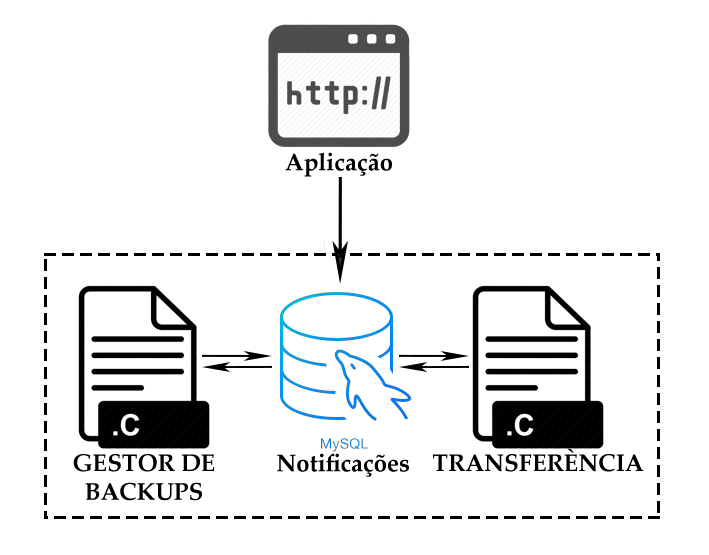
\includegraphics[width=0.5\textwidth]{Aplicacao_notificacoes} % Include the image placeholder.png
		\caption[Diagrama da comunicação com a base de dados regulação de procedimentos]{Diagrama da comunicação com a base de dados regulação de procedimentos, onde os programas de transferência e gestão de \textit{backups} verificam parâmetros introduzidos pela aplicação}
		\label{fig:infra4}
	\end{center}
\end{figure}
Esta base de dados contém variáveis globais importantes para a comunicação entre a aplicação e os programas. Define-se as entidades com os seus atributos e respetivos domínios e obrigatoriedade como representado na \autoref{tab:notificacoes}. As entidades não se relacionam entre e por isso esta base de dados não se classifica como uma base de dados relacional. No entanto, utiliza-se os mesmos termos para descrever o desenvolvimento desta.
\begin{table}[H]
	\centering
	\begin{tabular}{|l|l|}
		%\hline
		\multicolumn{2}{l}{\textbf{atualizar}}\\ \cline{1-2}
		a\texttt{\char`_}transferencia & a\texttt{\char`_}backups\\ \cline{1-2}
		int & int\\ \cline{1-2}
		not null & not null\\ \cline{1-2}
		\multicolumn{2}{l}{\textbf{backups}}\\ \cline{1-1}
		b\texttt{\char`_}IDMolde &\multicolumn{1}{l}{}\\ \cline{1-1}
		int &\multicolumn{1}{l}{}\\ \cline{1-1}
		 &\multicolumn{1}{l}{}\\ \cline{1-1}
	\end{tabular}
	\caption[Tabelas da base de dados regulação de procedimentos com os seus atributos e respetivos domínios e obrigatoriedades]{Tabela base de dados regulação de procedimentos com os seus atributos e respetivos domínios e obrigatoriedades}
	\label{tab:notificacoes}
\end{table}
A tabela Atualizar só deve ter um tuplo e os valores dos atributos \texttt{a\char`_transferencia} e \texttt{a\char`_backups} só devem ser 0 ou 1. Assim sendo definem-se as restrições:
\begin{itemize}[noitemsep]
	\item Atualizar
	\begin{itemize}[noitemsep]
		\item Restrição valor:
		\begin{enumerate}
			\item MAU\texttt{\char`_}VALOR\texttt{\char`_}TRANSFERENCIA
			\item MAU\texttt{\char`_}VALOR\texttt{\char`_}BACKUPS
		\end{enumerate}
	\end{itemize}
	\item Backups
	\begin{itemize}[noitemsep]
		\item Restrição chaves únicas:
		\begin{enumerate}
			\item REPETIDO\texttt{\char`_}ID\texttt{\char`_}MOLDE
		\end{enumerate}
	\end{itemize}
\end{itemize}
Define-se que tabela Atualizar deve ser iniciada com um tuplo onde os seus atributos são iguais a 0. As funcionalidades desta base de dados são exploradas nas Secções \ref{subchap:transferencia} e \ref{subchap:backups}.

\section{Programa de transferência}
\label{subchap:transferencia}
Este programa prioriza a conservação dos dados e a sua taxa de transferência. O código foi realizado com vista à portabilidade para outras linguagens de programação. Consiste em várias ideias simples que podem ser observadas nas Figuras \ref{fig:transferencia_programa} e \ref{fig:transferencia_subprograma}.\par 
\begin{figure}
	\vspace{-3cm}
	\begin{center}
		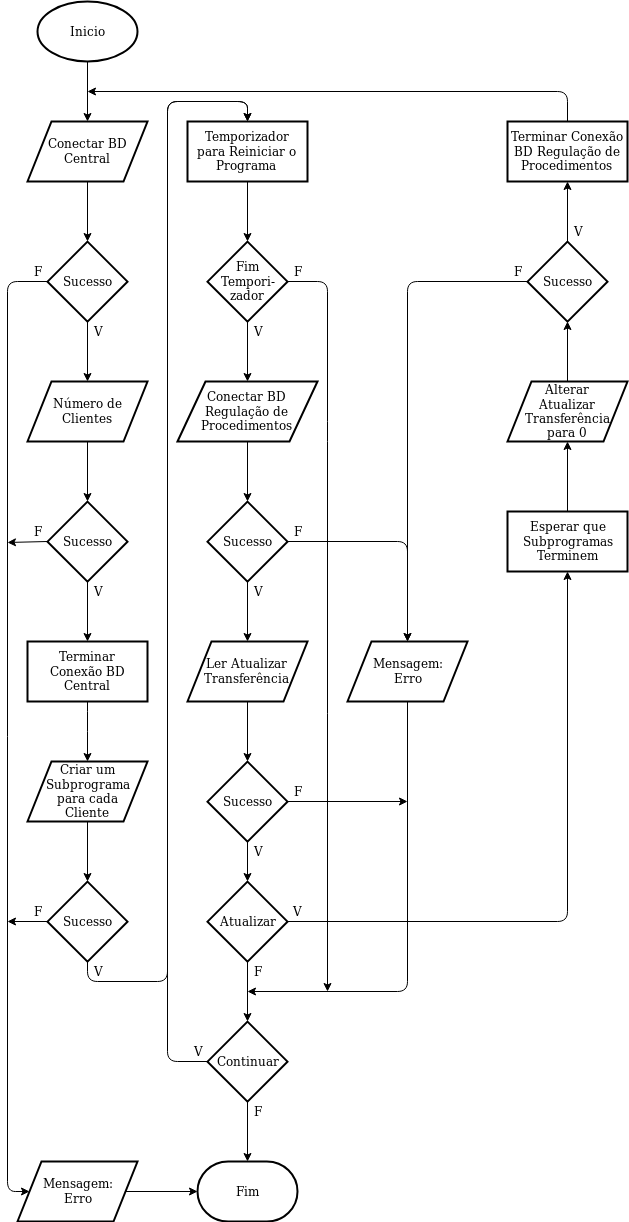
\includegraphics[width=.75\textwidth]{fluxograma_transferencia_programa4} % Include the image placeholder.png
		%\vspace{9cm}
		\caption{Fluxograma do programa principal que cria os subprogramas}
		\label{fig:transferencia_programa}
	\end{center}
\end{figure}
\begin{figure}
	\begin{center}
		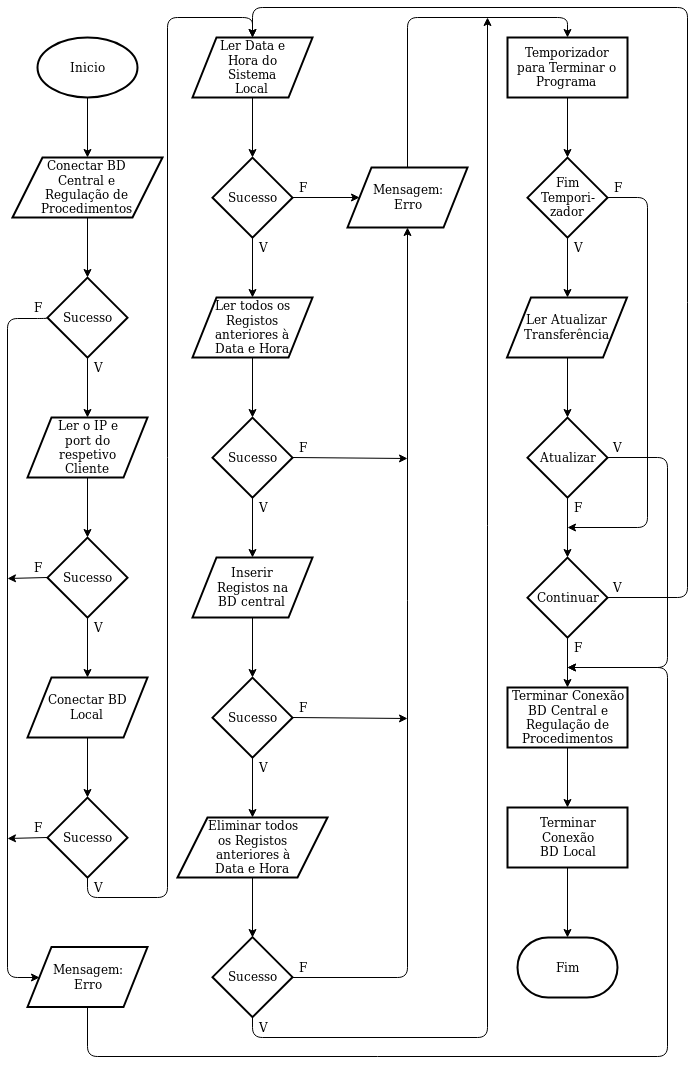
\includegraphics[width=0.85\textwidth]{fluxograma_transferencia_subprograma4} % Include the image placeholder.png
		\caption{Fluxograma dos subprogramas criados para transferirem registos de cada cliente para a base de dados central}
		\label{fig:transferencia_subprograma}
	\end{center}
\end{figure}
Seguindo a estrutura do programa, primeiramente realiza-se uma conexão à base de dados central, seguida de uma \textit{query} para se saber o número de clientes existentes:
\begin{lstlisting}[language = SQL]
	SELECT *
	FROM clientes;
\end{lstlisting}
Guarda-se o número de tuplos retornados numa variável e termina-se a conexão à base de dados central. De seguida replica-se o programa múltiplas vezes até se ter um subprograma para cada cliente com recurso à função:
\begin{lstlisting}[language = C]
	fork();
\end{lstlisting}
Atribui-se a cada subprograma o número do cliente a que está associado. Cada um realiza uma conexão à base de dados central e obtém os respetivos \textit{IPs} e \textit{ports}, necessários para realizar a conexão à base de dados local de cada cliente:
\begin{lstlisting}[language = SQL]
	SELECT cl_ID, cl_IP, cl_port
	FROM clientes
	ORDER BY cl_ID;
\end{lstlisting}
Com as conexões central e local estabelecidas inicia-se um ciclo infinito para a transferência de valores. Com a \textit{query} à base de dados local:
\begin{lstlisting}[language = SQL]
	SELECT CURRENT TIMESTAMP;
\end{lstlisting}
Recebe-se a data e hora atual do sistema e guarda-se numa variável \texttt{@datahora\char`_lim}. De seguida obtém-se todos os registos anteriores à data e hora do sistema:
\begin{lstlisting}[language = SQL]
	SELECT *
	FROM registos
	WHERE r_data_hora < @datahora_lim
	ORDER BY r_data_hora, r_milissegundos,
	r_numSensor, r_IDMolde;
\end{lstlisting}
Esta organização pela data e hora garante uma transferência uniforme de valores. Por predefinição, o sistema retorna os registos um sensor de cada vez, tornando a transferência de valores menos eficiente para efeitos de análise. Por outras palavras, prefere-se saber os registos de todos os sensores num dado instante do que todos os registos de um sensor até ao momento. Os tuplos retornados são guardados numa \textit{string} e inseridos na base de dados central com uma \textit{query} do tipo:
\begin{lstlisting}[language = SQL]
	INSERT IGNORE registos VALUES
	(tuplo1),
	(tuplo2),
	(tuplo3),
	...,
	(tuploN);
\end{lstlisting}
Inserir múltiplos tuplos permite uma maior taxa de transferência comparativamente a uma inserção individual. A \textit{string} que guarda os tuplos tem uma dimensão limitada, se a resposta proveniente da base de dados local for superior ao tamanho da \textit{string}, o programa divide-a em grupos de informação mais pequenos que respeitem a dimensão desta \textit{string}. A escolha da opção \texttt{IGNORE} garante que não são perdidos valores no caso de serem gerados registos repetidos ou não válidos. Após a transferência ser concluída, os tuplos transferidos da base de dados local são eliminados:
\begin{lstlisting}[language = SQL]
	DELETE FROM registos
	WHERE r_data_hora < @datahora_lim;
\end{lstlisting}
Sempre que se desejar um subprograma para um cliente novo, o programa de transferência deve ser reiniciado. Isto pode ser realizado manualmente ou atualizando o valor de \texttt{a\char`_transferencia} para 1. Com base num temporizador o programa principal e os subprogramas realizam a \textit{query} à base de dados regulação de procedimentos:
\begin{lstlisting}[language = SQL]
	SELECT a_transferencia
	FROM atualizar;
\end{lstlisting}
Se \texttt{@a\char`_transferencia} for igual a 1 os subprogramas terminam após completarem os seus ciclos e o programa principal recomeça do principio como demonstrado nas Figuras \ref{fig:transferencia_programa} e \ref{fig:transferencia_subprograma}.

\section{Gestão de \textit{backups}}
\label{subchap:backups}
À semelhança do programa anterior, o programa de gestão de \textit{backups} foi realizado com vista à portabilidade para outras linguagens de programação. Este programa está dividido nas componentes de gerar e concatenar de \textit{backups}.\par 
A primeira serve para manter a informação armazenada organizada. Gera \textit{backups} segmentados dos históricos de registos da base de dados central e depois elimina a informação já salvaguardada. Isto aumenta a velocidade de consulta de registos mais recentes e previne que a base de dados central exceda o limite de 4Gb impostos pela versão gratuita do \textit{MySQL}, como referido na \autoref{subchap:mysql}. Em vez de se gerar um \textit{backup} de toda a base de dados, gera-se um \textit{backup} específico para cada molde, que inclui a informação dos seus sensores, registos e cliente a que está associado. Além destes, realiza-se um outro \textit{backup} com a informação dos clientes, moldes e sensores mais atual. Assim, em caso de falha crítica, simplifica-se a recuperação do sistema. A segunda serve para concatenar os \textit{backups} segmentados, produzidos durante o tempo de funcionamento de um molde, num \textit{backup} total do histórico de registos do molde. Quando um molde sai de produção pode ser interessante arquivar o seu histórico e esta ação pode ser facilitada se, em vez de serem arquivados dezenas ou centenas de \textit{backups}, for apenas arquivado um \textit{backup} geral com todo o histórico do molde.\par 
Ao contrário do programa anterior, este programa não executa de forma contínua. Define-se um temporizador para executar cada componente. Utilizam-se temporizadores diferentes um maior e outro mais pequeno. O temporizador maior porque a primeira componente executa automaticamente e, dependendo do que for definido, em intervalos espaçados. Por exemplo: uma vez por dia ou por semana ou por mês dependendo da quantidade de informação produzida. O temporizador menor porque a segunda componente executa quando o utilizador deseja e deve garantir uma resposta do programa com o menor de latência possível.
As Figuras \ref{fig:backups_programa}, \ref{fig:backups_gerar} e \ref{fig:backups_concatenar} representam a estrutura do programa.\par 
\begin{figure}
	\begin{center}
		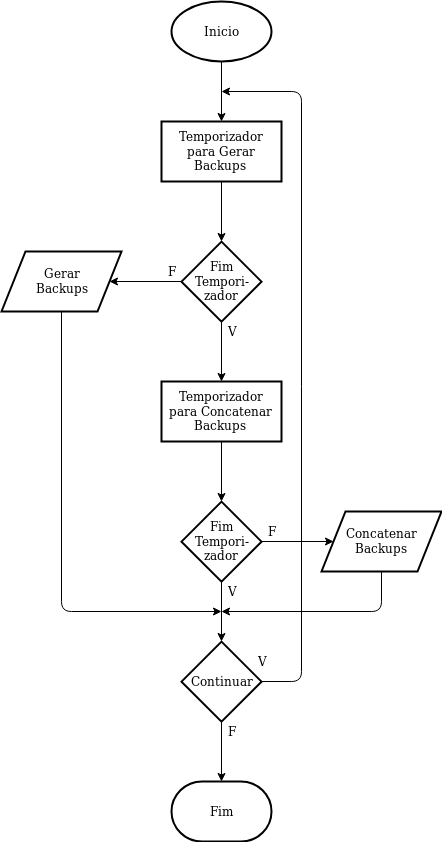
\includegraphics[width=0.7\textwidth]{fluxograma_backups_programa01} % Include the image placeholder.png
		\caption{Fluxograma do programa principal com os temporizadores para gerar ou concatenar \textit{backups}}
		\label{fig:backups_programa}
	\end{center}
\end{figure}
\begin{figure}
	\begin{center}
		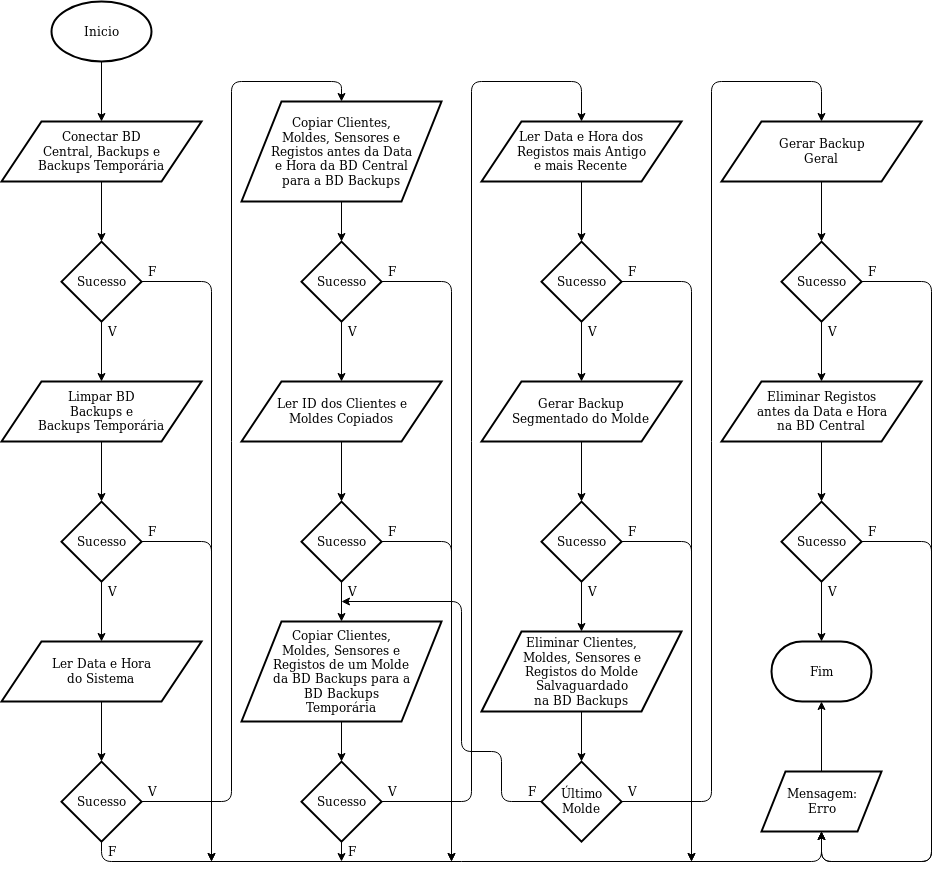
\includegraphics[width=1\textwidth]{fluxograma_backups_gerar01} % Include the image placeholder.png
		\caption[Fluxograma da componente de gerar \textit{backups}]{Fluxograma da componente de gerar \textit{backups}. Quando esta chega ao fim retorna ao ciclo do programa principal representado na \autoref{fig:backups_programa}}
		\label{fig:backups_gerar}
	\end{center}
\end{figure}
\begin{figure}
	\begin{center}
		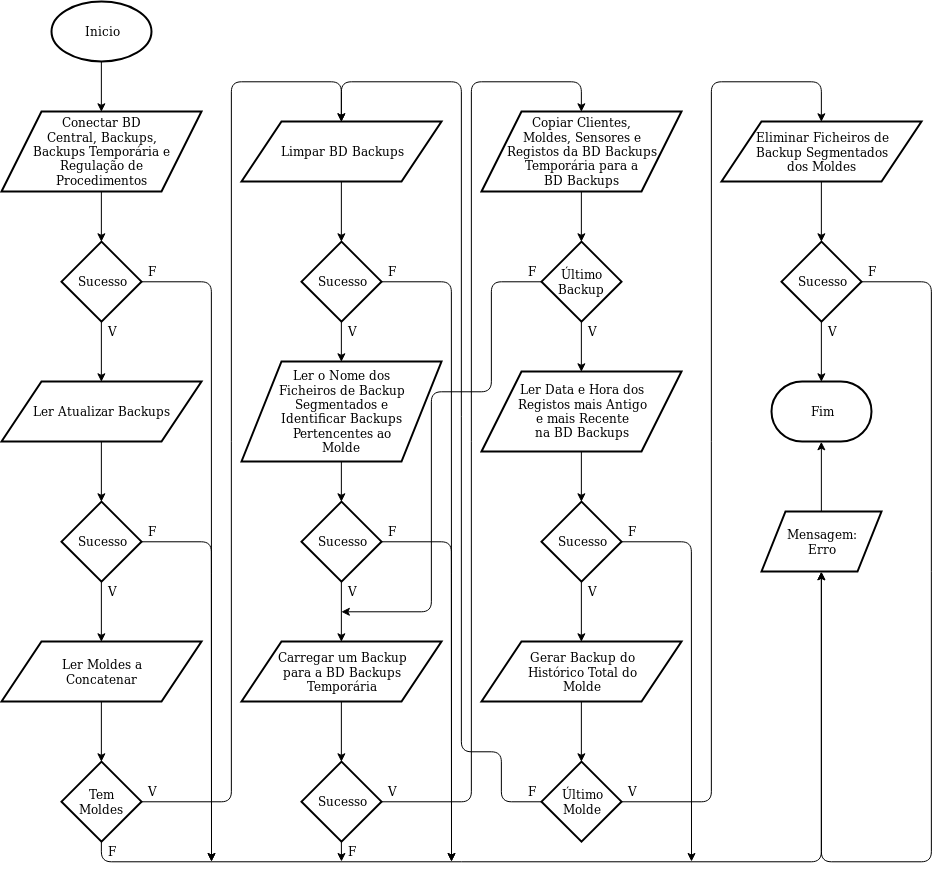
\includegraphics[width=1\textwidth]{fluxograma_backups_concatenar01} % Include the image placeholder.png
		\caption[Fluxograma da componente de concatenar \textit{backups}]{Fluxograma da componente de concatenar \textit{backups}. Quando esta chega ao fim retorna ao ciclo do programa principal representado na \autoref{fig:backups_programa}}
		\label{fig:backups_concatenar}
	\end{center}
\end{figure}
\newpage
Seguindo a estrutura da componente de geração de \textit{backups} representado na \autoref{fig:backups_gerar}, realizam-se as conexões às bases de dados central, \textit{backups} e \textit{backups} temporária.  Realiza-se uma limpeza da base de dados \textit{backups} e \textit{backups} temporária para certificar que não existem valores que possam comprometer a informação dos \textit{backups}:
\begin{lstlisting}[language = SQL]
	DELETE FROM backups.moldes;
	DELETE FROM backups.clientes;
	DELETE FROM backups_temp.moldes;
	DELETE FROM backups_temp.clientes;
\end{lstlisting}
Com a \textit{query}:
\begin{lstlisting}[language = SQL]
	SELECT CURRENT TIMESTAMP;
\end{lstlisting}
Recebe-se a data e hora atual do sistema e guarda-se numa variável \texttt{@datahora\char`_lim}. Para proteger os dados presentes na base de dados central, realiza-se a cópia dos registos para a base de dados \textit{backups}:
\begin{lstlisting}[language = SQL]
	INSERT IGNORE backups.clientes
	SELECT *
	FROM central.clientes;
	INSERT IGNORE backups.moldes
	SELECT *
	FROM central.moldes;
	INSERT IGNORE backups.sensores
	SELECT *
	FROM central.sensores;
	INSERT IGNORE backups.registos
	SELECT *
	FROM central.registos
	WHERE r_data_hora < @datahora_lim;
\end{lstlisting}
De forma a gerar um \textit{backup} para cada molde filtra-se a informação com base no seu ID:
\begin{lstlisting}[language = SQL]
	SELECT m_IDCliente, m_ID
	FROM backups.moldes;
\end{lstlisting}
As respostas são guardadas nas variáveis \texttt{@IDCliente} e \texttt{@IDMolde}. De forma cíclica copia-se a informação para a base de dados \textit{backups} temporária:
\begin{lstlisting}[language = SQL]
	INSERT IGNORE backups_temp.clientes
	SELECT *
	FROM backups.clientes
	WHERE cl_ID = @IDCliente;
	INSERT IGNORE backups_temp.moldes
	SELECT *
	FROM backups.moldes
	WHERE m_ID = @IDMolde;
	INSERT IGNORE backups_temp.sensores
	SELECT *
	FROM backups.sensores
	WHERE m_ID = @IDMolde;
	INSERT IGNORE backups_temp.registos
	SELECT *
	FROM backups.registos
	WHERE m_ID = @IDMolde;
\end{lstlisting}
Após os valores copiados retiram-se informações sobre a data e hora mais antiga e mais recente:
\begin{lstlisting}[language = SQL]
	SELECT r_data_hora
	FROM backups_temp.registos
	ORDER BY r_data_hora
	LIMIT 1;
	SELECT r_data_hora
	FROM backups_temp.registos
	ORDER BY r_data_hora DESC
	LIMIT 1;
\end{lstlisting}
Os valores retornados são guardados nas variáveis \texttt{@dataIni} e \texttt{@dataFim}. Com estes valores e com a função:
\begin{lstlisting}[language = C]
	FILE *popen(const char *command, const chat *mode);
\end{lstlisting}
Envia-se para o terminal o comando que gera os \textit{backups} num local predefinido:
\begin{lstlisting}[language = bash]
	mysqldump -u backupmanager -pbackup1234 backups_temp >
	~/Backups/backup_@IDCliente_@IDMolde_@dataIni_@dataFim.sql
\end{lstlisting}
Depois do ficheiro ser criado com sucesso elimina-se das bases de dados \textit{backups} e \textit{backups} temporária a informação relativa ao molde:
\begin{lstlisting}[language = SQL]
	DELETE FROM backups_temp.moldes;
	DELETE FROM backups_temp.clientes;
	DELETE FROM bakups.registos
	WHERE r_IDMolde = @IDMolde;
\end{lstlisting}
Quando todos os moldes tiverem sido armazenados, a tabela registos da base de dados \textit{backups} deve estar vazia. Realiza-se então o \textit{backup} da restante informação dos clientes, moldes, sensores, tipo e fase para efeitos de recuperação do sistema:
\begin{lstlisting}[language = bash]
	mysqldump -u backupmanager -pbackup1234 backups_temp >
	~/Backups/backup_geral.sql
\end{lstlisting}
Definiu-se um nome estático para este \textit{backup}. Este será rescrito cada vez que o programa executa enquanto os \textit{backups} individuais dos moldes vão acumulando com o tempo. Termina-se o processo apagando os valores armazenados na base de dados central:
\begin{lstlisting}[language = SQL]
	DELETE FROM central.registos
	WHERE r_data_hora < @datahora_lim;
\end{lstlisting}
Os \textit{backups} são então transferidos para o repositório \textit{online} no \textit{GitHub}. Esta solução serve apenas para demonstrar a capacidade de mover os \textit{backups} para um sistema diferente. Do ponto de vista prático, não se recomenda guardar informação potencialmente sensível num servidor público.\par 
Na eventualidade de surgir uma falha crítica no sistema central, e este necessitar de ser formatado ou substituído, os registos cessarão de ser transferidos dos sistemas locais. Isto não significa que a informação esteja comprometida, apenas não está a ser transferida. Após re-instalar utiliza-se manualmente no terminal o comando:
\begin{lstlisting}[language = bash]
	mysql -u backupmanager -pbackup1234 central <
	~/Backups/backup_geral.sql
\end{lstlisting}
Isto faz com que se recupere a informação dos clientes, moldes e sensores presentes no último \textit{backup} de forma a acelerar o processo de restauro comparativamente a uma inserção manual dos dados.\par 
Passando para a componente de concatenação de \textit{backups}, os ficheiros criados com o comando \texttt{mysqldump} contêm toda a informação das tabelas e funcionam como ponto de restauro. Isto significa que quando se usa o comando de recuperação, a base de dados selecionada é substituída pela que está no ficheiro \texttt{.sql}. Este comportamento dificulta a concatenação de vários \textit{backups} numa única base de dados assim sendo, à semelhança da primeira componente, utiliza-se a base de dados \textit{backups} temporária como base de dados intermédia para a concatenação de \textit{backups}.\par 
Seguindo a estrutura do programa representada na \autoref{fig:backups_concatenar}, realizam-se as conexões às bases de dados central, \textit{backups}, \textit{backups} temporária e regulação de procedimentos. Com a \textit{query}:
\begin{lstlisting}[language = SQL]
	SELECT a_backups
	FROM regulacao_procedimentos.atualizar;
\end{lstlisting}
Retira-se o parâmetro \texttt{@a\char`_backups}, se este for igual a 1 o programa tem de concatenar \textit{backups}. Identificam-se os moldes a ser arquivados:
\begin{lstlisting}[language = SQL]
	SELECT b_IDMolde
	FROM regulacao_procedimentos.backups;
\end{lstlisting}
As respostas são guardadas numa variável \texttt{@IDMolde}. Realiza-se uma limpeza da base de dados \textit{backups} para certificar que não existem valores que possam comprometer a informação dos \textit{backups}:
\begin{lstlisting}[language = SQL]
	DELETE FROM backups.moldes;
	DELETE FROM backups.clientes;
\end{lstlisting}
Identificam-se os \textit{backups} referentes ao molde e, de forma cíclica, carregam-se os ficheiros na base de dados \textit{backups} temporária:
\begin{lstlisting}[language = bash]
	mysql -u backupmanager -pbackup1234 backups_temp <
	~/Backups/backup_IDCliente_@IDMolde_dataIni_dataFim.sql
\end{lstlisting}
E copia-se a informação para a base de dados \textit{backups}:
\begin{lstlisting}[language = SQL]
	INSERT IGNORE backups.clientes
	SELECT *
	FROM backups_temp.clientes;
	INSERT IGNORE backups.moldes
	SELECT *
	FROM backups_temp.moldes;
	INSERT IGNORE backups.sensores
	SELECT *
	FROM backups_temp.sensores;
	INSERT IGNORE backups.registos
	SELECT *
	FROM backups_temp.registos;
\end{lstlisting}
Após os valores carregados e copiados para a base de dados \textit{backups} retiram-se informações sobre o cliente, a data e hora mais antiga e mais recente:
\begin{lstlisting}[language = SQL]
	SELECT r_data_hora
	FROM backups.registos
	ORDER BY r_data_hora
	LIMIT 1;
	SELECT r_data_hora
	FROM backups.registos
	ORDER BY r_data_hora DESC
	LIMIT 1;
\end{lstlisting}
Estes valores são guardados nas variáveis \texttt{@IDCliente}, \texttt{@dataIni} e \texttt{@dataFim}. Gera-se então o \textit{backup} total do histórico completo do molde:
\begin{lstlisting}[language = bash]
	mysqldump -u backupmanager -pbackup1234 backups >
	~/Backups/Arquivo/
	backup_@IDCliente_@IDMolde_@dataIni_@dataFim.sql
\end{lstlisting}
Com este \textit{backup} gerado deixa de ser necessário manter os \textit{backups} segmentados e procede-se à eliminação destes. Estes operações executam de forma cíclica até todos os moldes selecionados serem arquivados.

\section{Simulador}
Para popular as bases de dados locais foi desenvolvido um simples programa que gera valores. Estes seguem o perfil de uma onda sinusoidal com a expressão:
\begin{equation}
v = O + A\sin(\frac{2 \pi x}{t} + \gamma)
\label{eq:sim1}
\end{equation}
Onde \textit{v} é o valor calculado, \textit{O} o \textit{offset} da onda, \textit{A} a amplitude, \textit{t} o período em segundos, \textit{x} a hora atual em segundos e $ \gamma $ o desfasamento. Inicia-se uma conexão à base de dados local e calcula-se a hora atual com recurso às funções:
\begin{lstlisting}[language = C]
	struct tm *localtime(const time_t *timer);
	int gettimeofday(struct timeval *tv, struct timezone *tz);
\end{lstlisting}
Os valores das horas, minutos, segundos e milissegundos são guardados nas variáveis \texttt{@hora}, \texttt{@min}, \texttt{@seg} e \texttt{@mseg} respetivamente. Aplicando a expressão:
\begin{equation}
x = @hora \times 3600 + @min \times 60 + @seg + @mseg \times 0.001
\label{eq:sim2}
\end{equation}
Obtém-se a hora atual do sistema em segundos. Com as expressões \ref{eq:sim1} e \ref{eq:sim2} gera-se um valor para cada sensor. Para cada valor gerado atribuí-se uma fase do processo. Esta atribuição realiza-se de forma cíclica entre as várias opções disponíveis. Com a informação de cada sensor estabelecida insere-se na base de dados local com uma \textit{query} do estilo:
\begin{lstlisting}[language = SQL]
	INSERT INTO registos VALUES
	(molde1, sensor1, fase, NOW(), @mseg, valor11),
	(molde1, sensor2, fase, NOW(), @mseg, valor12),
	(molde2, sensor1, fase, NOW(), @mseg, valor21),
	...,
	(moldeI, sensorN, fase, NOW(), @mseg, valorIN);
\end{lstlisting}

\section{Utilizadores}
Para minimizar o risco de erros por parte dos utilizadores que interagem com o sistema, são definidas credenciais com permissões específicas para cada base de dados:
\begin{itemize}[noitemsep]
	\item user, password
	\item transferencia, transferencia1234
	\item sensores, sensores1234
	\item backupmanager, backup1234
\end{itemize}
\textit{user} representa o utilizador padrão, ou seja, aquele que interage com as bases de dados para gerir os clientes, moldes e sensores bem como consultar a tabela registos. As credenciais \textit{transferencia} utilizam-se no programa de transferência de valores para realizar as conexões com as bases de dados central e locais, \textit{sensores} utiliza-se no simulador para popular as bases de dados locais e, no futuro, pelo sistema de aquisição de dados que substituirá este simulador, \textit{backupmanager} utiliza-se no programa de gestão de \textit{backups}.\par 
Cada conjunto de credenciais serve um objetivo, a \autoref{tab:utilizadores1} contém as permissões destas definidas em cada base de dados.\par 
\begin{table}
	\begin{tabular}{|l|c|c|c|c|c|c|}
		%\hline
		\multicolumn{7}{l}{\textbf{central}} \\ \hline
		\makecell{clientes/tipo/fase/\\moldes/sensores} & CREATE & DROP & SELECT & INSERT & DELETE & UPDATE \\ \hline
		user & & & \textbf{X} & \textbf{X} & \textbf{X} & \textbf{X} \\ \hline
		transferencia & & & & & & \\ \hline
		sensores & & & & & & \\ \hline
		backupmanager & & & \textbf{X} & & & \\ \hline
		registos & CREATE & DROP & SELECT & INSERT & DELETE & UPDATE \\ \hline
		user & & & \textbf{X} & & \textbf{X} & \\ \hline
		transferencia & & & & \textbf{X} & & \\ \hline
		sensores & & & & & & \\ \hline
		backupmanager & & & \textbf{X} & & \textbf{X} & \\ \hline
		\multicolumn{7}{l}{\textbf{local}} \\ \hline
		\makecell{clientes/tipo/fase/\\moldes/sensores} & CREATE & DROP & SELECT & INSERT & DELETE & UPDATE \\ \hline
		user & & & \textbf{X} & \textbf{X} & \textbf{X} & \textbf{X} \\ \hline
		transferencia & & & & & & \\ \hline
		sensores & & & & & & \\ \hline
		backupmanager & & & & & & \\ \hline
		registos & CREATE & DROP & SELECT & INSERT & DELETE & UPDATE \\ \hline
		user & & & & & & \\ \hline
		transferencia & & & \textbf{X} & & \textbf{X} & \\ \hline
		sensores & & & & \textbf{X} & & \\ \hline
		backupmanager & & & & & & \\ \hline
		\multicolumn{7}{l}{\textbf{\textit{backups} e \textit{backups} temporária}} \\ \hline
		\makecell{clientes/tipo/\\fase/moldes/\\sensores/registos} & CREATE & DROP & SELECT & INSERT & DELETE & UPDATE \\ \hline
		user & & & & & & \\ \hline
		transferencia & & & & & & \\ \hline
		sensores & & & & & & \\ \hline
		backupmanager & & & \textbf{X} & \textbf{X} & \textbf{X} & \\ \hline
		\multicolumn{7}{l}{\textbf{regulação de procedimentos}} \\ \hline
		\makecell{atualizar} & CREATE & DROP & SELECT & INSERT & DELETE & UPDATE \\ \hline
		user & & & \textbf{X} & & & \textbf{X} \\ \hline
		transferencia & & & \textbf{X} & & & \textbf{X} \\ \hline
		sensores & & & & & & \\ \hline
		backupmanager & & & \textbf{X} & & & \textbf{X} \\ \hline
		backups & CREATE & DROP & SELECT & INSERT & DELETE & UPDATE \\ \hline
		user & & & \textbf{X} & \textbf{X} & \textbf{X} & \textbf{X} \\ \hline
		transferencia & & & & & & \\ \hline
		sensores & & & & & & \\ \hline
		backupmanager & & & \textbf{X} & & \textbf{X} & \\ \hline
	\end{tabular}
	\caption{Tabelas com as permissões das credenciais criadas para as várias tabelas das bases de dados}
	\label{tab:utilizadores1}
\end{table}
Estas permissões estabelecem que nenhuma das credenciais estabelecidas pode fazer DROP às bases de dados o que eliminaria com um comando toda a estrutura e a informação nela contida. Além disto, nenhuma tem permissão INSERT e DELETE simultânea na tabela registos das bases de dados central e local protegendo o sistema de adulteração dos valores presentes nesta tabela.

\cleardoublepage
\chapter{Aplicação de Gestão do Sistema}
\label{chap:aplicacao}
A aplicação foi desenvolvida em ambiente  \textit{Web} com o objetivo de ser multiplataforma e permitir acesso remoto e sem recorrer a instalação de \textit{softwares} nos dispositivos dos utilizadores. Corre num servidor \textit{Apache} e foi desenvolvida com \textit{PHP}, \textit{JS} e \textit{HTML}. Este capítulo descreve a adaptação da infraestrutura desenvolvida e as várias funcionalidades da aplicação.

\section{Adaptação da infraestrutura}
\label{subchap:adap}
A infraestrutura desenvolvida no \autoref{chap:solucao} visa uma utilização a baixo a nível. Ainda que funcional, pode haver margem para erros e incoerência dos dados introduzidos manualmente. A aplicação minimiza estas incoerências através da instalação de uma nova base de dados temporária local no servidor local. Aqui os utilizadores têm a liberdade para adicionar, alterar e apagar informação sem consequências no sistema antes desta ser introduzida nas bases de dados central e local como representado na \autoref{fig:adap1}. Como referido anteriormente, esta base de dados difere das restantes, não contendo em si as tabelas fase e registos.
\begin{figure}[H]
	\begin{center}
		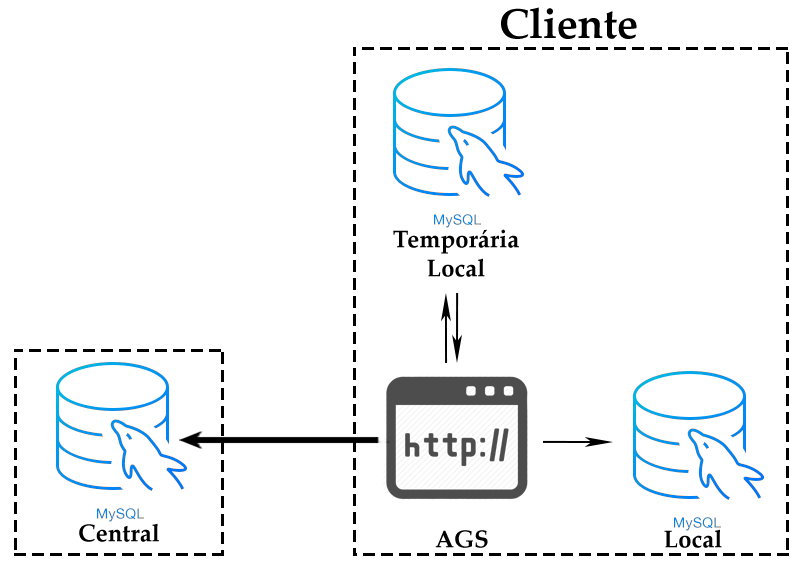
\includegraphics[width=0.62\textwidth]{Aplicacao_temp_local_central} % Include the image placeholder.png
		\caption{Esquema ligação Aplicação-Bases de Dados. A aplicação comunica com a base de dados temporária local e depois regista os seus valores nas bases de dados central e local}
		\label{fig:adap1}
	\end{center}
\end{figure}

\section{Interface gráfica}
A aplicação divide-se em quatro partes distintas:
\begin{itemize}[noitemsep]
	\item \textit{Main} - Página principal
	\item \textit{Login} - Página de acesso
	\item Consultas
	\item Administração Local
\end{itemize}
As páginas \textit{Main}, \textit{Login} e Consultas realizadas para uma utilização geral. A página Administração Local foi realizada para uma utilização local. A primeira visa um uso a partir de qualquer dispositivo e acessível a qualquer momento e a segunda foca-se num acesso local com o objetivo de configurar e definir a informação no servidor local. Por outras palavras, para o utilizador usar as funcionalidades desta página tem de aceder à aplicação num \textit{browser} no sistema local que se situa no cliente.\par 
Instalar um molde é o culminar de um projeto de elevada responsabilidade e esta ideia junto com a criação da base de dados temporária local serve para melhorar a qualidade da informação introduzida no sistema e diminuir as falhas no processo de instalação deste.

\newpage
\subsection{\textit{Main}}
\begin{figure}[H]
\centering
	\begin{minipage}{1.\textwidth}
		\begin{center}
			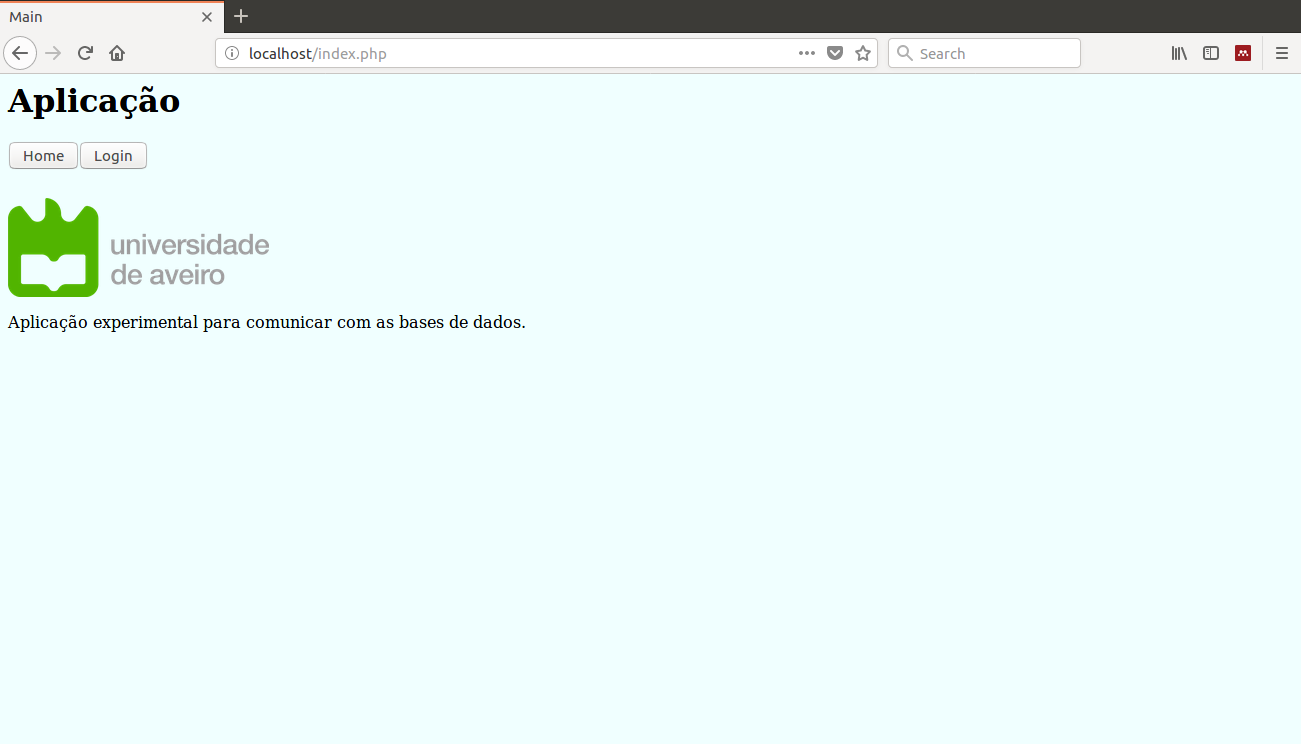
\includegraphics[width=0.85\textwidth]{main01} % Include the image placeholder.png
			\subcaption{Sem \textit{login}}
			\label{fig:main1}
		\end{center}
	\end{minipage}
	\begin{minipage}{1.\textwidth}
		\begin{center}
			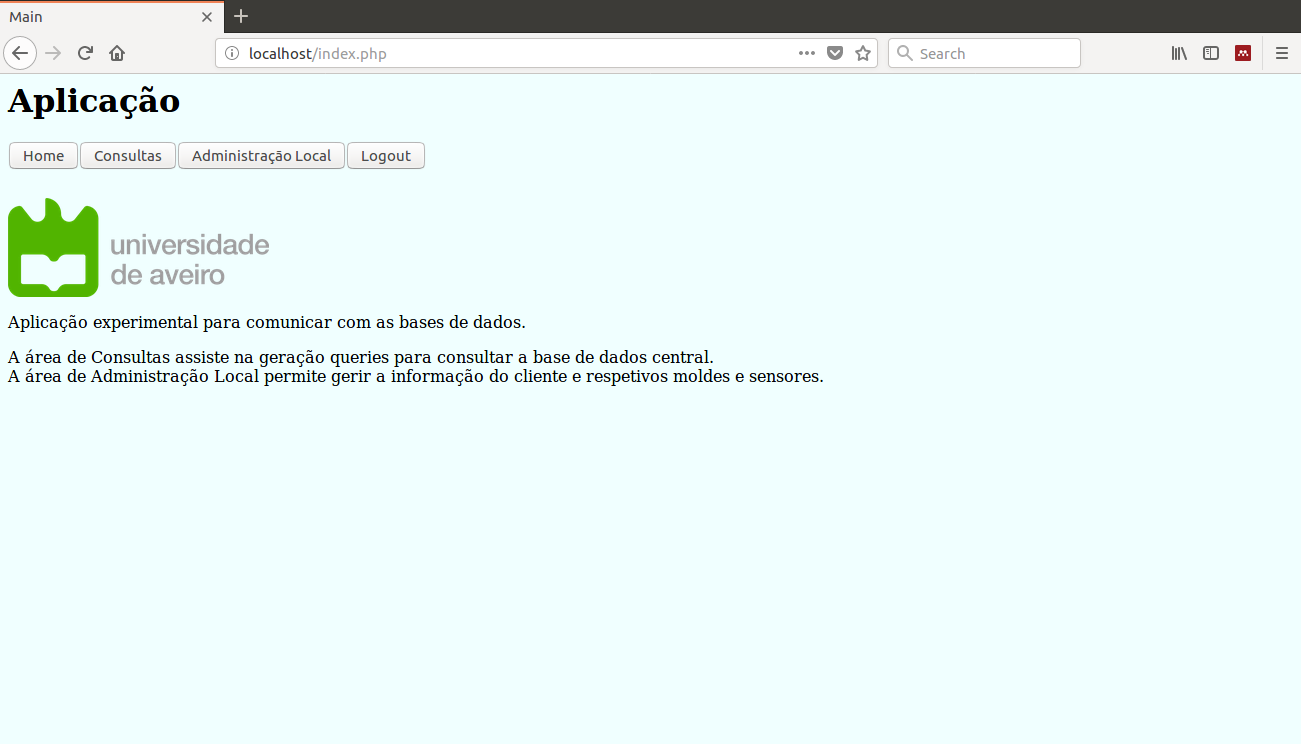
\includegraphics[width=0.85\textwidth]{main02} % Include the image placeholder.png
			\subcaption{Com \textit{login}}
			\label{fig:main2}
		\end{center}
	\end{minipage}
	\caption{Funcionalidades da página \textit{Main} com e sem \textit{login}}
	\label{fig:main0}
\end{figure}
\textit{Main} serve como página principal da aplicação. Se não houver sessão iniciada, todas as restantes páginas redirecionam o utilizador para aqui. Contém apenas algumas informações gerais sobre a aplicação.\par 
Iniciar sessão na página de \textit{Login} desbloqueia funcionalidades na aplicação, como demonstrado nas Figuras \ref{fig:main1} e \ref{fig:main2}. Depois de iniciada a sessão, navega-se com os botões para as páginas de Consultas e Administração Local.

\subsection{\textit{Login}}
\begin{figure}[H]
	\begin{center}
		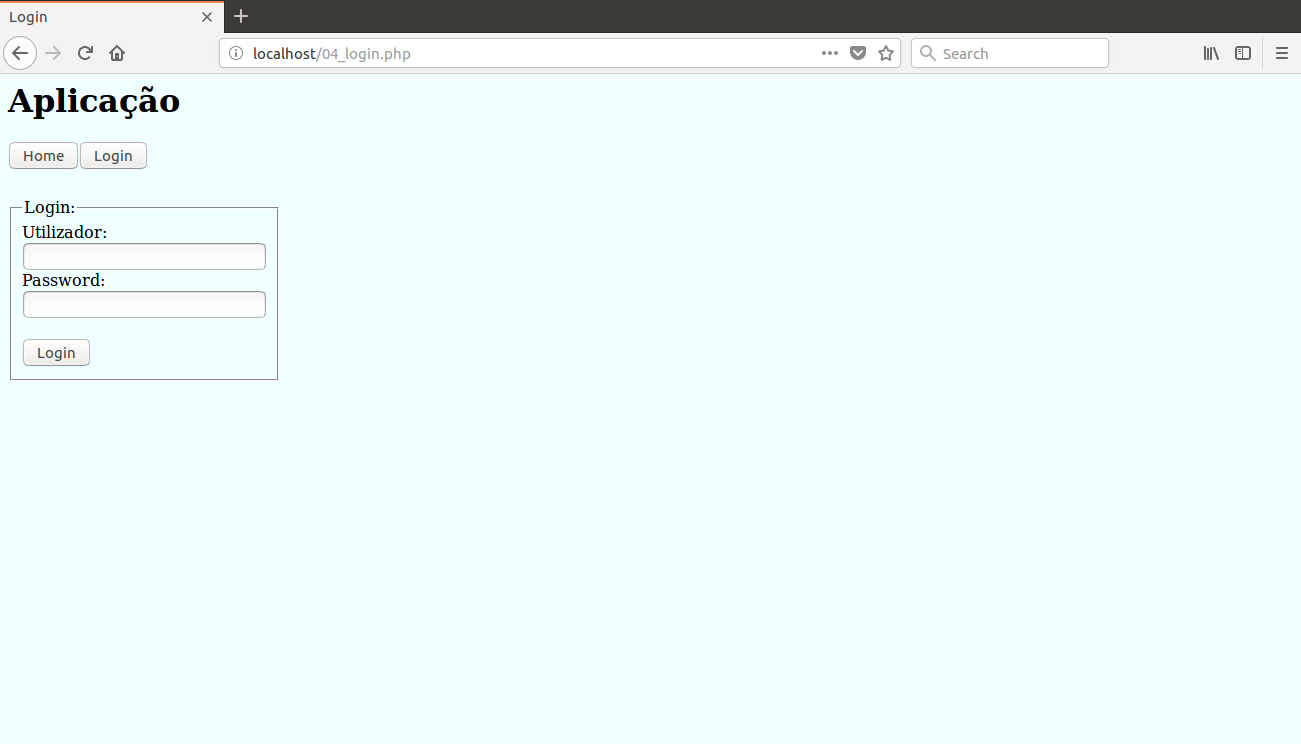
\includegraphics[width=0.9\textwidth]{login01} % Include the image placeholder.png
		\caption{Página de \textit{Login} para iniciar sessão na base de dados central}
		\label{fig:login0}
	\end{center}
\end{figure}
A página de \textit{Login} consiste num simples formulário constituído por duas caixas de texto e um botão, como demonstrado na \autoref*{fig:login0}. O botão \textit{Login} lê as credenciais introduzidas e realiza uma conexão de teste à base de dados central validando-as diretamente com \textit{MySQL}. Se as credenciais forem validadas com sucesso redireciona-se o utilizador para a página principal e altera-se o botão de \textit{Login} para \textit{Logout}. Se as credenciais introduzidas não forem suficientes ou válidas são retornados erros de forma a informar o utilizador como demonstrado nas Figuras \ref{fig:login2} e \ref{fig:login3}.\par 
Quando se acede à página com \textit{Logout} termina-se a sessão e redireciona-se o utilizador para a página principal.
\begin{figure}[H]
	\centering
	\begin{minipage}{.5\textwidth}
		\begin{center}
			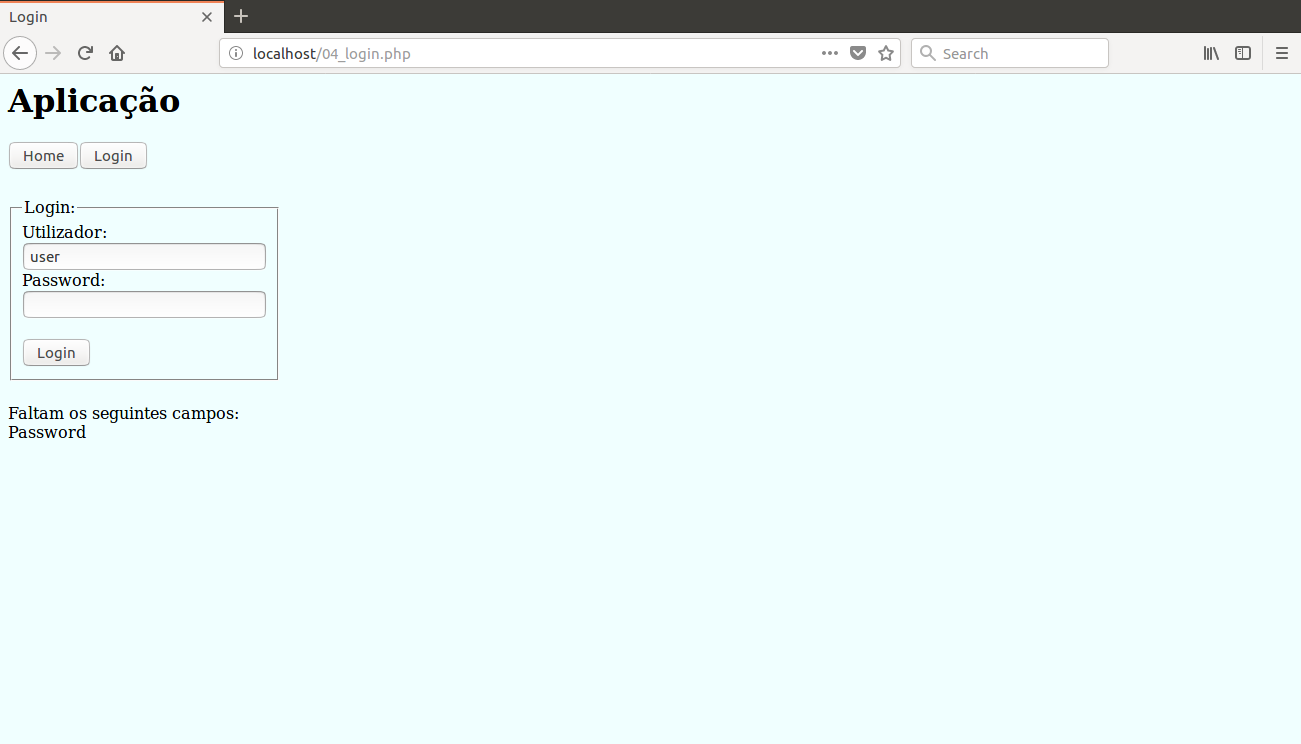
\includegraphics[width=0.95\textwidth]{login02} % Include the image placeholder.png
			\subcaption{Exemplo de erro de falta de informação}
			\label{fig:login2}
		\end{center}
	\end{minipage}%
	\begin{minipage}{.5\textwidth}
		\begin{center}
			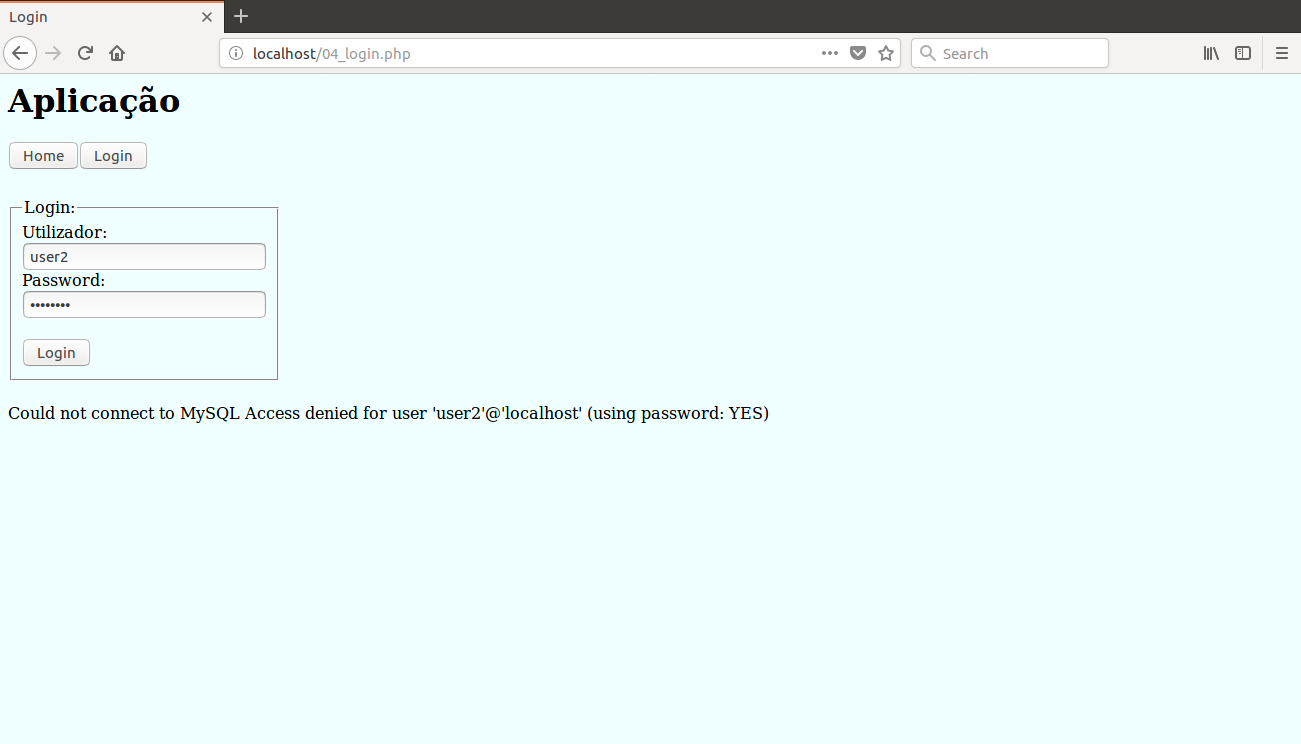
\includegraphics[width=0.95\textwidth]{login03} % Include the image placeholder.png
			\subcaption{Exemplo de erro \textit{MySQL}}
			\label{fig:login3}
		\end{center}
	\end{minipage}
	\caption{Exemplos de erros retornados quando introduzidas credenciais não válidas na página \textit{Login}}
	\label{fig:login1}
\end{figure}

\subsection{Consultas}
\begin{figure}[H]
	\centering
	\begin{minipage}{1.\textwidth}
		\begin{center}
			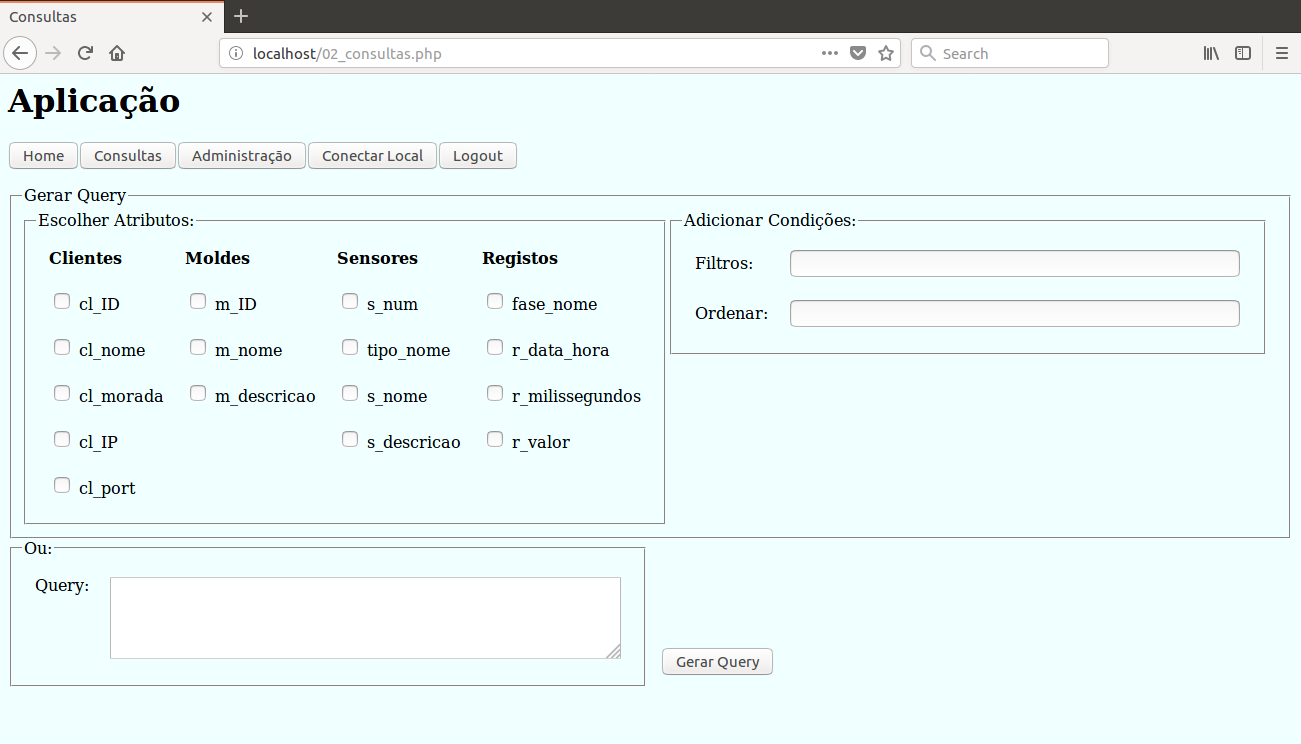
\includegraphics[width=.9\textwidth]{consultas01} % Include the image placeholder.png
			\subcaption{Página de Consultas}
			\label{fig:consultas1}
		\end{center}
	\end{minipage}
	\begin{minipage}{1.\textwidth}
		\begin{center}
			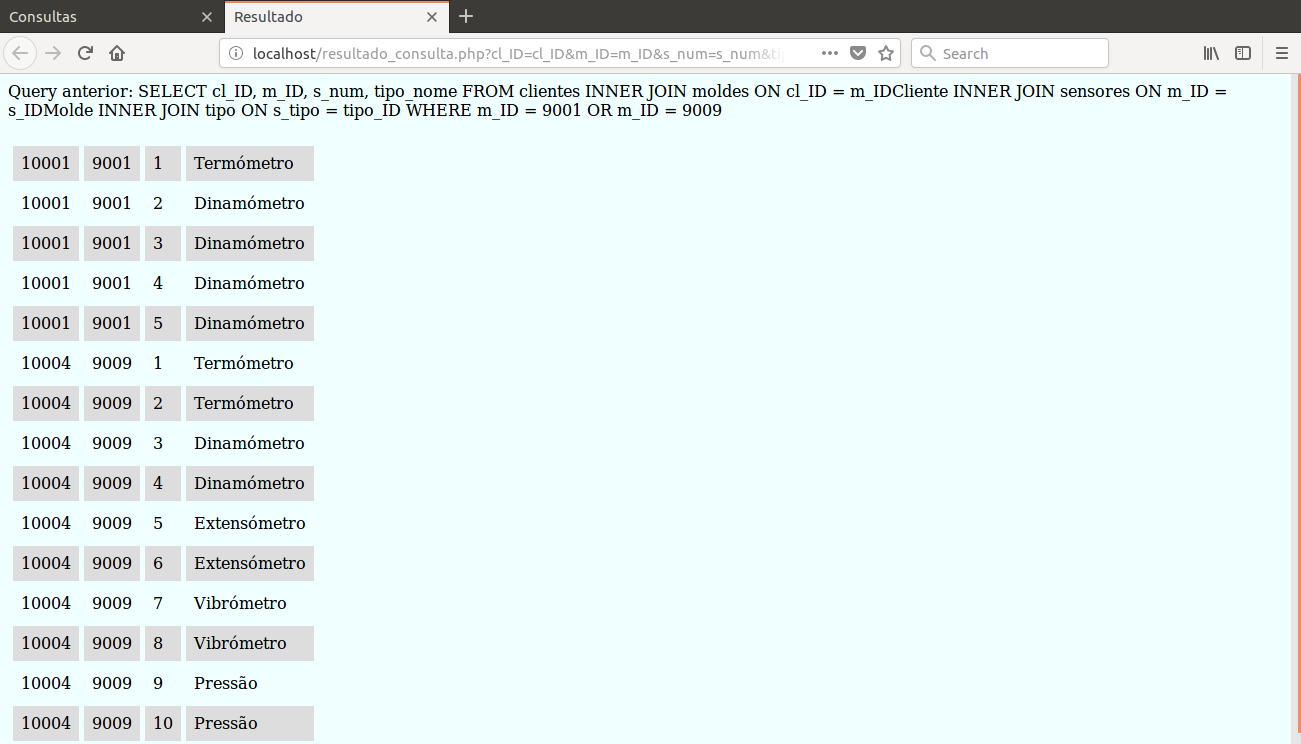
\includegraphics[width=0.9\textwidth]{consultas02} % Include the image placeholder.png
			\subcaption{Exemplo de resposta de consulta}
			\label{fig:consultas2}
		\end{center}
	\end{minipage}
	\caption{Página de Consultas e exemplo de resposta a uma consulta}
	\label{fig:consultas0}
\end{figure}
A página de Consultas assiste os utilizadores sem conhecimentos de \textit{SQL} a criarem \textit{queries} para consultar a base de dados central. Na \autoref{fig:consultas1} observa-se várias \textit{checkboxes} e três caixas de texto. As \textit{checkboxes} permitem selecionar os atributos que se desejam consultar na base de dados; estes atributos são guardados numa variável \texttt{@atributos}.
\newpage
Quando  se prime o botão \textit{Query} gera-se uma das seguintes quatro \textit{queries}:
\begin{lstlisting}[language = SQL]
1-	SELECT @atributos
	FROM clientes;
	
2-	SELECT @atributos
	FROM clientes
	INNER JOIN moldes ON cl_ID = m_IDCliente;
	
3-	SELECT @atributos
	FROM clientes
	INNER JOIN moldes ON cl_ID = m_IDCliente
	INNER JOIN sensores ON m_ID = s_IDMolde
	INNER JOIN tipo ON s_tipo = tipo_ID;
	
4-	SELECT @atributos FROM clientes
	INNER JOIN moldes ON cl_ID = m_IDCliente
	INNER JOIN sensores ON m_ID = s_IDMolde 
	INNER JOIN tipo ON s_tipo = tipo_ID
	INNER JOIN registos ON s_IDMolde = r_IDMolde
	AND s_num = r_numSensor
	INNER JOIN fase ON r_fase = fase_ID;
\end{lstlisting}
A seleção é feita com base na coluna mais à esquerda a que os atributos pertencem. Explicando melhor com um exemplo: se o utilizador desejar consultar o \texttt{cl\char`_ID} e o \texttt{cl\char`_nome} da tabela clientes gera-se a primeira \textit{query} no entanto, se o utilizador desejar consultar os atributos \texttt{cl\char`_ID}, \texttt{m\char`_ID} e \texttt{s\char`_num} gera-se a terceira \textit{query}.\par
Além destas, foram adicionadas três \textit{queries} especificas quando os atributos \texttt{tipo\char`_}nome, \texttt{fase\char`_nome} e \texttt{r\char`_data}\texttt{\char`_hora} são selecionados sozinhos. As primeiras duas permitem consultar as opções disponíveis nos dicionários e a terceira devolve as datas e horas entre o primeiro e último registos.\par
As caixas de texto Filtros e Ordem na \autoref{fig:consultas1} permitem adicionar às \textit{queries} geradas as cláusulas WHERE e ORDER BY, respetivamente. Para os utilizadores com conhecimentos em \textit{SQL} está disponibilizada a caixa de texto \textit{Query} que permite a criação direta de uma \textit{query}. Este campo está limitado apenas para \textit{queries} do tipo SELECT.\par
Depois da \textit{query} ser gerada retorna-se uma resposta num novo separador como demonstrado na \autoref{fig:consultas2}. O \textit{link} desta resposta contém toda a informação da \textit{query} gerada. Este pode ser arquivado ou enviado para outro utilizador sem ser necessário gerar a \textit{query} novamente, isto é útil para \textit{queries} com muitas cláusulas.\par
Se a \textit{query} não for válida retorna-se um erro de forma a informar o utilizador, como demonstrado nas Figuras \ref{fig:consultas4}, \ref{fig:consultas5} e \ref{fig:consultas6}.
\newpage
\begin{figure}[H]
	\centering
	\begin{minipage}{1\textwidth}
		\begin{center}
			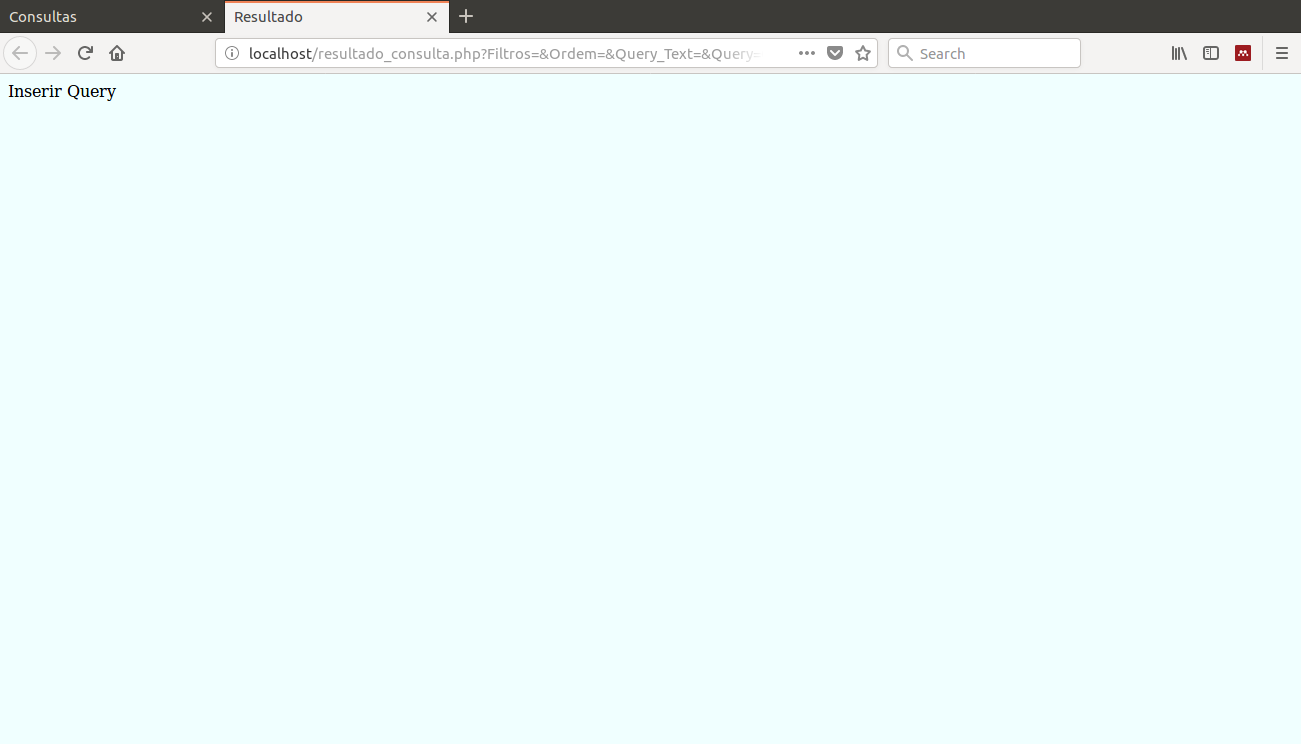
\includegraphics[width=0.7\textwidth]{consultas03} % Include the image placeholder.png
			\subcaption{Erro de informação não introduzida}
			\label{fig:consultas4}
		\end{center}
	\end{minipage}
	\begin{minipage}{1\textwidth}
		\begin{center}
			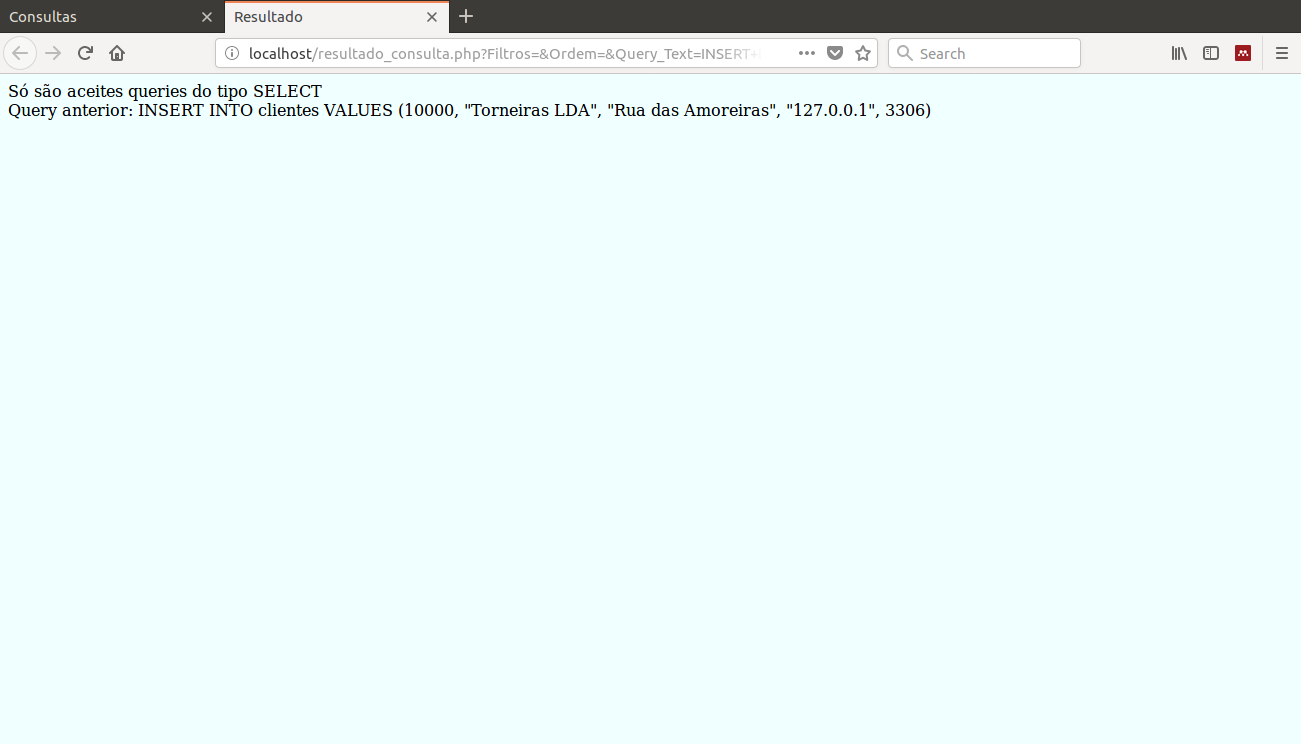
\includegraphics[width=0.7\textwidth]{consultas04} % Include the image placeholder.png
			\subcaption{Erro de \textit{query} que não é do tipo SELECT}
			\label{fig:consultas5}
		\end{center}
	\end{minipage}
	\begin{minipage}{1\textwidth}
		\begin{center}
			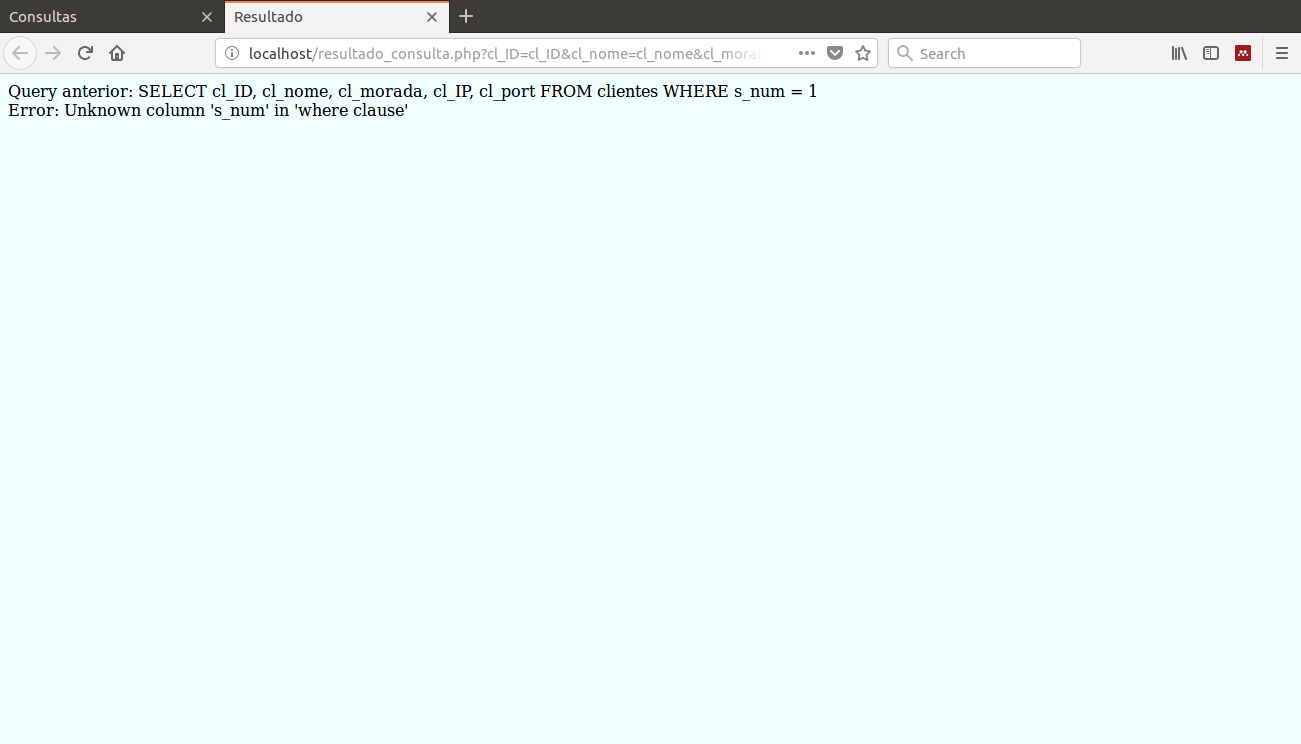
\includegraphics[width=0.7\textwidth]{consultas05} % Include the image placeholder.png
			\subcaption{Exemplo de erro \textit{MySQL}}
			\label{fig:consultas6}
		\end{center}
	\end{minipage}
	\caption{Exemplos de erros retornados na página de Resposta da Consulta}
	\label{fig:consultas3}
\end{figure}

\subsection{Administração Local}
\begin{figure}[H]
	\centering
	\begin{minipage}{1\textwidth}
		\begin{center}
			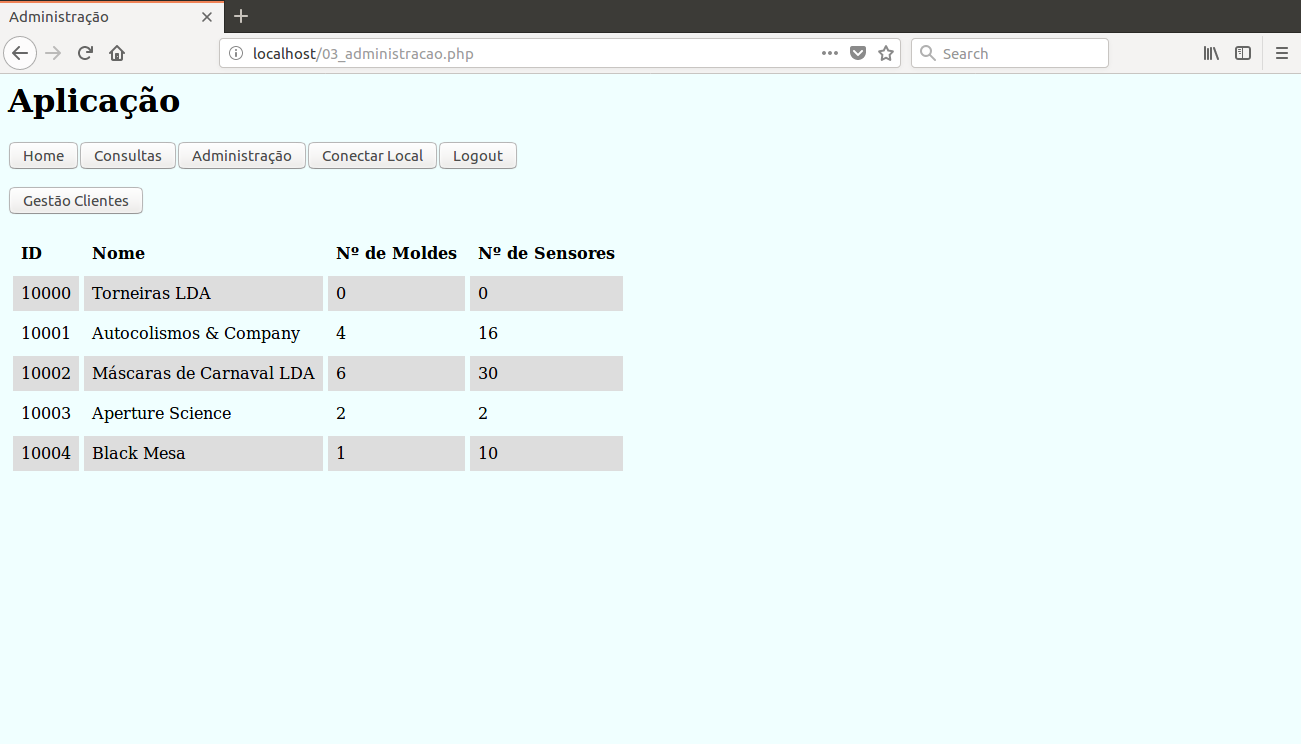
\includegraphics[width=0.9\textwidth]{administracao01} % Include the image placeholder.png
			\subcaption{Sem conexão local}
			\label{fig:admin1}
		\end{center}
	\end{minipage}
	\begin{minipage}{1\textwidth}
		\begin{center}
			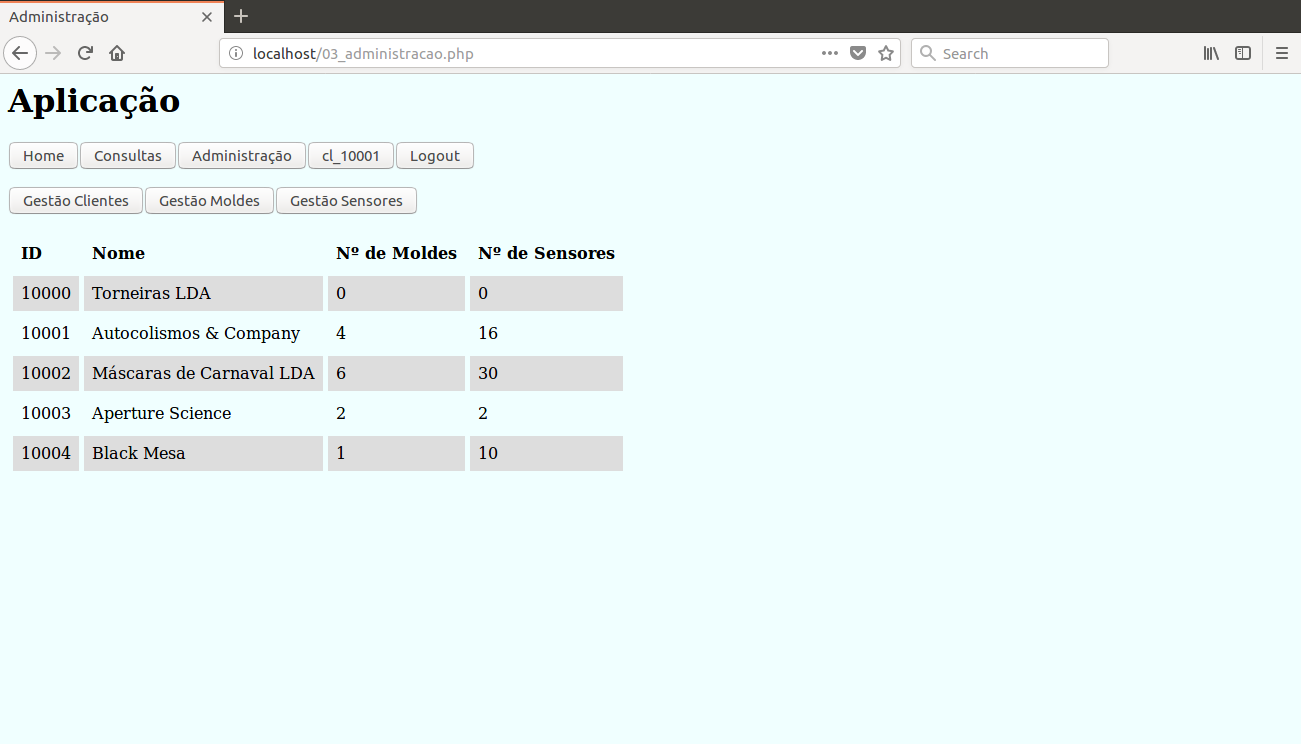
\includegraphics[width=0.9\textwidth]{administracao03} % Include the image placeholder.png
			\subcaption{Com conexão local}
			\label{fig:admin2}
		\end{center}
	\end{minipage}
	\caption{Funcionalidades da página Administração com e sem conexão local}
	\label{fig:admin0}
\end{figure}
Esta área está dividida em duas componentes distintas. A componente de Administração permite ao utilizador alterar informações sobre os clientes, moldes e sensores. A componente de Conectar Local permite realizar uma conexão à base de dados local no servidor do cliente. A componente de Administração só pode ser acedida quando for efetuada uma conexão local. Após a conexão ser bem sucedida observa-se informação do cliente com a \textit{query}:
\begin{lstlisting}[language = SQL]
	SELECT cl_ID, cl_nome, COUNT(DISTINCT m_ID),
	COUNT(DISTINCT s_IDMolde, s_num)
	FROM clientes LEFT OUTER JOIN moldes ON cl_ID = m_IDCliente
	LEFT OUTER JOIN sensores ON m_ID = s_IDMolde
	GROUP BY cl_ID;
\end{lstlisting}

\subsubsection{Administração}
Esta componente está dividida em três áreas: Gestão de Clientes, Gestão de Moldes e Gestão de Sensores como demonstrado na \autoref{fig:admin1}. Quando se acede a esta componente redireciona-se o utilizador para a área de Gestão de Clientes. Aqui a informação dos clientes pode ser alterada com o formulário demonstrado na \autoref{fig:admin3}. Os botões Adicionar Cliente, Alterar Cliente e Eliminar Cliente executam \textit{queries} do tipo INSERT, UPDATE e DELETE, respetivamente. Quando toda a informação tiver sido inserida e registos tiverem a ser gerados deve-se reiniciar o programa de transferência de valores. O botão Atualizar conecta à base de dados regulação de procedimentos e altera o parâmetro atualizar da tabela transferência para 1.\\
\\
\\
\\
\\
\\
\\
\\
\\
\\
\\
\begin{figure}[H]
	\begin{center}
		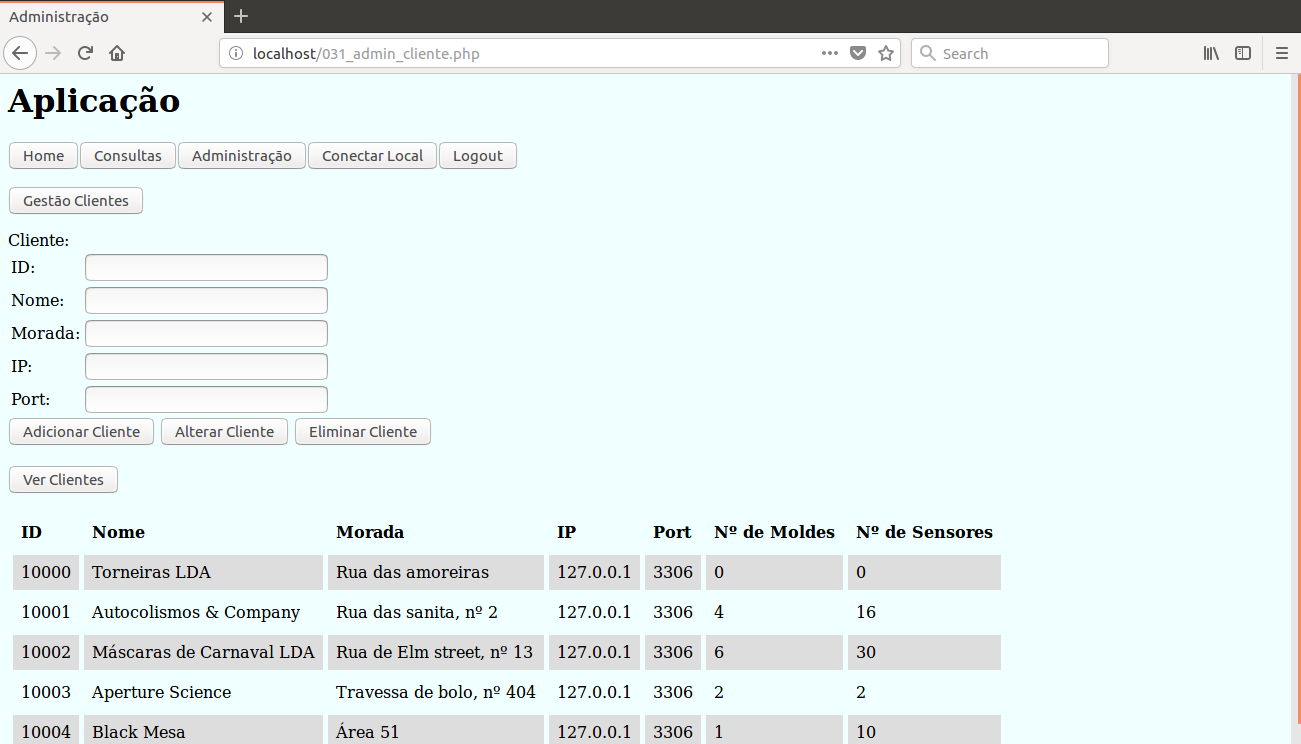
\includegraphics[width=0.9\textwidth]{administracao02} % Include the image placeholder.png
		\caption{Área de Gestão de Clientes sem conexão local}
		\label{fig:admin3}
	\end{center}
\end{figure}
\newpage
As áreas de Gestão de Moldes e Gestão de Sensores demonstradas nas Figuras \ref{fig:admin9} e \ref{fig:admin10}, permitem ao utilizador criar e apagar moldes e sensores, respetivamente. Estes dados são inseridos na base de dados temporária local, onde o utilizador pode criar e apagar moldes e sensores sem afetar o sistema. Desta forma confirma-se a informação introduzida antes de a inserir no sistema. Os botões de Criar e Apagar nestes formulários realizam \textit{queries} do tipo INSERT e DELETE, respetivamente.
	\begin{figure}[H]
		\centering
			\includegraphics[width=0.8\textwidth]{administracao05} % Include the image placeholder.png
			\caption{Área de Gestão de Moldes}
			\label{fig:admin9}
	\end{figure}
	\begin{figure}[H]
		\centering
			\includegraphics[width=0.8\textwidth]{administracao06} % Include the image placeholder.png
			\caption{Área de Gestão de Sensores}
			\label{fig:admin10}
	\end{figure}
Quando a informação dos moldes e sensores estiver completa, o botão Validar tenta registar os valores presentes na base de dados temporária local nas bases de dados central e local. Se a ação não executar com sucesso é retornado um erro \textit{MySQL} de forma a informar o utilizador. Se a ação executar com sucesso a base de dados temporária local é limpa e os valores são registados permanentemente nas bases de dados central e local, como representado nas Figuras \ref{fig:admin12} e \ref{fig:admin13}.\par
Depois de inseridos, moldes e sensores não podem ser eliminados via aplicação. Esta opção foi removida da aplicação para evitar erros, dado que apagar um molde em funcionamento faz com que se percam novos registos.
\begin{figure}[H]
	\centering
	\begin{minipage}{.5\textwidth}
		\begin{center}
			\includegraphics[width=0.9\textwidth]{administracao07} % Include the image placeholder.png
			\subcaption{Dados antes de serem validados}
			\label{fig:admin12}
		\end{center}
	\end{minipage}%
	\begin{minipage}{.5\textwidth}
		\begin{center}
			\includegraphics[width=0.9\textwidth]{administracao08} % Include the image placeholder.png
			\subcaption{Dados após serem validados}
			\label{fig:admin13}
		\end{center}
	\end{minipage}
	\caption{Função do botão Validar, onde os valores da base de dados temporária local são transferidos de forma permanente para as bases de dados central e local}
	\label{fig:admin11}
\end{figure}
Nas várias áreas de gestão existem os botões Ver Clientes, Ver Moldes e Ver Sensores que executam respetivamente as \textit{queries}:
\begin{lstlisting}[language = SQL]
1-	SELECT cl_ID, cl_nome, cl_morada, cl_IP, cl_port,
	COUNT(DISTINCT m_ID), COUNT(DISTINCT s_IDMolde, s_num)
	FROM clientes
	LEFT OUTER JOIN moldes ON cl_ID = m_IDCliente
	LEFT OUTER JOIN sensores ON m_ID = s_IDMolde
	GROUP BY cl_ID
	ORDER BY cl_ID
	
2-	SELECT m_IDCliente, m_ID, m_nome, m_descricao,
	COUNT(DISTINCT s_IDMolde, s_num)
	FROM clientes
	INNER JOIN moldes ON cl_ID = m_IDCliente
	LEFT OUTER JOIN sensores ON m_ID = s_IDMolde
	GROUP BY m_ID
	ORDER BY m_IDCliente, m_ID
	
3-	SELECT m_IDCliente, s_IDMolde, s_num, tipo_nome,
	s_nome, s_descricao
	FROM moldes
	INNER JOIN sensores ON m_ID = s_IDMolde
	INNER JOIN tipo ON s_tipo = tipo_id
	ORDER BY m_IDCliente, s_IDMolde, s_num
\end{lstlisting}
Estas \textit{queries} fornecem algumas informações contextuais para facilitar a navegação do utilizador.

\subsubsection{Conectar Local}
\label{subchap:local}
	\begin{figure}[H]
		\centering
			\includegraphics[width=0.9\textwidth]{local01} % Include the image placeholder.png
			\caption{Área Conectar Local onde se visualiza as bases de dados instaladas no sistema}
			\label{fig:local1}
	\end{figure}
A área de Conectar Local na \autoref{fig:local1} permite realizar uma conexão à base de dados local no servidor do cliente. Com recurso à \textit{query}:
\begin{lstlisting}[language = SQL]
	SHOW DATABASES
\end{lstlisting}
Obtém-se todas as bases de dados instaladas no servidor local. Do ponto de vista prático, cada cliente só terá uma base de dados local mas, para efeitos de desenvolvimento do projeto adotou-se esta vertente.
O botão Conectar inicia sessão na base de dados local escolhida e redireciona o utilizador para a página de Administração como se observar na \autoref{fig:local4}. O botão Desconectar termina esta sessão e redireciona o utilizador também para a página de Administração.
\newpage
\begin{figure}[H]
	\begin{center}
		\includegraphics[width=0.9\textwidth]{main03} % Include the image placeholder.png
		\caption{\textit{Main} com conexão local}
		\label{fig:local4}
	\end{center}
\end{figure}
	\begin{figure}[H]
		\centering
		\includegraphics[width=0.9\textwidth]{local02} % Include the image placeholder.png
		\caption{Área Criar Local cria a base de dados para o cliente selecionado no sistema em que se acede a aplicação}
		\label{fig:local2}
	\end{figure}
A área Criar Local na \autoref{fig:local2} permite instalar uma base de dados para um novo cliente. São considerados novos clientes todos os que não tenham moldes associados a si, esta informação obtém-se com a \textit{query}:
\newpage
\begin{lstlisting}[language = SQL]
	SELECT cl_ID, cl_nome, cl_morada, cl_IP, cl_port
	FROM
		(SELECT cl_ID, cl_nome, cl_morada, cl_IP, cl_port,
		COUNT(DISTINCT m_ID) AS n_moldes
		FROM clientes
		LEFT OUTER JOIN moldes ON cl_ID = m_IDCliente
		GROUP BY cl_ID) AS contagem
	WHERE n_moldes = 0
\end{lstlisting}
Escolhendo um cliente válido o botão Criar gera \textit{queries} para efetuar a instalação da base de dados local e definir as respetivas permissões. Estas \textit{queries} não são visíveis ao utilizador, assim sendo, o botão Copiar Query copia-as para a área de transferência e estas devem ser introduzidas no \textit{MySQL} com o comando colar, como representado na \autoref{fig:local5}.
\begin{figure}[H]
	\begin{center}
		\includegraphics[width=0.9\textwidth]{local03} % Include the image placeholder.png
		\caption{\textit{Queries} geradas para completar a instalação da base de dados no sistema local. Consistem nas permissões para os utilizadores que só podem ser garantidas via \textit{root} bem como informação para completar o sistema de dados}
		\label{fig:local5}
	\end{center}
\end{figure}
\newpage
Terminado a análise das funcionalidades da aplicação com a área de Instalar \textit{MySQL} na \autoref{fig:local3} que contém os passos para instalar o \textit{MySQL} num sistema \textit{Linux}.
\begin{figure}[H]
	\centering
	\includegraphics[width=0.9\textwidth]{local04} % Include the image placeholder.png
	\caption{Área Instalar \textit{MySQL} para instalar o \textit{software} com os comandos em \textit{Linux}}
	\label{fig:local3}
\end{figure}

\cleardoublepage
\chapter{Testes de Usabilidade}
\label{chap:usabilidade}

\cleardoublepage
\chapter{Conclusões}
\label{chap:conclusoes}
O desafio proposto consiste em monitorizar sensores remotamente. Para isto definiu-se como objetivos principais desenvolver uma rede de bases de dados e uma aplicação que permitisse interagir com elas. Estes objetivos foram concluídos com sucesso. Este capítulo contém comentários sobre o desempenho da solução desenvolvida e propostas para trabalhos futuros.

\section{Comentários}
\subsection{Infraestrutura de dados}
Em relação à infraestrutura proposta, esta cumpre todos os requisitos propostos de garantir uma transferência segura, confidencial e permanente de valores, criando um histórico dos moldes monitorizados. Consiste numa rede de bases de dados relacionais com uma central e uma local para cada cliente o que minimiza a perda de registos em caso de falha de conexão. Num programa de transferência de valores que coordena a transferência dos registos para o sistema central criando históricos das medições dos moldes. Noutro de gestão de \textit{backups} que limpa a base de dados central dos registos mais antigos e arquiva-os em ficheiros num repositório \textit{online}. Terminando com simuladores que substituem a aquisição de dados reais e permitem popular as bases de dados locais.\par 
Como definido nos objetivos esta solução não impõe restrições na instrumentação dos moldes. Para introduzir dados nas bases de dados locais pode ser utilizado qualquer sistema operativo e linguagem de programação desde que esta tenha protocolos de comunicação com \textit{MySQL} e gere \textit{queries} do tipo:
\begin{lstlisting}[language = SQL]
	INSERT INTO registos
	VALUES
	(molde, sensor, fase, data_hora, milissegundos, valor);
\end{lstlisting}
Na realidade esta infraestrutura pode ser utilizada em qualquer contexto de monitorização remota de sensores desde que seja desenvolvido um modelo de dados apropriado.\par

\subsubsection{Programa de transferência}
Este foi desenvolvido como sendo centralizado em vez de descentralizado, como demonstrado na \autoref{fig:conclusoes0}. Na versão centralizada, o sistema central tem de garantir a transferência de todos os clientes o que pode levar a um maior consumo de processador e consequente perda de desempenho. A versão descentralizada divide este consumo de processador pelos clientes dado que tem de ser os sistemas locais a garantir a transferência. Além disto, esta tem a vantagem do programa de transferência ser mais simples dado que não existe necessidade deste se dividir o programa. Assim sendo, na versão descentralizada, o programa assume o aspeto do subprograma da \autoref{fig:transferencia_subprograma} sem a necessidade de ser atualizado pelo utilizador.
\begin{figure}[H]
	\begin{center}
		\includegraphics[width=0.9\textwidth]{placeholder} % Include the image placeholder.png
		\caption{Exemplo da área Criar Local com criação das bases de dados e utilizadores via \textit{root} em vez de gerar \textit{queries} para o utilizador inserir manualmente no \textit{MySQL}}
		\label{fig:conclusoes0}
	\end{center}
\end{figure}
No entanto, esta versão tem desvantagens, se for necessário alterar o programa de transferência para adicionar novas funcionalidades tem de se aceder aos sistemas locais onde estes estão a ser executados. Esta ação de alterar o programa no cliente pode não ser trivial se, por exemplo, o sistema local do cliente estiver situado num país diferente. Outra vantagem da versão centralizada, esta permite limitar os acessos às bases de dados no sistema central. Como os programas comunicam entre si diretamente não se permite acesso remoto ao sistema central sem ser pela aplicação. Na versão descentralizada o sistema central tem de permitir uma conexão remota a partir do sistema local no cliente, isto pode constituir uma falha de segurança se não forem tomadas medidas para prevenir acessos indevidos ao sistema central.\par 
O programa cumpre os objetivos definidos, no entanto, o método para reiniciar o programa remotamente pela aplicação pode ser melhorado. Atualmente, o programa verifica com base num temporizador a base de dados regulação de procedimentos, dependendo deste temporizador pode existir alguma latência entre o ato de alterar o parâmetro \texttt{a\char`_transferencia} e o reiniciar propriamente dito do programa. Seria interessante desenvolver outro método que garanti-se que o programa de transferência reinicia-se sem latência.\par 
Além disto, durante o desenvolvimento do projeto, os simuladores nunca geraram registos com maior taxa do que o que o programa de transferência podia transferir. Se esta taxa for superada, a base local de onde provêm os registos ficará cada vez mais cheia o que pode levar a problemas de desempenho e, o programa, não está preparado para responder a situações destas. Sugere-se para futuros desenvolvimentos adaptar o programa de forma a que este possa aumentar automaticamente a sua taxa de transferência de registos. Duas soluções que podem ajudar a atingir este objetivo:
\begin{itemize}
	\item Aumentar a capacidade da \textit{string} que guarda os tuplos retornados
	\item Aumentar a quantidade de subprogramas para cada cliente
\end{itemize}

\subsubsection{Gestão de \textit{Backups}}
Este cumpre os objetivos definidos, no entanto, existem algumas limitações quanto ao método de realizar o \textit{backup}. Atualmente, o programa cria os ficheiros de \textit{backup} executando diretamente no terminal o comando \texttt{mysqldump} que permite definir a pasta de destino para o ficheiro criado:
\begin{lstlisting}[language = bash]
	mysqldump -u backupmanager -pbackup1234 backups_temp >
	~/Backups/backup.sql
\end{lstlisting}
Este comando também pode ser usado via \textit{query} para o \textit{MySQL}. No entanto, este não tem permissões para criar ficheiros fora da sua pasta principal, o que torna difícil mover os \textit{backups} para o repositório \textit{online}, dado que esta pasta principal está protegida com permissões de administrador. Na verdade é possível permitir o \textit{MySQL} criar ficheiros fora da sua pasta principal, só que isto pode constituir uma falha de segurança dado que é possível enviar comandos para o terminal via \textit{query}.\par 
Como referido anteriormente os ficheiros criados via \texttt{mysqldump} funcionam como ponto de restauro e requerem o uso de uma base de dados intermédia para proceder à sua concatenação. No entanto, foi a solução que permitiu a interação com um repositório \textit{online}.\par 
Uma solução explorada inicialmente para criar \textit{backups} consistia em ficheiros \texttt{.csv} que continham apenas registos com uma \textit{query} do estilo:
\begin{lstlisting}[language = SQL]
	SELECT *
	FROM backups.registos
	WHERE r_IDMolde = @IDMolde
	INTO OUTFILE
	'backup_@IDCliente_@IDMolde_@dataini_@datafim.csv'
	FIELDS TERMINATED BY ','
	ENCLOSED BY '"'
	LINES TERMINATED BY '\n'
\end{lstlisting}
Esta solução simplifica o processo de criação e concatenação dos \textit{backups} dado que esta não necessita de uma base de dados intermédia mas, tem algumas desvantagens. A desvantagem principal, como foi referido anteriormente, não se pode definir o diretório de criação do ficheiro fora da pasta principal do \textit{MySQL}. Além disto, para a informação puder ser carregada para a tabela registos só se pode fazer \textit{backup} desta tabela, o que pode levar à perda de informação relativa aos clientes, moldes e sensores se o planeamento dos ficheiros não for bem efetuado.\par 
Em futuros desenvolvimentos, se for definido que o diretório de criação dos \textit{backups} não é imperativo, deve-se dar ênfase a esta solução dado que este processo é mais simples e consequentemente mais rápido do que a solução usada neste projeto.

\subsection{Aplicação de gestão do sistema}
A aplicação cumpre os objetivos propostos de ser multiplataforma e garantir um acesso remoto à base de dados central, bem como gerir as informações dos clientes, moldes e sensores. Durante o desenvolvimento do projeto e testes de usabilidade verificou-se alguma falta de desempenho por parte da aplicação. Após alguns testes chegou-se à conclusão que esta falta de desempenho se devia ao \textit{hardware} utilizado e que um melhor computador e \textit{router} resolviam este problema.\par 
De momento o processo de instalação dos clientes ainda requer que o utilizador se ligue manualmente ao \textit{MySQL} para introduzir as \textit{queries} para criar os utilizadores e as bases de dados. Seria interessante em futuros desenvolvimentos chegar a uma solução que permitisse uma criação dos clientes diretamente pela aplicação como demonstrado na \autoref{fig:conclusoes1}.
\begin{figure}[H]
	\begin{center}
		\includegraphics[width=0.9\textwidth]{futuro01} % Include the image placeholder.png
		\caption{Exemplo da área Criar Local com criação das bases de dados e utilizadores via \textit{root} em vez de gerar \textit{queries} para o utilizador inserir manualmente no \textit{MySQL}}
		\label{fig:conclusoes1}
	\end{center}
\end{figure}
Além disto é necessário realizar uma revisão de segurança à aplicação. Um programador com intenções maliciosas pode aceder ao sistema pela aplicação e realizar comandos que podem comprometer o sistema.\par 
Apesar de serem necessários alguns ajustes de forma a melhorar o desempenho, a solução proposta da infraestrutura e aplicação é completamente funcional e pode ser já implementada numa fase experimental.

\section{Trabalhos Futuros}
Quanto à infraestrutura dos dados não foi definido como os sensores dos moldes serão ligados ao servidor local. No desenvolvimento deste projeto assumiu-se que todos os moldes estão ligados diretamente ao sistema local. No entanto, isto pode não ser sempre possível de se realizar por motivos físicos como demonstrado na \autoref{fig:conclusoes3}.
\begin{figure}[H]
	\begin{center}
		\includegraphics[width=0.9\textwidth]{placeholder} % Include the image placeholder.png
		\caption{Exemplo de problemas fisicos}
		\label{fig:conclusoes3}
	\end{center}
\end{figure}
Se se justificar, em vez de se ter um servidor local no cliente, ter um em cada molde molde. Esta adaptação irá criar uma maior quantidade de bases de dados locais mas isto não é problemático, se o modelo de dados e o programa de transferência forem adaptados para o efeito.\par
Quanto à aplicação, sugere-se que após uma apresentação inicial à empresa promotora, seja iniciado um processo iterativo de desenvolvimento para escolher e desenvolver novas funcionalidades que possam ser úteis e que não tenham sido abrangidas neste projeto, como por exemplo, a criação de utilizadores baseado no ID de trabalhador demonstrado na \autoref{fig:conclusoes2}, que pode depois servir para criar históricos das intervenções dos utilizadores nas bases de dados. Culminando numa estilização da aplicação para que esta tenha um aspeto mais amigável ao utilizador.
\begin{figure}[H]
	\begin{center}
		\includegraphics[width=0.9\textwidth]{futuro02} % Include the image placeholder.png
		\caption{Exemplo de área de Registar para criar utilizadores com base no ID de trabalhador e email}
		\label{fig:conclusoes2}
	\end{center}
\end{figure}
Sugere-se a criação de um sistema de notificações e monitorização automático dos moldes. Durante o desenvolvimento do projeto chegou-se à conclusão de que é impossível para um utilizador analisar manualmente milhões de registos de um molde e concluir se este está a funcionar corretamente, como demonstrado na \autoref{fig:conclusoes4}.
\begin{figure}[H]
	\begin{center}
		\includegraphics[width=0.9\textwidth]{placeholder} % Include the image placeholder.png
		\caption{Exemplo molde 4 dinamometros a sair da cena}
		\label{fig:conclusoes4}
	\end{center}
\end{figure}
Para auxiliar os utilizadores sugere-se criar um programa capaz de correr algoritmos que analisem constantemente o comportamento dos moldes. Este programa pode ser desenvolvido em \textit{softwares} mais sofisticados, como por exemplo \textit{MATLAB}, desde que estes tenham protocolos de comunicação com \textit{MySQL}. Mantendo em mente o ambiente \textit{Web}, sugere-se que este programa notifique os utilizadores via aplicação de gestão do sistema ou via email quando um molde começa a demostrar um comportamento errático.

%
% The bibliography
%
\cleardoublepage
\bibliographystyle{unsrt}
\bibliography{bib/own/molde.bib,bib/own/base_dados.bib,bib/own/software.bib}

%%\sloppy
%%\printbibliography[prenote=myprenote,title=References]
%\iffalse
%  % Use this is the final version
%  %  unsrt produces numbered entries, sorted by order of citation
%  %  plain produces numbered entries, sorted alphabetically
%  %  other styles are possible (I recommend the harvard package)
%  \bibliographystyle{unsrt}
%  %\bibliographystyle{plain}
%  \bibliography{molde}% replace by the name of name of your .bib file
%\else
%  % An example (the contents of the .bbl file)
%  \begin{thebibliography}{10}
%
%  \bibitem{Eliahou-1-1993-CLBNCL}
%  Shalom Eliahou.
%  \newblock The $3x+1$ problem: New lower bounds on nontrivial cycle lengths.
%  \newblock {\em Discrete Mathematics}, 118(1--3):45--56, 1993.
%
%  \bibitem{Garner-1981-1-OCA}
%  Lynn~E. Garner.
%  \newblock On the collatz $3n+1$ algorithm.
%  \newblock {\em Proceedings of the American Mathematical Society}, 82(1):19--22,
%    May 1981.
%  \end{thebibliography}
%\fi
\cleardoublepage

\end{document}
